
\chapter{Markov Chain}
Hasta este punto, el núcleo del análisis estocástico se ha sustentado sobre procesos \textbf{intercambiables}, donde el orden cronológico de las observaciones carece de impacto en la asignación de la probabilidad conjunta:
\begin{equation*}
    P(X_1 = x_1, \dots, X_m = x_m) = P(X_{\sigma_1} = x_{\sigma_1}, \dots, X_{\sigma_m} = x_{\sigma_m})
\end{equation*}
Las \textbf{redes bayesianas} (\textit{Bayesian Networks}), formalizadas intensamente por \textbf{Judea Pearl}, rompen este supuesto simétrico introduciendo una ordenación causal y asimétrica a través de estructuras de grafos.

\begin{definicion}
    Una \textbf{red bayesiana} parametriza las dependencias de un vector de variables aleatorias $\{X_1, X_2, \dots, X_n\}$ mediante un Grafo $G = (V, E)$, donde los vértices $V$ representan las variables ($1 \text{ v.a.} \in V$) y las aristas $E$ codifican las relaciones directas. Para garantizar la consistencia probabilística, el grafo debe ser un \textbf{DAG} (\textit{Directed Acyclic Graph}): dirigido (relaciones causa-efecto unívocas) y acíclico (ausencia de bucles cerrados).
\end{definicion}

\vspace{0.4cm}

\begin{center}
\begin{tabular}{ccc}
    \begin{minipage}{0.25\textwidth}
        \centering
        \textbf{Grafo No Válido (Con Ciclos)} \\
        \vspace{0.2cm}
        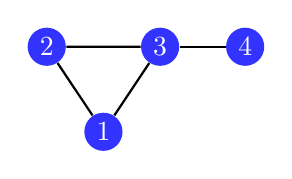
\begin{tikzpicture}[scale=0.9, every node/.style={circle, fill=blue!80, inner sep=2pt, text=white}]
            \node (1) at (0,0) {1};
            \node (2) at (-0.8,1.2) {2};
            \node (3) at (0.8,1.2) {3};
            \node (4) at (2,1.2) {4};
            \draw[thick] (1) -- (2) -- (3) -- (1);
            \draw[thick] (3) -- (4);
        \end{tikzpicture}
    \end{minipage} 
    & 
    \begin{minipage}{0.4\textwidth}
        \centering
        \textbf{Matriz de Adyacencia (Grafo No Dirigido)} \\
        \vspace{0.2cm}
        \[ 
        \begin{matrix}
            & 1 & 2 & 3 & 4 \\
            1 \\ 2 \\ 3 \\ 4
        \end{matrix} 
        \begin{pmatrix}
            0 & 1 & 1 & 0 \\
            1 & 0 & 1 & 0 \\
            1 & 1 & 0 & 1 \\
            0 & 0 & 1 & 0
        \end{pmatrix} 
        \]
    \end{minipage}
    &
    \begin{minipage}{0.3\textwidth}
        \centering
        \textbf{DAG Válido (Red Bayesiana)} \\
        \vspace{0.2cm}
        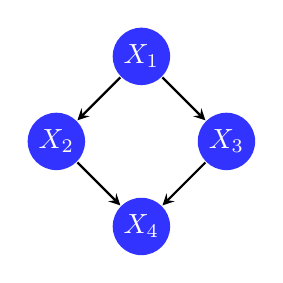
\begin{tikzpicture}[scale=0.9, every node/.style={circle, fill=blue!80, inner sep=2pt, text=white},->,>=stealth,thick]
            \node (x1) at (0,1.8) {$X_1$};
            \node (x2) at (-1.2,0.6) {$X_2$};
            \node (x3) at (1.2,0.6) {$X_3$};
            \node (x4) at (0,-0.6) {$X_4$};
            \draw (x1) -- (x2);
            \draw (x1) -- (x3);
            \draw (x2) -- (x4);
            \draw (x3) -- (x4);
        \end{tikzpicture}
    \end{minipage}
\end{tabular}
\end{center}

\noindent
Asumiendo por simplicidad que las variables aleatorias discretas toman valores sobre un soporte finito, nos interesa calcular su distribución finito-dimensional conjunta. De primeras para un sistema de cuatro variables aleatorias $\{X_1, X_2, X_3, X_4\}$, la probabilidad conjunta se puede factorizar mediante la regla de la cadena
\begin{align*}
    P(X_1 = x_1, X_2 = x_2, X_3 = x_3, X_4 = x_4) = & \; P(X_4 = x_4 \mid X_1 = x_1, X_2 = x_2, X_3 = x_3) \\
    & \cdot P(X_3 = x_3 \mid X_1 = x_1, X_2 = x_2) \\
    & \cdot P(X_2 = x_2 \mid X_1 = x_1) \\
    & \cdot P(X_1 = x_1)
\end{align*}

\begin{definicion}
    La \tbf{propieda de markov local} establece que para cada nodo $X_i$ de un DAG, la variable aleatoria $X_i$ es condicionalmente independiente de sus antepasados remotos dado el conjunto de sus padres directos, es decir, se obtiene toda su información relevante para predecir $X_i$ a partir de sus padres directos.
\end{definicion}

\noindent
Sabiendo que las flechas de un DAG codifican una \textbf{relación de causalidad directa}. Bajo la \textit{Propiedad de Márkov Local}, y sabiendo que los padres directos del nodo $X_4$ son exclusivamente $X_2$ y $X_3$, tenemos que
\begin{equation*}
    P(X_4 = x_4 \mid X_1 = x_1, X_2 = x_2, X_3 = x_3) = P(X_4 = x_4 \mid X_2 = x_2, X_3 = x_3)
\end{equation*}
Aplicando este filtro de independencia condicional a cada nodo, la probabilidad conjunta de la Red Bayesiana colapsa de forma exacta en el siguiente producto simplificado:
\begin{align*}
    P(X_1 = x_1, X_2 = x_2, X_3 = x_3, X_4 = x_4) = & \; P(X_4 = x_4 \mid X_2 = x_2, X_3 = x_3) \\
    & \cdot P(X_3 = x_3 \mid X_1 = x_1) \\
    & \cdot P(X_2 = x_2 \mid X_1 = x_1) \\
    & \cdot P(X_1 = x_1)
\end{align*}

\noindent
Las cadenas de márkov constituyen uno de los pilares más trascendentales de la teoría de procesos estocásticos y la estadística bayesiana moderna. Sus aplicaciones principales incluyen:
\begin{itemize}
    \item \textbf{MCMC (\textit{Markov Chain Monte Carlo}):} algoritmos de simulación computacional (como el muestreo de Gibbs o Metropolis-Hastings) orientados a extraer muestras de distribuciones posteriores complejas.
    \item \textbf{HMM (\textit{Hidden Markov Models}):} modelos donde los estados reales del sistema son latentes (ocultos) y solo se infieren a través de variables observables correlacionadas.
    \item \textbf{Modelización de Sistemas Físicos:} dinámica de fluidos, colas de espera masivas y transiciones en sistemas computacionales de estados finitos.
\end{itemize}
En esta sección trabajaremos con $(\Omega, \mathcal{F}, P)$ un espacio de probabilidad indexado por un parámetro de tiempo discreto $T = \{0, 1, 2, \dots\}$.

\begin{definicion}[Cadena de Márkov]
    Un proceso estocástico en tiempo discreto $\{X_m\}_{m \geq 0}$ definido sobre un \textbf{espacio de estados} $S$ discreto (finito o infinito numerable, tal que $S = \{1, \dots, g\}$, $S = \mathbb{N}$ o $S = \mathbb{Z}$) se denomina \textbf{cadena de márkov} si cumple con la \textbf{Propiedad de Márkov}:
    \begin{equation*}
        P(X_{m+1} = x_{m+1} \mid X_0 = x_0, X_1 = x_1, \dots, X_m = x_m) = P(X_{m+1} = x_{m+1} \mid X_m = x_m)
    \end{equation*}
    para todo $m \geq 0$ y para cualquier secuencia de estados $\{x_0, x_1, \dots, x_{m+1}\} \in S$ tales que \\ \mbox{$P(X_0 = x_0, \dots, X_m = x_m) > 0$}.
\end{definicion}

\observacion{
    La esencia de esta definición formal radica en el aislamiento de la memoria: el comportamiento futuro del proceso ($X_{m+1}$) condicionado a toda su historia evolutiva real depende única y exclusivamente del estado presente del sistema ($X_m$), volviéndose el pasado remoto completamente redundante.
}

\section{El Proceso de Simplificación Analítica}

\subsubsection{Descomposición de la Distribución Conjunta}
\noindent
Por la regla de la cadena de la probabilidad elemental, la distribución finito-dimensional conjunta de una trayectoria de longitud $m$ requiere almacenar toda la memoria histórica acumulada:
\begin{align*}
    P(X_1 = x_1, \dots, X_m = x_m) = & \; P(X_m = x_m \mid X_1 = x_1, \dots, X_{m-1} = x_{m-1}) \\
    & \cdot P(X_{m-1} = x_{m-1} \mid X_1 = x_1, \dots, X_{m-2} = x_{m-2}) \\
    & \;\; \vdots \\
    & \cdot P(X_2 = x_2 \mid X_1 = x_1) \cdot P(X_1 = x_1)
\end{align*}
Al invocar formalmente la Propiedad de Márkov, el condicionamiento masivo colapsa hacia el eslabón cronológico inmediato anterior, reduciendo la probabilidad conjunta al producto de transiciones locales:
\begin{equation*}
    P(X_1 = x_1, \dots, X_m = x_m) = P(X_1 = x_1) \prod_{i=2}^{m} P(X_i = x_i \mid X_{i-1} = x_{i-1})
\end{equation*}

\subsubsection{Homogeneidad Temporal}
\noindent
En una cadena de Márkov general, la regla de transición entre dos estados puede mutar según la edad del proceso, dependiendo intrínsecamente del paso del tiempo $m-1$:
\begin{equation*}
    P(X_m = y \mid X_{m-1} = x) = P_{m-1}(x, y)
\end{equation*}
Para estabilizar dinámicamente el modelo, se introduce el supuesto de \textbf{Homogeneidad en el Tiempo}. Se asume que las leyes que rigen los saltos son estacionarias e invariantes respecto al eje temporal:
\begin{equation*}
    P(X_m = y \mid X_{m-1} = x) = P(x, y) \quad \forall m \geq 1
\end{equation*}
Dadas estas dos condiciones, la convergencia de la propiedad de Márkov y la homogeneidad temporal, una Cadena de Márkov queda unívocamente determinada y gobernada por la interacción de solo dos elementos matemáticos:
\begin{enumerate}
    \item \textbf{Distribución Inicial ($p(x)$):} un vector de probabilidad que dicta el estado de arranque del sistema en el instante inicial:
    \begin{equation*}
        P(X_1 = x) = p(x) \quad \forall x \in S
    \end{equation*}
    \item \textbf{Probabilidad de Transición ($P(x,y)$):} la probabilidad estática de migrar desde un estado origen $x$ hacia un estado destino $y$ en un solo paso temporal discreto:
    \begin{equation*}
        P(X_{m+1} = y \mid X_m = x) = P(x, y) \quad \forall x,y \in S
    \end{equation*}
\end{enumerate}

\begin{ejemplo}
    Vamos a ver un ejemplo concreto de una cadena de Márkov con un espacio de estados finito $S = \{1, 2, 3\}$. Consideremos la probabilidad conjunta de que el proceso estocástico tome valores específicos en los tres primeros pasos de tiempo. Aplicando la regla de la cadena y la \underline{Propiedad de Markov} (falta de memoria), simplificamos la dependencia del pasado lejano:
    \begin{align*}
        P(X_1 = x, X_2 = y, X_3 = z) &= P(X_3 = z \mid X_2 = y, X_1 = x) \cdot P(X_2 = y \mid X_1 = x) \cdot P(X_1 = x) \\
        &= P(y, z) \cdot P(x, y) \cdot p(x)
    \end{align*}
    Para hallar la función de masa de probabilidad marginal en el tiempo $t=3$, aplicamos el teorema de la probabilidad total (marginalizando sobre todos los estados intermedios posibles $x, y \in S$):
    \[
    P(X_3 = z) = p_3(z) = \sum_{x, y \in S} P(y, z) P(x, y) \cdot p(x)
    \]
    Nos centramos ahora en un caso más simple con un espacio de estados binario $S = \{1, 2\}$, donde tenemos 
    \begin{itemize}
        \item  \textbf{Vector de Distribución Inicial ($\lambda_0$):} para un espacio de dos estados $S = \{1, 2\}$, definimos:
        \[ \lambda_0 = (p(1), p(2)) = \left( \frac{3}{4}, \frac{1}{4} \right) \]
        
        \item \textbf{Matriz de Transición ($P$):} es una matriz estocástica de dimensiones $g \times g$ (donde $g = |S|$) con entradas no negativas cuyas filas suman estrictamente 1.
        \[ P(x, y) = P(X_{m+1} = y \mid X_m = x) \qquad \sum_{y \in S} P(x, y) = 1 \]
        y viene dada de la siguiente forma
        \[ P = \begin{pmatrix} \frac{1}{4} & \frac{3}{4} \\[0.2cm] \frac{1}{2} & \frac{1}{2} \end{pmatrix} \]
        donde cada fila representa un estado origen y cada columna un estado destino, cumpliendo la condición de que la suma de cada fila sea igual a 1.
    \end{itemize}
    Calculemos de forma explícita la distribución en el paso $t=2$ analizando cada estado individualmente mediante la Ley de Probabilidad Total:
    \begin{align*}
    P(X_2 = 1) &= P(X_2 = 1 \mid X_1 = 1)P(X_1 = 1) + P(X_2 = 1 \mid X_1 = 2)P(X_1 = 2) \\
    &= \frac{1}{4} \cdot \frac{3}{4} + \frac{1}{2} \cdot \frac{1}{4} = \frac{3}{16} + \frac{1}{8} = \frac{5}{16} \\[0.3cm]
    P(X_2 = 2) &= P(X_2 = 2 \mid X_1 = 1)P(X_1 = 1) + P(X_2 = 2 \mid X_1 = 2)P(X_1 = 2) \\
    &= \frac{3}{4} \cdot \frac{3}{4} + \frac{1}{2} \cdot \frac{1}{4} = \frac{9}{16} + \frac{1}{8} = \frac{11}{16} \\
    &\text{Validación de la medida de probabilidad:} \quad \frac{5}{16} + \frac{11}{16} = 1
    \end{align*}

\vspace{0.4cm}

\noindent Este mecanismo algebraico tedioso se resuelve elegantemente en Data Science mediante el \textbf{álgebra lineal numérico} operando el vector fila por la matriz estocástica:

\vspace{0.3cm}
\noindent
\begin{minipage}{0.55\textwidth}
    \textbf{Paso 1 (Evolución a $\lambda_1$):}
    \[ \underbrace{\left( \frac{3}{4}, \frac{1}{4} \right)}_{\text{Estado Inicial $\lambda_0$}} \overbrace{\begin{pmatrix} \frac{1}{4} & \frac{3}{4} \\ \frac{1}{2} & \frac{1}{2} \end{pmatrix}}^{\text{{Matriz $P$}}} = \left( \frac{5}{16}, \frac{11}{16} \right) \]
    
    \textbf{Paso 2 (Evolución a $\lambda_2$):}
    \[ \left( \frac{5}{16}, \frac{11}{16} \right) \begin{pmatrix} \frac{1}{4} & \frac{3}{4} \\ \frac{1}{2} & \frac{1}{2} \end{pmatrix} = \left( \frac{3}{4}, \frac{1}{4} \right) \begin{pmatrix} \frac{1}{4} & \frac{3}{4} \\ \frac{1}{2} & \frac{1}{2} \end{pmatrix}^2 \]
\end{minipage}
\begin{minipage}{0.4\textwidth}
    \centering
    \textbf{Grafo de Transición} \\
    \vspace{0.2cm}
    \begin{tikzpicture}[
        ->, >=Stealth, 
        shorten >=1pt, 
        auto, 
        node distance=2cm, 
        state/.style={circle, draw=Blue, fill=Blue!5, minimum size=7mm, font=\small\bfseries}
    ]
        \node[state] (1) {1};
        \node[state] (2) [right=of 1] {2};

        \path (1) edge [loop left]  node {$\frac{1}{4}$} (1)
                  edge [bend left]  node {$\frac{3}{4}$} (2)
              (2) edge [bend left]  node {$\frac{1}{2}$} (1)
                  edge [loop right] node {$\frac{1}{2}$} (2);
    \end{tikzpicture}
\end{minipage}
\end{ejemplo}

\section{Time Homogeneous Markov Chains}

\begin{definicion}
    Un proceso estocástico en tiempo discreto $\{X_n\}_{n \ge 0}$ con espacio de estados finito o ajustable $S$ es una \textbf{cadena de markov homogénea en el tiempo} si sus probabilidades de transición condicionales satisfacen que, para todo paso temporal $m$, la probabilidad no depende del índice global sino únicamente de la distancia entre los estados:
    \begin{equation*}
        P(x, y) = P(X_{m+1} = y \mid X_m = x) = P(X_1 = y \mid X_0 = x) \quad \forall x, y \in S
    \end{equation*}
\end{definicion}



\noindent Las probabilidades de transición deben preservar la medida de probabilidad unitaria en su espacio mapeado:
\begin{equation*}
    \sum_{y \in S} P(x, y) = 1 \quad \forall x \in S
\end{equation*}

\begin{definicion}
    Una \textbf{matriz estocástica (o matriz de Markov)} es una matriz cuadrada cuyas entradas son no negativas y cumplen con la condición de que la suma de los elementos de cada una de sus filas es estrictamente igual a la unidad, es decir,
    $$\sum_{y \in S} P(x, y) = 1, \, \forall x \in S$$
\end{definicion}

\subsubsection{Distribución Finito-Dimensional del Proceso}
\noindent
En esta sección, veremos cómo calcular la probabilidad de que una Cadena de Markov describa una trayectoria exacta y específica a lo largo del tiempo. Para ello, definimos las funciones de masa de probabilidad en etapas tempranas o iniciales del sistema mediante vectores de estado:
\begin{itemize}
    \item \textbf{Distribución Inicial ($p_0$):} $p_0(x) = P(X_0 = x)$, la probabilidad del estado inicial en el tiempo $t=0$.
    \item \textbf{Distribución en el Paso Uno ($p_1$):} $p_1(x) = P(X_1 = x)$.
\end{itemize}

\noindent 
La distribución de probabilidad conjunta (distribución finito-dimensional) para una secuencia histórica de tamaño $n$ se descompone recursivamente mediante la propiedad de Markov como el producto encadenado de $n-1$ transiciones individuales y la masa inicial:
\begin{align*}
    P(X_1 = x_1, \dots, X_n = x_n) &= P(X_n = x_n \mid X_{n-1} = x_{n-1}) \cdots P(X_2 = x_2 \mid X_1 = x_1) \cdot P(X_1 = x_1) \nonumber \\
    &= \underbrace{P(x_{n-1}, x_n) \cdot P(x_{n-2}, x_{n-1}) \cdots P(x_1, x_2)}_{n-1 \text{ factores de transición}} \cdot p_1(x_1)
\end{align*}

\paragraph{Desplazamiento del Índice Temporal ($t=0$):}
Si reordenamos la indexación temporal para hacer explícito el origen cronológico desde el estado base $X_0 = x_0$, obtenemos la trayectoria exacta para un horizonte de $n$ pasos intermedios:
\begin{equation*}
    P(X_0 = x_0, X_1 = x_1, \dots, X_n = x_n) = \underbrace{P(x_{n-1}, x_n) \cdot P(x_{n-2}, x_{n-1}) \cdots P(x_0, x_1)}_{n \text{ factores de transición}} \cdot p_0(x_0)
\end{equation*}

\subsubsection{Distribución Marginal y Transición en $n$ Pasos}
\noindent
En esta sección, cambiaremos un poco la mentalidad, esta vez diremos ``No me importa el camino intermedio; solo quiero saber la probabilidad de estar en el estado $x_n$ en el paso $n$, habiendo empezado en algún lado", lo que significa que vamos a marginalizar sobre todos los estados intermedios posibles $x_0, x_1, \dots, x_{n-1} \in S$. \\

\noindent
Para recuperar la distribución marginal en cualquier etapa futura arbitraria $n$, denotada como $p_n(x_n) = P(X_n = x_n)$, aplicamos el Teorema de Probabilidad Total sumando sobre todas las historias o trayectorias internas posibles de los estados previos $x_0, x_1, \dots, x_{n-1} \in S$:
\begin{equation*}
    p_n(x_n) = \sum_{x_0 \in S} \sum_{x_1 \in S} \dots \sum_{x_{n-1} \in S} P(X_0 = x_0, X_1 = x_1, \dots, X_n = x_n)
\end{equation*}

\noindent Sustituyendo la ecuación estructural de la trayectoria conjunta de la sección anterior, el cálculo se reduce algebraicamente a:
\begin{align*}
    p_n(x_n) &= \sum_{x_0 \in S} \left[ \sum_{x_1, \dots, x_{n-1} \in S^{n-1}} P(x_{n-1}, x_n) \cdot P(x_{n-2}, x_{n-1}) \cdots P(x_0, x_1) \right] p_0(x_0) \nonumber \\
    &= \sum_{x_0 \in S} P^{(n)}(x_0, x_n) \, p_0(x_0)
\end{align*}
donde $P^{(n)}(x_0, x_n)$ representa la probabilidad de transición en $n$ pasos desde el estado inicial $x_0$ hasta el estado final $x_n$, obtenida al sumar sobre todos los caminos intermedios posibles. \\

\noindent
La sumatoria interna anidada representa algebraicamente la multiplicación iterada fila por columna de la matriz de transiciones $P$, dando lugar al elemento indexado de la matriz potencia $P^n$. Definimos matemáticamente dicho comportamiento como:
\begin{equation*}
    P^{(n)}(x_0, x_n) = P^n(x_0, x_n)
\end{equation*}
donde lo que se está haciendo es multiplicar la matriz de transición $P$ consigo misma $n$ veces, y luego tomar el elemento correspondiente a la fila $x_0$ y la columna $x_n$. Esto nos permite calcular la probabilidad de transición en $n$ pasos de manera eficiente utilizando álgebra lineal.

\observacion{
    Para ver la igualdad aplicada anteriormenten haremos este desarrollo paso a paso. Existe una equivalencia exacta entre el \textbf{Teorema de la Probabilidad Total} (sumar las rutas intermedias de una cadena) y la \textbf{multiplicación de matrices} (producto escalar de fila por columna). \\
 
    \noindent
    Sean dos matrices $A$ y $B$, su multiplicación para una celda específica se define mediante un índice compartido $k$:
    \begin{equation*}
        (A \times B)_{i,j} = \sum_{k} A(i,k) \cdot B(k,j)
    \end{equation*}
    Al calcular la probabilidad de transicionar de un estado inicial $x_0$ a un estado final $x_2$ en exactamente \textbf{2 pasos}, la teoría probabilística nos obliga a marginalizar sobre todos los estados intermedios posibles $x_1 \in S$:
    \begin{equation*}
        P^{(2)}(x_0, x_2) = \sum_{x_1 \in S} \underbrace{P(x_0, x_1)}_{\text{Fila } x_0 \text{ de } P} \cdot \underbrace{P(x_1, x_2)}_{\text{Columna } x_2 \text{ de } P}
    \end{equation*}
    Como el índice de la etapa intermedia $x_1$ ocupa la posición de columna en la primera matriz y de fila en la segunda, la estructura matemática es idéntica. Por lo tanto:
    \begin{itemize}
        \item Un sumatorio indexado ($\sum_{x_1}$) equivale a operar \textbf{un producto matricial} ($P \times P$).
        \item Una sumatoria anidada de $n-1$ variables temporales ($\sum_{x_1} \dots \sum_{x_{n-1}}$) equivale a la \textbf{multiplicación iterada} de la matriz por sí misma, resultando directamente en la matriz potencia $P^n$.
    \end{itemize}
}

\section{Master Equation}
\begin{definicion}
    Para una cadena de Markov homogénea en el tiempo, la probabilidad de transicionar desde un estado $x$ a un estado $y$ en exactamente dos pasos se calcula sumando sobre todos los estados intermedios posibles $z \in S$:
    \begin{equation*}
        P^{(2)}(x, y) = \sum_{z \in S} P(x, z) \cdot P(z, y)
    \end{equation*}
    lo que se llama \tbf{Chapman-Kolmogorov equation} para $n=2$. Para el caso general $n$, tenemos 
    \begin{equation*}
        P^{(n)}(x,y) = \sum_{i_1, \dots, i_{n-1} \in S} P(x, i_1) P(i_1, i_2) \dots P(i_{n-1}, y)
    \end{equation*}
\end{definicion}

\begin{teo}[Chapman-Kolmogorov Equation]
    Sea $\{X_n\}_{n \ge 0}$ una cadena de Markov homogénea en el tiempo. Para cualesquiera pasos temporales $n, m \ge 1$ y estados $x, y \in S$, la probabilidad de transicionar de $x$ a $y$ en $n+m$ pasos satisface
    $$P^{(n+m)}(x, y) = \sum_{z \in S} P^{(n)}(x, z) \cdot P^{(m)}(z, y)$$
\begin{proof}
    Para demostrarlo, debes apoyarnos firmemente en el Teorema de la Probabilidad Total condicionando en un ``tiempo intermedio'' exacto (el paso $n$).
    \begin{description}
        \item[\tbf{Paso 1.}] Plantear el objetivo analítico. Queremos calcular $P(X_{n+m} = y \mid X_0 = x)$.
        \item[\tbf{Paso 2.}] Introducir el estado intermedio. Para llegar a $y$ en el paso $n+m$, el sistema obligatoriamente tuvo que pasar por algún estado $z$ en el paso intermedio $n$. Aplicas el Teorema de la Probabilidad Total sumando sobre todo el espacio de estados $S$
        $$P(X_{n+m} = y \mid X_0 = x) = \sum_{z \in S} P(X_{n+m} = y, X_n = z \mid X_0 = x)$$
        \item[\tbf{Paso 3.}] Separar por la Regla de la Cadena, es decir, usando
        \begin{equation*}
            P(A\cap B) = P(A \mid B) \cdot P(B )
        \end{equation*}
        entonces abrimos la probabilidad conjunta del sumatorio
        $$\sum_{z \in S} P(X_{n+m} = y, X_n = z \mid X_0 = x)= \sum_{z \in S} P(X_{n+m} = y \mid X_n = z, X_0 = x) \cdot P(X_n = z \mid X_0 = x)$$
        \item[\tbf{Paso 4.}] Por la Propiedad de Markov, el futuro ($n+m$) solo depende del presente ($n$), por lo que el pasado ($X_0 = x$) se olvida en el primer factor
        $$P(X_{n+m} = y \mid X_n = z, X_0 = x) = P(X_{n+m} = y \mid X_n = z)$$
        Por Homogeneidad temporal, avanzar $m$ pasos desde el instante $n$ al $n+m$ es exactamente lo mismo que avanzar $m$ pasos desde el cero
        $$P(X_{n+m} = y \mid X_n = z) = P^{(m)}(z, y)$$
        \item[\tbf{Paso 5.}] Sustituyendo los términos simplificados, llegas directamente a la igualdad del teorema
        $$P^{(n+m)}(x, y) = \sum_{z \in S} P^{(m)}(z, y) \cdot P^{(n)}(x, z)$$
    \end{description}
\end{proof}
\end{teo}

\noindent
Nos interesa analizar la tasa de cambio de la probabilidad de estar en un estado específico $j$ entre el paso $m$ y el paso $m+1$. Evaluamos la diferencia:
\begin{equation*}
    P(X_{m+1} = j) - P(X_m = j)
\end{equation*}

\noindent Utilizando el Teorema de la Probabilidad Total y la propiedad de Markov, expandimos el primer término. Asimismo, multiplicamos el término $P(X_m = j)$ por $1$ en su forma estocástica unitaria, bajo la identidad indiscutible $\sum\limits_{x \in S} P(X_{m+1} = x \mid X_m = j) = 1$:
\begin{align*}
    P(X_{m+1} = j) &- P(X_m = j) = \\
    &= \sum_{x \in S} P(X_{m+1} = j \mid X_m = x)P(X_m = x) - \sum_{x \in S} P(X_{m+1} = x \mid X_m = j)P(X_m = j)= \\
    &= \sum_{x \in S} \Big[ \underbrace{P(X_{m+1} = j \mid X_m = x)P(X_m = x)}_{\text{Flujo de entrada hacia } j} - \underbrace{P(X_{m+1} = x \mid X_m = j)P(X_m = j)}_{\text{Flujo de salida desde } j} \Big]
\end{align*}

\noindent Reescribiendo en la notación simplificada de vectores de estado $p_m(j) = P(X_m = j)$ y elementos de la matriz de transición $P(x,j)$, obtenemos la forma discreta de la ecuación de balance:
\begin{equation*}
    p_{m+1}(j) - p_m(j) = \sum_{x \in S} \big[ P(x, j) p_m(x) - P(j, x) p_m(j) \big]
\end{equation*}
Para transicionar al tiempo continuo, parametrizamos los pasos temporales en función de intervalos pequeños $\Delta t$, de tal manera que el tiempo físico sea $t_m = m \Delta t$. Dividiendo toda la expresión por $\Delta t$, la ecuación se transforma en:
\begin{equation*}
    \frac{p_{t_m + \Delta t}(j) - p_{t_m}(j)}{\Delta t} = \sum_{x \in S} \big[ P(x, j) p_{t_m}(x) - P(j, x) p_{t_m}(j) \big] \cdot \frac{1}{\Delta t}
\end{equation*}

\noindent Al tomar el límite infinitesimal cuando $\Delta t \to 0$, las diferencias finitas se convierten en derivadas respecto al tiempo. Definimos ahora
\begin{equation*}
    \lim_{\Delta t \to 0} \frac{P(x, y)}{\Delta t} = Q(x, y) \quad (\text{para } x \neq y)
\end{equation*}
que son las \tbf{tasas de transición continuas} (elementos del generador infinitesimal o matriz $Q$) con la que el sistema decide abandonar tu estado $j$ para irse al estado $x$. \\

\noindent 
Llegamos formalmente a la \textbf{Ecuación Maestra en Tiempo Continuo}:
\begin{equation*}
    \frac{d p_t(j)}{dt} = \sum_{x \in S} \big[ Q(x, j) p_t(x) - Q(j, x) p_t(j) \big]
\end{equation*}
que representa la velocidad instantánea a la que cambia la probabilidad de estar en el estado $j$ en el momento exacto $t$, es decir, si es positiva el flujo neto de probabilidad hacia $j$ es mayor que el flujo de salida, y viceversa. 

\begin{definicion}
    Decimos que un vector de probabilidad $\pi = (\pi(x))_{x \in S}$ constituye una \textbf{distribución invariante} (o estacionaria) de la cadena si actúa como un punto fijo bajo el operador de transición, lo que significa que no sufre variaciones con el transcurso del tiempo:
    \begin{equation*}
        \pi P=\pi \quad \equiv \quad \pi(y) = \sum_{x \in S} \pi(x) P(x, y) \quad \forall y \in S
    \end{equation*}
    donde $P$ es la matriz de transición de la cadena de Markov en el caso discreto, y en el caso continuo sería $Q$.
\end{definicion}

\observacion{
    El vector de probabilidad $\pi$ representa el estado de equilibrio estadístico a largo plazo de la cadena de Markov. Una vez que el sistema adopta esta distribución de probabilidad, se congela dinámicamente: la probabilidad de estar en cada estado no volverá a cambiar jamás, sin importar cuántos pasos adicionales dé la cadena.
}



\subsection{Global Balance vs Detailed Balance}
\noindent
\begin{definicion}
    Para cualquier cadena de Markov, si existe una distribución invariante $\pi$, esta satisface de forma general la ecuación de \textbf{global balance}, lo que significa que el cambio neto de probabilidad en el equilibrio es nulo
    \begin{equation*}
        0 = \sum_{x \in S} \big[ P(x, j)\pi(x) - P(j, x)\pi(j) \big] \quad \forall j \in S
    \end{equation*}
    Una condición mucho más restrictiva (y sumamente útil en algoritmos de Data Science como MCMC) es el principio de \textbf{detailed balance}. Si existe un vector de probabilidad $\pi$ tal que el flujo de probabilidad entre cada par de estados se equilibra de forma aislada y simétrica:
    \begin{equation*}
        P(x, j)\pi(x) = P(j, x)\pi(j) \quad \forall x, j \in S
    \end{equation*}
\end{definicion}

\begin{definicion}
    Una cadena de Markov se dice \textbf{reversible} si existe una distribución invariante $\pi$ que satisface la condición de detailed balance, dada por la ecuación:
    \begin{equation*}
        P(x, j)\pi(x) = P(j, x)\pi(j) \quad \forall x, j \in S
    \end{equation*}
    donde para cada par de estados $x, j \in S$, el flujo de probabilidad desde $x$ hacia $j$ es exactamente igual al flujo de probabilidad desde $j$ hacia $x$ cuando el sistema está en equilibrio.
\end{definicion}

\paragraph{Consecuencia Inmediata (Matrices de Transición Simétricas):}
Si una cadena de Markov posee una probabilidad de transición \underline{estrictamente simétrica} entre sus estados intermedios ($P(j, x) = P(x, j)$ para todo $j \neq x$), se deduce directamente de la condición de reversibilidad que:
\begin{equation*}
    \frac{\pi(x)}{\pi(j)} = 1 \implies \pi(x) = \pi(j) \quad \forall x, j \in S
\end{equation*}
Esto demuestra matemáticamente que la distribución invariante de cualquier cadena con transiciones simétricas es una \textbf{distribución uniforme}, es decir, todos los estados tienen exactamente la misma probabilidad a largo plazo.

\begin{ejemplo}
    Consideremos una cadena de Markov de dos estados, $S = \{A, B\}$, caracterizada por la siguiente matriz estocástica de transición y su correspondiente grafo de estados:

    \noindent
    \begin{minipage}{0.45\textwidth}
        \centering
        \[ 
        P =
        \begin{pmatrix} 
        \frac{3}{4} & \frac{1}{4} \\[0.15cm] 
        \frac{1}{2} & \frac{1}{2} 
        \end{pmatrix} 
        \]
    \end{minipage}
    \begin{minipage}{0.5\textwidth}
        \centering
        \begin{tikzpicture}[
            ->, >=Stealth, 
            shorten >=1pt, 
            auto, 
            node distance=2.5cm, 
            state/.style={circle, draw=Blue, fill=Blue!5, minimum size=8mm, font=\small\bfseries}
        ]
            \node[state] (A) {A};
            \node[state] (B) [right=of A] {B};

            \path (A) edge [loop left]  node {$\frac{3}{4}$} (A)
                    edge [bend left]  node {$\frac{1}{4}$} (B)
                (B) edge [bend left]  node {$\frac{1}{2}$} (A)
                    edge [loop right] node {$\frac{1}{2}$} (B);
        \end{tikzpicture}
    \end{minipage}\\
    \noindent
    donde en la matriz de transición, la primera fila corresponde al estado $A$ y la segunda fila al estado $B$, mientras que las columnas representan los estados destino. Por ejemplo, $P(A, B) = \frac{1}{4}$ indica que la probabilidad de transicionar del estado $A$ al estado $B$ en un solo paso es del 25\%. \\

    \noindent 
    Buscamos un vector de probabilidad estacionario $\pi = (\pi_1, \pi_2)$ que actúe como punto fijo del sistema, es decir, que satisfaga la condición de invarianza $\pi P = \pi$:\
    \begin{equation*}
        (\pi_1, \pi_2) \begin{pmatrix} \frac{3}{4} & \frac{1}{4} \\[0.15cm] \frac{1}{2} & \frac{1}{2} \end{pmatrix} = (\pi_1, \pi_2)
    \end{equation*}

    \noindent Al realizar el producto matriz-vector, el problema algebraico se reduce a resolver el siguiente sistema de ecuaciones lineales simultáneas:
    \begin{equation*}
        \begin{cases} 
            \frac{3}{4}\pi_1 + \frac{1}{2}\pi_2 = \pi_1 \\[0.2cm] 
            \frac{1}{4}\pi_1 + \frac{1}{2}\pi_2 = \pi_2 
        \end{cases} 
        \implies \frac{1}{2}\pi_2 = \frac{1}{4}\pi_1 \implies \pi_1 = 2\pi_2
    \end{equation*}

    \noindent Imponiendo la condición necesaria de normalización para toda medida de probabilidad ($\pi_1 + \pi_2 = 1$):\
    \begin{equation*}
        2\pi_2 + \pi_2 = 1 \implies 3\pi_2 = 1 \implies \pi_2 = \frac{1}{3}, \quad \pi_1 = \frac{2}{3}
    \end{equation*}
\end{ejemplo}

\begin{ejemplo}[Descomposición Espectral (Eigen-extension)]
    Consideremos una cadena de Markov de dos estados cuya matriz de transición $P$ es \textbf{simétrica} y está parametrizada por las variables $a$ y $b$:
    \[ 
    P = \begin{pmatrix} a & b \\ b & a \end{pmatrix} \qquad \text{donde } 0 \le a, b \le 1 \quad \text{y} \quad a+b = 1
    \]
    Como las filas de toda matriz estocástica deben sumar estricta unidad, se cumple que $b = 1-a$. Dado que la matriz es simétrica ($P = P^T$), sus autovectores por la izquierda (distribuciones) coinciden espacialmente con sus autovectores por la derecha. El objetivo será ver el procedimiento a seguir para poder obtener 
    \begin{equation*}
        P^n
    \end{equation*}
    de forma sencilla.
    \begin{description}
        \item[\tbf{Calcular autovalores.}] Para hallar los autovalores de la matriz de transición, resolvemos el polinomio característico mediante el determinante $\det(P - \lambda I) = 0$:
        \[ 
        \det \begin{pmatrix} a-\lambda & b \\ b & a-\lambda \end{pmatrix} = 0 \implies (a-\lambda)^2 - b^2 = 0 
        \]
        Extrayendo la raíz cuadrada en ambos miembros obtenemos las dos soluciones del sistema:
        \begin{equation*}
            \begin{cases} 
                a-\lambda = -b \implies \lambda_1 = a+b = 1 \\ 
                a-\lambda = +b \implies \lambda_2 = a-b 
            \end{cases}
        \end{equation*}

        \begin{observacion}
            El primer autovalor siempre será $\lambda_1 = 1$ para cualquier matriz estocástica. El vector asociado a este autovalor determina la \textbf{distribución invariante} del sistema. Operando por la izquierda:
            \[ 
            (\pi_1, \pi_2) \begin{pmatrix} a & b \\ b & a \end{pmatrix} = 1 \cdot (\pi_1, \pi_2) \implies \pi_1 = \pi_2 = \frac{1}{2} \implies \pi = \left(\frac{1}{2}, \frac{1}{2}\right) 
            \]
        \end{observacion}
        \item[\tbf{Cálculo y Normalización Autovectores.}] Buscamos los autovectores columna por la derecha resolviendo el sistema homogéneo $(P - \lambda_i I)v = 0$:

        \begin{itemize}
            \item \textbf{Para $\lambda_1 = 1$:}
            \[ 
            \begin{pmatrix} a-1 & b \\ b & a-1 \end{pmatrix}\begin{pmatrix} x \\ y \end{pmatrix} = \begin{pmatrix} 0 \\ 0 \end{pmatrix} \xrightarrow{a-1 = -b} \begin{pmatrix} -b & b \\ b & -b \end{pmatrix}\begin{pmatrix} x \\ y \end{pmatrix} = \begin{pmatrix} 0 \\ 0 \end{pmatrix} \implies x = y \implies v_1 = \begin{pmatrix} 1 \\ 1 \end{pmatrix}
            \]
            Normalizando vectorialmente bajo la norma euclídea ($\|v\| = \sqrt{x^2+y^2}$), obtenemos
            $$v_1 = \begin{pmatrix} \frac{1}{\sqrt{2}} \\[0.1cm] \frac{1}{\sqrt{2}} \end{pmatrix}$$
            
            \item \textbf{Para $\lambda_2 = a-b$:}
            \[ 
            \begin{pmatrix} a-(a-b) & b \\ b & a-(a-b) \end{pmatrix}\begin{pmatrix} x \\ y \end{pmatrix} = \begin{pmatrix} 0 \\ 0 \end{pmatrix} \implies \begin{pmatrix} b & b \\ b & b \end{pmatrix}\begin{pmatrix} x \\ y \end{pmatrix} = \begin{pmatrix} 0 \\ 0 \end{pmatrix} \implies x = -y \implies v_2 = \begin{pmatrix} 1 \\ -1 \end{pmatrix}
            \]
            Normalizando euclídeamente obtenemos 
            $$v_2 = \begin{pmatrix} \frac{1}{\sqrt{2}} \\[0.1cm] -\frac{1}{\sqrt{2}} \end{pmatrix}$$
        \end{itemize}
        \item[\tbf{Diagonalización y Matriz de Transición Ortogonal.}] Al ser $P$ una matriz simétrica real, el teorema espectral garantiza que puede ser diagonalizada mediante una matriz ortogonal $U$ (donde la inversa coincide con su transpuesta, $U^{-1} = U^T$), construida acoplando los autovectores normalizados:
        \[ 
        U = \begin{pmatrix} \frac{1}{\sqrt{2}} & \frac{1}{\sqrt{2}} \\[0.15cm] \frac{1}{\sqrt{2}} & -\frac{1}{\sqrt{2}} \end{pmatrix} \implies U^T U = I
        \]
        Por lo tanto, la descomposición espectral de la matriz $P = U \Lambda U^T$ se escribe como:
        \[ 
        P = \begin{pmatrix} \frac{1}{\sqrt{2}} & \frac{1}{\sqrt{2}} \\[0.15cm] \frac{1}{\sqrt{2}} & -\frac{1}{\sqrt{2}} \end{pmatrix} \begin{pmatrix} 1 & 0 \\ 0 & a-b \end{pmatrix} \begin{pmatrix} \frac{1}{\sqrt{2}} & \frac{1}{\sqrt{2}} \\[0.15cm] \frac{1}{\sqrt{2}} & -\frac{1}{\sqrt{2}} \end{pmatrix} = \begin{pmatrix} \frac{1}{2} + \frac{a-b}{2} & \frac{1}{2} - \frac{a-b}{2} \\[0.15cm] \frac{1}{2} - \frac{a-b}{2} & \frac{1}{2} + \frac{a-b}{2} \end{pmatrix}
        \]

        \item[\tbf{Evolución Temporal.}]  La gran ventaja de la diagonalización es que calcular la evolución temporal a $n$ pasos se reduce a elevar el núcleo central de autavalores a la potencia $n$, dado que los términos ortogonales intermedios colapsan recursivamente ($U^T U = I$):
        \[ 
        P^n = (U \Lambda U^T)(U \Lambda U^T) \cdots (U \Lambda U^T) = U \Lambda^n U^T 
        \]
        \[ 
        P^n = \begin{pmatrix} \frac{1}{\sqrt{2}} & \frac{1}{\sqrt{2}} \\[0.15cm] \frac{1}{\sqrt{2}} & -\frac{1}{\sqrt{2}} \end{pmatrix} \begin{pmatrix} 1^n & 0 \\ 0 & (a-b)^n \end{pmatrix} \begin{pmatrix} \frac{1}{\sqrt{2}} & \frac{1}{\sqrt{2}} \\[0.15cm] \frac{1}{\sqrt{2}} & -\frac{1}{\sqrt{2}} \end{pmatrix} = \begin{pmatrix} \frac{1}{2} + \frac{(a-b)^n}{2} & \frac{1}{2} - \frac{(a-b)^n}{2} \\[0.2cm] \frac{1}{2} - \frac{(a-b)^n}{2} & \frac{1}{2} + \frac{(a-b)^n}{2} \end{pmatrix}
        \]
    \end{description}
    Ahora calculemos el límite para $n\to \infty$ y veámos que obtenemos. \\

    \noindent
    Como $0 \le a, b \le 1$ y $a+b=1$, la diferencia en valor absoluto satisface estrictamente $|a-b| < 1$ (salvo en casos triviales de matrices identidad o de permutación pura). Al calcular el límite cuando el tiempo tiende a infinito ($n \to \infty$), el segundo autovalor se desvanece por completo:
    \[ 
    \lim_{n \to \infty} (a-b)^n = 0 
    \]
    De este modo, la matriz de transiciones colapsa en el equilibrio estable y de largo plazo del sistema:
    \[ 
    \lim_{n \to \infty} P^n = \begin{pmatrix} \frac{1}{2} & \frac{1}{2} \\[0.15cm] \frac{1}{2} & \frac{1}{2} \end{pmatrix}
    \]
    donde 
    \begin{itemize}
        \item  La primera fila te dice qué pasa a largo plazo si empezaste en el estado 1: terminas con probabilidad $\left(\frac{1}{2}, \frac{1}{2}\right)$.  
        \item La segunda fila te dice qué pasa a largo plazo si empezaste en el estado 2: terminas con probabilidad $\left(\frac{1}{2}, \frac{1}{2}\right)$.  
    \end{itemize}
    Cada fila de la matriz resultante converge de manera idéntica hacia la distribución invariante uniforme $\pi = \left(\frac{1}{2}, \frac{1}{2}\right)$, demostrando que el sistema olvida por completo su estado inicial tras un horizonte temporal prolongado.    
\end{ejemplo}


\subsection{Teorema Espectral para Cadenas de Markov Reversibles}

\begin{teo}[Teorema Espectral para Cadenas de Markov Reversibles]
    Para cualquier cadena de Markov homogénea en el tiempo que sea \textbf{reversible}, la probabilidad de transición en $n$ pasos desde un estado $x$ a un estado $y$ puede descomponerse analíticamente en función de sus autovalores y autovectores mediante el teorema espectral
    \begin{equation}
        P^n(x,y) = \pi(y) + \sum_{i=2}^{g} \varphi_i(x)\varphi_i(y)\lambda_i^n
    \end{equation}
    donde:
    \begin{itemize}
        \item $\pi(y)$ representa la distribución invariante (asociada al primer autovalor $\lambda_1 = 1$).
        \item $\lambda_i$ son los autovalores secundarios, los cuales satisfacen rigurosamente $|\lambda_i| < 1$ (garantizando la convergencia).
        \item $\varphi_i$ son los autovectores ortonormalizados de la matriz de transición.
    \end{itemize}
\end{teo}

\begin{ejemplo}
    Validamos el teorema general utilizando la matriz simétrica de dos estados $S = \{1, 2\}$ analizada previamente:
    \[ 
    P = \begin{pmatrix} a & b \\ b & a \end{pmatrix} \qquad \text{con } a+b=1 
    \]
    Los elementos espectrales normalizados calculados para este sistema son:
    \begin{align*}
        \text{Distribución Invariante:} \quad &\pi = \left(\frac{1}{2}, \frac{1}{2}\right) \\[0.2cm]
        \text{Primer Autovalor:} \quad &\lambda_1 = 1 \;\,\longrightarrow \varphi_1 = \left(\frac{1}{\sqrt{2}}, \frac{1}{\sqrt{2}}\right) \\[0.15cm]
        \text{Segundo Autovalor:} \quad &\lambda_2 = a-b \longrightarrow \varphi_2 = \left(\frac{1}{\sqrt{2}}, -\frac{1}{\sqrt{2}}\right)
    \end{align*}
    La matriz de cambio de base ortogonal $U$ (construida acoplando los autovectores en columnas) cumple la condición de ortogonalidad unitaria ($U^T U = I$):
    \[
    U = \begin{pmatrix} \frac{1}{\sqrt{2}} & \frac{1}{\sqrt{2}} \\[0.15cm] \frac{1}{\sqrt{2}} & -\frac{1}{\sqrt{2}} \end{pmatrix}
    \]
    Veámos ahora si se cumple el teorema espectral al realizar la multiplicación de matrices $P^n = U \Lambda^n U^T$, la matriz de transición en $n$ pasos resulta:
    \[
    P^{(n)} = P^n = \begin{pmatrix} \frac{1}{2} + \frac{1}{2}(a-b)^n & \frac{1}{2} - \frac{1}{2}(a-b)^n \\[0.2cm] \frac{1}{2} - \frac{1}{2}(a-b)^n & \frac{1}{2} + \frac{1}{2}(a-b)^n \end{pmatrix}
    \]
    A continuación, descomponemos cada celda de la matriz para demostrar que coincide con la estructura del teorema general 
    $$P^n(x,y) = \pi(y) + \varphi_2(x)\varphi_2(y)\lambda_2^n$$
    véamoslo
    \begin{align*}
        P^n(1,1) &= \frac{1}{2} + \frac{1}{2}(a-b)^n = \pi(1) + \varphi_2^2(1) \lambda_2^n \\[0.2cm]
        P^n(1,2) &= \frac{1}{2} - \frac{1}{2}(a-b)^n = \pi(2) + \varphi_2(1)\varphi_2(2) \lambda_2^n \\[0.2cm]
        P^n(2,1) &= \frac{1}{2} - \frac{1}{2}(a-b)^n = \pi(1) + \varphi_2(2)\varphi_2(1) \lambda_2^n \\[0.2cm]
        P^n(2,2) &= \frac{1}{2} + \frac{1}{2}(a-b)^n = \pi(2) + \varphi_2^2(2) \lambda_2^n
    \end{align*}
\end{ejemplo}

\section{Ehrenfest Urn Model}
El Modelo de Urna de Ehrenfest fue publicado originalmente por Paul y Tatiana Ehrenfest en 1907 y 1911. Es una herramienta clásica para modelar la difusión de partículas y estudiar la mecánica estadística mediante cadenas de Markov. \\


\subsubsection{Configuración del Modelo de Microestados}
\noindent
Definiremos el modelo de urnas de Ehrenfest con un ejemplo simple usando $n=3$ bolas y $g=2$ contenedores. Imaginemos una urna dividida en dos compartimentos: izquierdo ($L$) y derecho ($R$), que albergan un total de $n=3$ bolas numeradas de forma única. En cada unidad discreta de tiempo, se selecciona una bola al azar con probabilidad uniforme ($1/n = 1/3$) y se traslada al compartimento opuesto.

\begin{center}
\begin{minipage}{0.4\textwidth}
    \centering
    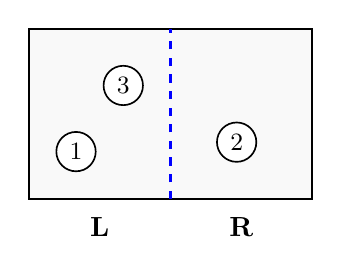
\begin{tikzpicture}[scale=1.2, semithick]
        % Contenedor de la urna
        \draw[thick, fill=gray!5] (0,0) rectangle (3, 1.8);
        \draw[thick, dashed, Blue] (1.5,0) -- (1.5, 1.8);
        \node[font=\bfseries] at (0.75, -0.3) {L};
        \node[font=\bfseries] at (2.25, -0.3) {R};
        
        % Ubicación de las partículas (ejemplo de microestado)
        \node[circle, draw=Black, fill=white, inner sep=1pt, minimum size=0.5cm, font=\small] (b1) at (0.5, 0.5) {1};
        \node[circle, draw=Black, fill=white, inner sep=1pt, minimum size=0.5cm, font=\small] (b3) at (1.0, 1.2) {3};
        \node[circle, draw=Black, fill=white, inner sep=1pt, minimum size=0.5cm, font=\small] (b2) at (2.2, 0.6) {2};
    \end{tikzpicture}
\end{minipage}
\begin{minipage}{0.5\textwidth}
    Asignamos un indicador binario $X_i$ para denotar la posición de la bola $i$:
    \begin{align*}
        \widetilde{X}_1 = L &\longleftrightarrow X_1 = 1 \quad (\text{Bola 1 en } L) \\
        \widetilde{X}_2 = R &\longleftrightarrow X_2 = 0 \quad (\text{Bola 2 en } R) \\
        \widetilde{X}_3 = L &\longleftrightarrow X_3 = 1 \quad (\text{Bola 3 en } L)
    \end{align*}
    El vector binario del sistema describe por completo el \textbf{microestado} exacto del proceso (e.g., el estado actual es $101$).
\end{minipage}
\end{center}

\subsubsection{Cadena de Markov de Microestados ($S_I$)}
\noindent
Si definimos el espacio de estados $S_I$ basándonos en la configuración individual de cada partícula, existen $2^n = 2^3 = 8$ estados posibles indexados en binario desde $000$ hasta $111$. Dado que en cada paso elegimos exactamente una bola entre las 3 disponibles con igual probabilidad, la matriz estocástica de transición es:

\[
P_I = 
\begin{matrix}
    & \begin{matrix} \text{\footnotesize 000} & \text{\footnotesize 001} & \text{\footnotesize 010} & \text{\footnotesize 100} & \text{\footnotesize 011} & \text{\footnotesize 101} & \text{\footnotesize 110} & \text{\footnotesize 111} \end{matrix} \\
    \begin{matrix} \text{\footnotesize 000} \\ \text{\footnotesize 001} \\ \text{\footnotesize 010} \\ \text{\footnotesize 100} \\ \text{\footnotesize 011} \\ \text{\footnotesize 101} \\ \text{\footnotesize 110} \\ \text{\footnotesize 111} \end{matrix} &
    \begin{bmatrix}
        0 & 1/3 & 1/3 & 1/3 & 0 & 0 & 0 & 0 \\
        1/3 & 0 & 0 & 0 & 1/3 & 1/3 & 0 & 0 \\
        1/3 & 0 & 0 & 0 & 1/3 & 0 & 1/3 & 0 \\
        1/3 & 0 & 0 & 0 & 0 & 1/3 & 1/3 & 0 \\
        0 & 1/3 & 1/3 & 0 & 0 & 0 & 0 & 1/3 \\
        0 & 1/3 & 0 & 1/3 & 0 & 0 & 0 & 1/3 \\
        0 & 0 & 1/3 & 1/3 & 0 & 0 & 0 & 1/3 \\
        0 & 0 & 0 & 0 & 1/3 & 1/3 & 1/3 & 0
    \end{bmatrix}
\end{matrix}
\]

\noindent La distribución invariante uniforme para este espacio de microestados es simétrica y de igual probabilidad:
\begin{equation}
    \pi_I = \Big( \underbrace{\frac{1}{8}}_{000}, \underbrace{\frac{1}{8}}_{001}, \underbrace{\frac{1}{8}}_{010}, \underbrace{\frac{1}{8}}_{100}, \underbrace{\frac{1}{8}}_{011}, \underbrace{\frac{1}{8}}_{101}, \underbrace{\frac{1}{8}}_{110}, \underbrace{\frac{1}{8}}_{111} \Big)
\end{equation}

\subsubsection{Cadena de Macroestados o de Conteo ($S_S$)}
\noindent
Para simplificar el sistema numéricamente, podemos definir una variable macroscópica de interés: el número total de bolas presentes en el compartimento izquierdo, denotado como 
$$Y_1 = \sum_{i=1}^{n} X_i$$
y el nuevo espacio reducido de estados es simplemente $S_S = \{0, 1, 2, 3\}$. Las leyes de transición para este conteo dependen directamente del número actual de bolas en $L$:
\begin{itemize}
    \item Si hay $k$ bolas en $L$, la probabilidad de elegir una de ellas y moverla a $R$ (pasando al estado $k-1$) es 
    $$\frac{k}{n}$$
    \item La probabilidad de elegir una de las $n-k$ bolas de $R$ y moverla a $L$ (pasando al estado $k+1$) es 
    $$\frac{n-k}{n}$$
\end{itemize}
La matriz de transición colapsada $P_S$ y su correspondiente distribución estacionaria $\pi_S$ son:
\[
P_S = 
\begin{matrix}
    & \begin{matrix} 0 & \;\;1 & \;\;2 & \;\;3 \end{matrix} \\
    \begin{matrix} 0 \\ 1 \\ 2 \\ 3 \end{matrix} &
    \begin{pmatrix}
        0 & 1 & 0 & 0 \\[0.1cm]
        1/3 & 0 & 2/3 & 0 \\[0.1cm]
        0 & 2/3 & 0 & 1/3 \\[0.1cm]
        0 & 0 & 1 & 0
    \end{pmatrix}
\end{matrix}
\qquad\qquad \pi_S = \left( \frac{1}{8}, \frac{3}{8}, \frac{3}{8}, \frac{1}{8} \right)
\]
Esta estructura matemática modela una \textbf{birth-death chain}, caracterizada como una caminata aleatoria con sesgo hacia el centro dentro de un retículo entero finito. Presenta las siguientes propiedades cruciales:
\begin{itemize}
    \item \textbf{Irreducible:} es posible acceder a cualquier estado desde cualquier otro en un número finito de pasos; el espacio de estados forma una única clase comunicante.
    \item \textbf{Periódica (Periodo $d=2$):} es imposible permanecer en el mismo estado en un solo paso ($P(x,x)=0, \, \forall x$). El sistema oscila de manera obligatoria entre estados pares e impares en cada transición temporal.
\end{itemize}

\begin{center}
    \begin{tikzpicture}[
        ->, >=Stealth, 
        shorten >=1pt, 
        auto, 
        node distance=2.5cm, 
        state/.style={circle, draw=Blue, fill=Blue!5, minimum size=10mm, font=\large\bfseries}
    ]
        \node[state] (0) {0};
        \node[state] (1) [right=of 0] {1};
        \node[state] (2) [right=of 1] {2};
        \node[state] (3) [right=of 2] {3};

        \path (0) edge [bend left=30]  node {$1$} (1)
              (1) edge [bend left=30]  node [swap] {$1/3$} (0)
                  edge [bend left=30]  node {$2/3$} (2)
              (2) edge [bend left=30]  node [swap] {$2/3$} (1)
                  edge [bend left=30]  node {$1/3$} (3)
              (3) edge [bend left=30]  node [swap] {$1$} (2);
    \end{tikzpicture}
\end{center}
En este caso tenemos un sistema que no converge por oscilación, ya que el periodo es $d=2$, lo cual es fácil de ver en la cadena de Markov de conteo. Por ejemplo, si comenzamos en el estado $0$, en el siguiente paso solo podemos ir al estado $1$, y desde allí solo podemos ir a los estados $0$ o $2$. Por lo tanto, no es posible permanecer en el mismo estado en un solo paso, lo que genera una oscilación entre estados pares e impares. 

\subsection{Birth-Death Chains}
\begin{definicion}
    Un proceso estocástico se define como una \tbf{birth-death chain} si, estando en un estado discreto $k \in \mathbb{N}$ (o en el retículo entero $\mathbb{Z}$), las únicas transiciones permitidas con probabilidad no nula en el siguiente paso de tiempo son hacia sus vecinos inmediatos o quedarse quieto:
    \[
    k \longrightarrow k-1 \quad (\text{Muerte}), \qquad k \longrightarrow k \quad (\text{Permanencia}), \qquad k \longrightarrow k+1 \quad (\text{Nacimiento})
    \]
    Cualquier otro movimiento de salto largo de largo alcance está estrictamente prohibido.
\end{definicion}

\begin{center}
    \begin{tikzpicture}[scale=1.2, semithick]
        \draw[thick, ->, >=Stealth] (0,0) -- (6,0);
        \foreach \x/\l in {1/{k-2}, 2/{k-1}, 3/{k}, 4/{k+1}, 5/{k+2}} {
            \draw (\x,0.1) -- (\x,-0.1) node[below, text=Green, font=\small\bfseries] {$\l$};
        }
        % Flechas de transición restringida
        \draw[->, Red, thick] (3,0.2) to[bend right=40] (2,0.2);
        \draw[->, Red, thick] (3,0.2) to[out=120,in=60,looseness=5] (3,0.2);
        \draw[->, Red, thick] (3,0.2) to[bend left=40] (4,0.2);
    \end{tikzpicture}
\end{center}
Seguiremos estudiando el modelo, para ello recordemos las probabilidades condicionales clásicas del modelo de conteo de Ehrenfest con $n$ partículas, donde las fronteras de la urna actúan como barreras reflejantes puras:
\begin{align*}
    P(Y_1(t+1) = k+1 \mid Y_1(t) = k) &= \frac{n-k}{n} & P(Y_1(t+1) = k-1 \mid Y_1(t) = k) &= \frac{k}{n} \\[0.2cm]
    P(Y_1(t+1) = k \mid Y_1(t) = k) &= 0 & P(Y_1(t+1) = 1 \mid Y_1(t) = 0) &= 1 \\[0.2cm]
    & & P(Y_1(t+1) = n-1 \mid Y_1(t) = n) &= 1
\end{align*}
donde tenemos $k$ partículas en la urna izquierda y $n-k$ partículas en la urna derecha.

\subsubsection{Versión Perezosa ($\alpha$-retrasada)}
\noindent
Para solucionar el problema que teníamos antes, es decir, que el sistema no converge por oscilación (periodo $d=2$), introduciremos una probabilidad de ``pereza'' $\alpha \in (0,1)$ para \underline{romper la periodicidad}. En cada unidad de tiempo, lanzamos una moneda sesgada: con probabilidad $\alpha$ el sistema decide quedarse congelado (no hacer nada), y con probabilidad $1-\alpha$ se elige una partícula al azar para cambiar de compartimento.

\begin{figure}[H]
    \centering
    \begin{tikzpicture}[scale=1.1, semithick]
        \draw[thick, fill=gray!5] (0,0) rectangle (2, 1.5);
        \draw[thick] (1,0) -- (1, 1.5);
        \node[font=\small\bfseries] at (0.5, -0.3) {L};
        \node[font=\small\bfseries] at (1.5, -0.3) {R};
        
        \node[circle, draw, inner sep=1pt, minimum size=0.4cm] at (0.5, 0.5) {\small 2};
        \node[circle, draw, inner sep=1pt, minimum size=0.4cm] at (1.5, 0.5) {\small 3};
        \node[circle, draw=Red, fill=Red!10, inner sep=1pt, minimum size=0.4cm] (1) at (1, 1.9) {\small 1};
        
        \draw[->, >=Stealth, thick] (1) to[bend right] node[left, font=\scriptsize] {$\alpha$ (Quedarse)} (0.4, 1.2);
        \draw[->, >=Stealth, thick] (1) to[bend left] node[right, font=\scriptsize] {$1-\alpha$ (Mover)} (1.6, 1.2);
    \end{tikzpicture}
    \vspace{0.2cm}
    
    \textbf{\tbf{Parámetro de Pereza:}} $\alpha \in (0,1)$
\end{figure}

\subsubsection{Matriz de Transición de Microestados Perezosa ($P_I$)}
\noindent
Al añadir la probabilidad $\alpha$ en la diagonal principal para representar el bucle de permanencia, la matriz de microestados distribuye el resto de la masa uniformemente entre las 3 partículas vecinas del hipercubo
\[
P_I = \begin{matrix}
    & \text{\footnotesize 000} & \text{\footnotesize 001} & \text{\footnotesize 010} & \text{\footnotesize 100} & \text{\footnotesize 011} & \text{\footnotesize 101} & \text{\footnotesize 110} & \text{\footnotesize 111} \\
    \text{\footnotesize 000} & \alpha & \frac{1-\alpha}{3} & \frac{1-\alpha}{3} & \frac{1-\alpha}{3} & 0 & 0 & 0 & 0 \\
    \text{\footnotesize 001} & \frac{1-\alpha}{3} & \alpha & 0 & 0 & \frac{1-\alpha}{3} & \frac{1-\alpha}{3} & 0 & 0 \\
    \text{\footnotesize 010} & \frac{1-\alpha}{3} & 0 & \alpha & 0 & \frac{1-\alpha}{3} & 0 & \frac{1-\alpha}{3} & 0 \\
    \text{\footnotesize 100} & \frac{1-\alpha}{3} & 0 & 0 & \alpha & 0 & \frac{1-\alpha}{3} & \frac{1-\alpha}{3} & 0 \\
    \text{\footnotesize 011} & 0 & \frac{1-\alpha}{3} & \frac{1-\alpha}{3} & 0 & \alpha & 0 & 0 & \frac{1-\alpha}{3} \\
    \text{\footnotesize 101} & 0 & \frac{1-\alpha}{3} & 0 & \frac{1-\alpha}{3} & 0 & \alpha & 0 & \frac{1-\alpha}{3} \\
    \text{\footnotesize 110} & 0 & 0 & \frac{1-\alpha}{3} & \frac{1-\alpha}{3} & 0 & 0 & \alpha & \frac{1-\alpha}{3} \\
    \text{\footnotesize 111} & 0 & 0 & 0 & 0 & \frac{1-\alpha}{3} & \frac{1-\alpha}{3} & \frac{1-\alpha}{3} & \alpha
\end{matrix}
\]
donde efectivamente cumple que las filas suman $1$ como debe ser
\begin{equation*}
    \alpha + 3\left(\frac{1-\alpha}{3}\right) = \alpha + 1 - \alpha = 1
\end{equation*}
La consecuencia principal de esta matriz es la \tbf{aperiodicidad}, pues al forzar que los elementos de la diagonal sean estrictamente positivos ($P(x,x) = \alpha > 0$), la cadena rompe los ciclos rígidos de alternancia par/impar. La cadena de Markov ahora es \textbf{irreducible y aperiódica}, lo que garantiza, según el Teorema Ergódico, el cumplimiento del límite de convergencia asintótica de largo plazo.


\subsubsection{Matriz de Transición de Macroestados Perezosa ($P_S$)}
\noindent
Colapsando el sistema al conteo masivo de partículas en el compartimento izquierdo, la matriz tridiagonal hereda el parámetro de retraso estructural:
\[
P_S = 
\begin{pmatrix}
    \alpha & 1-\alpha & 0 & 0 \\[0.15cm]
    \frac{1-\alpha}{3} & \alpha & \frac{2(1-\alpha)}{3} & 0 \\[0.15cm]
    0 & \frac{2(1-\alpha)}{3} & \alpha & \frac{1-\alpha}{3} \\[0.15cm]
    0 & 0 & 1-\alpha & \alpha
\end{pmatrix}
\]

\subsubsection{Simulación Asintótica }
\noindent
Si parametrizamos el modelo fijando un valor simétrico clásico de pereza $\alpha = \frac{1}{2}$, la matriz se simplifica aritméticamente. Al elevar la matriz estocástica a una potencia suficientemente grande ($n \gg 1$), el sistema converge de forma exacta hacia el equilibrio estacionario binomial independiente del estado inicial:

\[
\begin{pmatrix} 
    1/2 & 1/2 & 0 & 0 \\[0.1cm] 
    1/6 & 1/2 & 1/3 & 0 \\[0.1cm] 
    0 & 1/3 & 1/2 & 1/6 \\[0.1cm] 
    0 & 0 & 1/2 & 1/2 
\end{pmatrix}^n
\quad \xrightarrow{\quad n \to \infty \quad} \quad
\begin{pmatrix} 
    1/8 & 3/8 & 3/8 & 1/8 \\[0.1cm] 
    1/8 & 3/8 & 3/8 & 1/8 \\[0.1cm] 
    1/8 & 3/8 & 3/8 & 1/8 \\[0.1cm] 
    1/8 & 3/8 & 3/8 & 1/8 
\end{pmatrix}
\]

\noindent 
Cada fila de la matriz límite se ha convertido en una copia exacta del vector estacionario 
$$\pi_S = \left(\frac{1}{8}, \frac{3}{8}, \frac{3}{8}, \frac{1}{8}\right)$$
validando numéricamente que la cadena de Markov perezosa ha alcanzado el equilibrio ergódico.


\section{Clasificación Topológica de Cadenas de Markov}
La estructura analítica de un espacio de estados $S$ se clasifica según la probabilidad de retorno a largo plazo:
\begin{itemize}
    \item \textbf{Estado Transitorio:} existe una probabilidad estrictamente positiva de que, una vez abandonado el estado, el proceso jamás regrese a él.
    \item \textbf{Estado Recurrente:} el proceso regresa al estado con probabilidad igual a la unidad de forma casi segura.
    \item \textbf{Conjunto Absorbente / Cerrado:} un subconjunto de estados del cual la cadena es incapaz de escapar una vez que ha ingresado en él.
\end{itemize}
\begin{definicion}
    El \tbf{tiempo de parada} $T_A$ para un conjunto absorbente $A \subset S$ se define como el primer instante de tiempo en que la cadena alcanza dicho conjunto
    \[
    T_A = \inf\{t \ge 0 : X_t \in A\}
    \]
\end{definicion}

\begin{ejemplo} 
    Consideremos un espacio de tres estados $S = \{A, B, C\}$ definido por la siguiente matriz de transición $P$:       \\
    \noindent
    \begin{minipage}{0.45\textwidth}
        \centering
        \[ 
        P =
        \begin{pmatrix} 
        0 & 1 & 0 \\ 
        0 & 0 & 1 \\ 
        0 & 1 & 0 
        \end{pmatrix} 
        \]
    \end{minipage}
    \begin{minipage}{0.5\textwidth}
        \centering
        \begin{tikzpicture}[
            ->, >=Stealth, shorten >=1pt, auto, node distance=2cm,
            state/.style={circle, draw=Blue, fill=Blue!5, minimum size=8mm, font=\small\bfseries}
        ]
            \node[state] (A) {A};
            \node[state] (B) [right=of A] {B};
            \node[state] (C) [right=of B] {C};

            \path (A) edge node {$1$} (B)
                (B) edge [bend left=25] node {$1$} (C)
                (C) edge [bend left=25] node {$1$} (B);
        \end{tikzpicture}
    \end{minipage}
    \vspace{0.4cm}

    \noindent 
    Si el proceso inicia en el estado $A$, se genera la trayectoria determinista inalterable: $$\boldsymbol{A \longrightarrow B \longrightarrow C \longrightarrow B \longrightarrow C \dots}$$
    donde tenemos
    \begin{itemize}
        \item \textbf{Estado Transitorio:} $A$ es transitorio; una vez que salta a $B$, la probabilidad de regresar a $A$ es $0$.
        \item \textbf{Conjunto Absorbente:} el par $\{B, C\}$ constituye una clase cerrada o conjunto absorbente de estados. Individualmente, $B$ y $C$ son \textbf{estados recurrentes}.
    \end{itemize}
    En Data Science, suele interesar calcular el tiempo de parada 
    $$T_{\{B,C\}} = \inf\{t \ge 0 : X_t \in \{B,C\}\}$$ 
    necesario para alcanzar dicha clase. Para esta matriz, partiendo de $A$, el tiempo es determinista
    $$T_{\{B,C\}} = 1$$
\end{ejemplo}

\subsection{Cadenas de Markov Deterministas}
\noindent
Las siguientes matrices ilustran comportamientos donde el azar es nulo (probabilidades puras $1$ o $0$), generando trayectorias cíclicas o estáticas rígidas
\begin{itemize}
    \item \tbf{Identidad (Estacionaria):} la cadena permanece en el mismo estado indefinidamente. Ejemplo en Figura \ref{fig:identidad}.
    \item \tbf{Trampa Absorbente dual:} dos estados absorbentes independientes, cada uno atrapando la cadena en su propio ciclo. Ejemplo en la Figura \ref{fig:trampaabsorbente}.
    \item \tbf{Oscilación Cíclica:} la cadena alterna entre dos estados de manera indefinida. Ejemplo en la Figura \ref{fig:oscilacionciclica}.
    \item \tbf{Permutación Cíclica (3 Estados):} la cadena recorre un ciclo de tres estados de forma repetitiva. Ejemplo en la Figura \ref{fig:permutacionciclica}.
\end{itemize}

\begin{figure}
    \centering
    \textbf{Identidad (Estacionaria)}
    \[ \begin{pmatrix} 1/2 & 1/2 & 0 \\ 0 & 0 & 1 \\ 0 & 0 & 1 \end{pmatrix}^* \]
    \begin{tikzpicture}[->, >=Stealth, shorten >=1pt, auto, node distance=1.5cm,
        state/.style={circle, draw=Black, fill=Black!5, minimum size=7mm, font=\small\bfseries}]
        \node[state] (A) {A}; \node[state] (B) [right=of A] {B}; \node[state] (C) [right=of B] {C};
        \path (A) edge [loop above] node {$1/2$} (A) edge node {$1/2$} (B)
              (B) edge node {$1$} (C) (C) edge [loop above] node {$1$} (C);
    \end{tikzpicture}
    \caption{Cadena de Markov determinista con comportamiento absorbente y estacionario.}
    \label{fig:identidad}
\end{figure}

\begin{figure}
    \centering
    \textbf{Trampa Absorbente dual}
    \[ \begin{pmatrix} 1 & 0 \\ 0 & 1 \end{pmatrix} \]
    \begin{tikzpicture}[->, >=Stealth, shorten >=1pt, auto, node distance=1.5cm,
        state/.style={circle, draw=Black, fill=Black!5, minimum size=7mm, font=\small\bfseries}]
        \node[state] (A) {A}; \node[state] (B) [right=of A] {B};
        \path (A) edge [loop above] node {$1$} (A) (B) edge [loop above] node {$1$} (B);
    \end{tikzpicture}
    \caption{Cadena de Markov con dos estados absorbentes independientes.}
    \label{fig:trampaabsorbente}
\end{figure}

\begin{figure}
    \centering
    \textbf{Oscilación Cíclica}
    \[ \begin{pmatrix} 0 & 1 \\ 1 & 0 \end{pmatrix} \]
    \begin{tikzpicture}[->, >=Stealth, shorten >=1pt, auto, node distance=1.5cm,
        state/.style={circle, draw=Black, fill=Black!5, minimum size=7mm, font=\small\bfseries}]
        \node[state] (A) {A}; \node[state] (B) [right=of A] {B};
        \path (A) edge [bend left=25] node {$1$} (B) (B) edge [bend left=25] node {$1$} (A);
    \end{tikzpicture}
    \caption{Cadena de Markov con oscilación cíclica entre dos estados.}
    \label{fig:oscilacionciclica}
\end{figure}

\begin{figure}
    \centering
    \textbf{Permutación Cíclica (3 Estados)}
    \[ P = \begin{pmatrix} 0 & 1 & 0 \\ 0 & 0 & 1 \\ 1 & 0 & 0 \end{pmatrix} \]
    \begin{tikzpicture}[->, >=Stealth, shorten >=1pt, auto, node distance=1.5cm,
        state/.style={circle, draw=Black, fill=Black!5, minimum size=7mm, font=\small\bfseries}]
        \node[state] (A) {A}; \node[state] (B) [right=of A] {B}; \node[state] (C) [below=1.2cm of A] {C};
        \path (A) edge node {$1$} (B) (B) edge node {$1$} (C) (C) edge node {$1$} (A);
    \end{tikzpicture}
    \caption{Cadena de Markov con permutación cíclica entre tres estados.}
    \label{fig:permutacionciclica}
\end{figure}

\begin{definicion}
    El \tbf{fenómeno de metaestabilidad} se refiere a la situación en la que un sistema estocástico parece estar en un estado estable durante un período prolongado, pero eventualmente transiciona a otro estado estable debido a perturbaciones pequeñas o aleatorias. Viene dado por una cadena con dos trampas absorbentes aisladas cuya matriz es la Identidad ($I$), donde introducimos una perturbación infinitesimal $\varepsilon > 0$ (donde $\varepsilon \ll 1$, por ejemplo $\varepsilon = 10^{-20}$), los muros puros se rompen:
    \[
    \begin{pmatrix} 1 & 0 \\ 0 & 1 \end{pmatrix} \quad \xrightarrow{\quad \text{Perturbación} \quad} \quad \begin{pmatrix} 1-\varepsilon & \varepsilon \\ \varepsilon & 1-\varepsilon \end{pmatrix}
    \]
\end{definicion}

\begin{observacion}
    Este fenómeno recibe el nombre de metaestabilidad, pues el sistema parece estable y congelado localmente, pero macroscópicamente evoluciona de manera lenta hacia una distribución uniforme.
\end{observacion}
El comportamiento en este fenómeno se ve de dos formas

\begin{itemize}
    \item \tbf{Comportamiento a corto plazo:} Si el proceso inicia en $A$, se mantendrá atrapado en $A$ durante un tiempo extremadamente largo ($1-\varepsilon \approx 1$). Localmente parece una cadena absorbente estática.
    \item \tbf{Comportamiento asintótico (Long-run):} Al ser una matriz simétrica perturbada, los estados se comunican y la cadena se vuelve \textbf{irreducible}. A largo plazo ($n \to \infty$), el sistema alcanzará un equilibrio perfecto y balanceado:
    \[ 
    \pi_A = \pi_B = \frac{1}{2} 
    \]
\end{itemize}

\section{Class Structures}

\begin{definicion}[Accesibilidad o Conducción]
    Se dice que el estado $i$ \textbf{conduce al} estado $j$ (notado como $i \to j$) si existe una probabilidad estrictamente positiva de visitar el estado $j$ en algún momento, dado que el sistema comenzó en el estado $i$:
    \[
    P(\exists n \geq 0 : X_n = j \mid X_0 = i) > 0
    \]
\end{definicion}

\begin{definicion}[Comunicación]
Se dice que el estado $i$ \textbf{se comunica con} el estado $j$ (notado como $i \longleftrightarrow j$) si se cumplen simultáneamente que $i \to j$ y $j \to i$.
\end{definicion}

\begin{teo}
    Para dos estados distintos $i \neq j$, las siguientes afirmaciones son equivalentes:
    \begin{enumerate}
        \item $i \to j$.
        \item Existen estados intermedios $i_1, i_2, \dots, i_{n-1}$ tales que $P_{i i_1} P_{i_1 i_2} \dots P_{i_{n-1} j} > 0$.
        \item $P_{ij}^{(n)} > 0$ para algún $n \geq 1$.
    \end{enumerate}

\begin{proof}
    La equivalencia se sostiene mediante las siguientes relaciones fundamentales.
    \begin{description}
        \item[$1) \iff 3)$] Para cualquier paso fijo $n$, el evento $\{X_n = j\}$ es un subconjunto del evento general de ``visitar $j$ alguna vez''. Por subaditividad (cota de Boole), podemos acotar superior e inferiormente:
        \[ 
        P_{ij}^{(n)} \leq P(\exists m \geq 0 : X_m = j \mid X_0 = i) \leq \sum_{m=0}^{\infty} P_{ij}^{(m)} 
        \]
        Si la probabilidad central es $> 0$, la suma del extremo derecho debe tener al menos un término estrictamente positivo. Inversamente, si algún $P_{ij}^{(n)} > 0$, la probabilidad central es obligatoriamente mayor que cero.
        \item[$2)\iff 3)$] Por la expansión de las ecuaciones de Chapman-Kolmogorov, sabemos que:
        \[ 
        P_{ij}^{(n)} = \sum_{i_1, \dots, i_{n-1} \in S} P_{i i_1} P_{i_1 i_2} \dots P_{i_{n-1} j} 
        \]
        Dado que todas las probabilidades de transición son no negativas ($P_{kl} \geq 0$), este sumatorio es estrictamente positivo si y solo si existe al menos un término (un camino específico) en el sumatorio cuyo producto sea estrictamente mayor que cero.
    \end{description}
\end{proof}
\end{teo}

\begin{prop}
    La relación de comunicación ``$\longleftrightarrow$'' es una \textbf{relación de equivalencia} sobre el espacio de estados $S$, de cadenas de Márkov.

\begin{proof}
    Debemos verificar tres propiedades fundamentales:
    \begin{enumerate}
        \item \textbf{Reflexiva ($i \longleftrightarrow i$):} Por definición, en el paso $n=0$, 
        $$P_{ii}^{(0)} = P(X_0 = i \mid X_0 = i) = 1 > 0$$ 
        por lo que $i \to i$.
        \item \textbf{Simétrica ($i \longleftrightarrow j \implies j \longleftrightarrow i$):} Se deriva directamente de la conmutatividad de la conjunción lógica en la definición del operador ($\longleftrightarrow$), veámoslo
        \begin{equation*}
            i \longleftrightarrow j \iff (i \to j) \land (j \to i) \iff (j \to i) \land (i \to j) \iff j \longleftrightarrow i
        \end{equation*}
        \item \textbf{Transitiva ($i \longleftrightarrow j \land j \longleftrightarrow k \implies i \longleftrightarrow k$):} 
        Si $i \to j$ y $j \to k$, existen $n, m \geq 0$ tales que $P_{ij}^{(n)} > 0$ y $P_{jk}^{(m)} > 0$. Por Chapman-Kolmogorov:
        \[
        P_{ik}^{(n+m)} = \sum_{l \in S} P_{il}^{(n)}P_{lk}^{(m)} \geq P_{ij}^{(n)}P_{jk}^{(m)} > 0 \implies i \to k
        \]
        Siguiendo el mismo argumento de forma inversa para $k \to j \to i$, se obtiene $k \to i$. Por lo tanto, $i \longleftrightarrow k$.
    \end{enumerate}
\end{proof}
\end{prop}



\begin{observacion}
    Como toda relación de equivalencia, la \underline{comunicación} divide al conjunto $S$ en clases de equivalencia mutuamente disjuntas llamadas \textbf{clases de comunicación}. Si todos los estados pertenecen a una única clase, la cadena se denomina \textbf{irreducible}.
\end{observacion}


\begin{ejemplo}
    Considere una cadena de Markov homogénea con espacio de estados $S = \{1, 2, 3, 4, 5, 6\}$ y matriz de probabilidad de transición $P$ dada por la siguiente estructura matricial:
    \[
    P = 
    \begin{pmatrix}
        1/2 & 1/2 & 0 & 0 & 0 & 0 \\
        0 & 0 & 1 & 0 & 0 & 0 \\
        1/3 & 0 & 0 & 1/3 & 1/3 & 0 \\
        0 & 0 & 0 & 1/2 & 1/2 & 0 \\
        0 & 0 & 0 & 0 & 0 & 1 \\
        0 & 0 & 0 & 0 & 1 & 0
    \end{pmatrix}
    \]
    El comportamiento dinámico de las transiciones e interconexiones de la cadena se puede visualizar de forma equivalente mediante el siguiente grafo dirigido:

    \begin{center}
        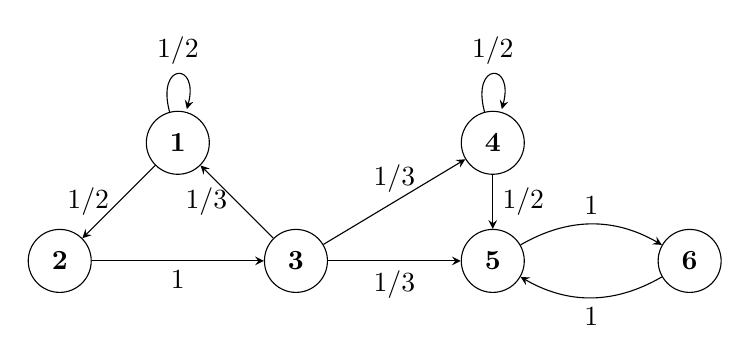
\begin{tikzpicture}[->, >=stealth, node distance=2cm, main/.style = {draw, circle, font=\bfseries, minimum size=0.8cm}]
            \node[main] (1) at (0,1.5) {1};
            \node[main] (2) at (-1.5,0) {2};
            \node[main] (3) at (1.5,0) {3};
            \node[main] (4) at (4,1.5) {4};
            \node[main] (5) at (4,0) {5};
            \node[main] (6) at (6.5,0) {6};
            
            \path (1) edge [loop above] node[above] {1/2} (1);
            \path (1) edge node[left] {1/2} (2);
            \path (2) edge node[below] {1} (3);
            \path (3) edge node[left] {1/3} (1);
            \path (3) edge node[above] {1/3} (4);
            \path (3) edge node[below] {1/3} (5);
            \path (4) edge [loop above] node[above] {1/2} (4);
            \path (4) edge node[right] {1/2} (5);
            \path (5) edge [bend left] node[above] {1} (6);
            \path (6) edge [bend left] node[below] {1} (5);
        \end{tikzpicture}
    \end{center}
    A partir de la relación de comunicación entre los estados del sistema, el espacio $S$ se descompone de forma única en las siguientes clases de equivalencia (particiones):
    \begin{itemize}
        \item $C_1 = \{1, 2, 3\} \longrightarrow$ Clase abierta y transitoria.
        \item $C_2 = \{4\} \longrightarrow$ Clase abierta y transitoria.
        \item $C_3 = \{5, 6\} \longrightarrow$ Clase \textbf{cerrada} y recurrente.
    \end{itemize}
\end{ejemplo}

\begin{definicion}[Clase Cerrada]
    Una clase de comunicación $C$ se dice que es \textbf{cerrada} si para todo estado $i \in C$, la condición $i \to j$ implica obligatoriamente que $j \in C$. Es decir, una vez que el proceso entra en una clase cerrada, no puede salir de ella.
\end{definicion}

\begin{definicion}[Estado Absorbente]
    Un estado $i \in S$ es \textbf{absorbente} si el subconjunto unipersonal $\{i\}$ forma por sí mismo una clase cerrada. Esto equivale a decir que $P_{ii} = 1$.
\end{definicion}

\begin{definicion}[Irreducibilidad]
    Una cadena de Markov se denomina \textbf{irreducible} si el espacio de estados total $S$ está constituido por una única clase de comunicación común. En otras palabras, todos los estados de la cadena se comunican mutuamente entre sí.
\end{definicion}

\subsection{Hitting Time \& Absorption Probabilities}
\noindent
Consideremos una cadena de Markov en tiempo discreto $(X_n)_{n \geq 0}$ con matriz de probabilidad de transición $P$ que opera sobre el espacio de estados $S$.

\begin{definicion}[Tiempo de Llegada / Hitting Time]
    El \textbf{tiempo de primera llegada} a un subconjunto de estados $A \subseteq S$ es una variable aleatoria $H^A: \Omega \to \{0, 1, 2, \dots\} \cup \{\infty\}$ que cuantifica el número mínimo de pasos necesarios para intersectar la región $A$:
    \[ 
    H^A(\omega) = \inf\{n \geq 0 : X_n(\omega) \in A\} 
    \]
    Bajo el convenio matemático estándar, si el conjunto es vacío, adoptamos que $\inf \emptyset = \infty$.
\end{definicion}

\begin{definicion}[Probabilidad de Llegada]
    La \tbf{probabilidad de llegada} o \textbf{hitting probability} es la probabilidad de alcanzar el conjunto de estados $A$ en tiempo finito partiendo inicialmente desde un estado específico $i$ se define como:
    \[ 
    h_i^A = P_i(H^A < \infty) = P(H^A < \infty \mid X_0 = i) 
    \]
\end{definicion}

\begin{observacion}
    Si la región de destino $A$ se corresponde con una clase cerrada de la cadena de Markov, la métrica $h_i^A$ adopta el nombre específico de \textbf{probabilidad de absorción}.
\end{observacion}

\begin{definicion}[Distribución Impropia]
    La variable aleatoria $H^A$ puede presentar una \tbf{distribución de probabilidad de carácter impropio} si existe una probabilidad residual no nula de no alcanzar nunca el conjunto objetivo $A$. En tal escenario, la suma sobre la trayectoria finita cumple:
    \[
    P_i(H^A < \infty) = \sum_{n=0}^{\infty} P_i(H^A = n) = \eta \leq 1
    \]
    De lo cual se deduce de forma inmediata la \tbf{probabilidad complementaria} para el horizonte infinito:
    \[
    P_i(H^A = \infty) = 1 - \eta
    \]
\end{definicion}

\begin{definicion}[Tiempo Medio de Llegada]
    El \textbf{tiempo esperado de llegada} al subconjunto $A$ partiendo desde el estado inicial $i$ viene dado por el valor esperado estadístico $E_i[H^A]$:
    \[ 
    k_i^A = E_i[H^A] = \sum_{n=0}^{\infty} n \, P_i(H^A = n) + \infty \cdot P_i(H^A = \infty) 
    \]
    donde si la probabilidad de no alcanzar el conjunto objetivo es nula ($P_i(H^A = \infty) = 0$), el término asintótico indeterminado desaparece de la ecuación de forma directa.
\end{definicion}

\subsubsection*{Interpretación Intuitiva de las Variables}
\begin{itemize}
    \item $h_i^A$: Cuantifica la probabilidad pura de lograr alcanzar el conjunto $A$ en algún punto de la historia futura.
    \item $k_i^A$: Modela el número esperado de pasos temporales que el sistema consumirá antes de tocar por primera vez la región $A$.
\end{itemize}

\begin{lema}
    Sea $T$ una variable aleatoria discreta bien definida que toma valores sobre el conjunto de los enteros no negativos ($\mathbb{N}_0$). Su esperanza matemática se puede calcular de manera alternativa a través de sus funciones de distribución acumulada complementaria mediante las identidades:
    \[
    E(T) = \sum_{n=0}^{\infty} nP(T = n) = \sum_{n=1}^{\infty} P(T \geq n)
    \]
\begin{proof}
    Expandiendo de forma explícita el operador del valor esperado lineal de la variable discreta por definición obtenemos:
    \[
    E(T) = \sum_{n=0}^{\infty} n \, P(T = n)
    \]
    Esta expresión se puede descomponer algebraicamente mediante una suma ordenada de probabilidades límite de cola superior como:
    \[
    E(T) = \sum_{n=1}^{\infty} P(T \geq n) = P(T \geq 1) + P(T \geq 2) + P(T \geq 3) + \dots
    \]
    Podemos validar analíticamente esta igualdad disponiendo los términos de las colas de probabilidad mediante un esquema de descomposición matricial infinita:
    \[
    \begin{array}{rcccccc}
        P(T \geq 1) & = & P(T=1) & + & P(T=2) & + & P(T=3) + \dots \\
        P(T \geq 2) & = &                  &   & P(T=2) & + & P(T=3) + \dots \\
        P(T \geq 3) & = &                  &   &                  &   & P(T=3) + \dots \\
    \end{array}
    \]
    Efectuando la agregación y suma por columnas verticales en el esquema anterior, se recupera exactamente la ponderación lineal original: un término para $P(T=1)$, dos términos para $P(T=2)$, tres términos para $P(T=3)$, y así sucesivamente, completando la demostración. \\


    \noindent
    Por analogía con el caso de variables continuas no negativas, este resultado equivale a evaluar la siguiente integral de supervivencia generalizada:
    \[
    E(T)= \int_{0}^{\infty}xf_T(x)\, dx=\int_{0}^{\infty} P(T > x) \, dx 
    \]
    ya que tenemos que

    $$P(T > x) = \int_{x}^{\infty} f_T(t) \, dt \implies \int_{0}^{\infty} P(T > x) \, dx = \int_{0}^{\infty} \left( \int_{x}^{\infty} f_T(t) \, dt \right) dx$$
    y por tanto
    $$\int_{0}^{\infty}P(T>x)\, dx=\int_{0}^{\infty} \left( \int_{0}^{t} dx \right) f_T(t) \, dt=\int_{0}^{\infty} t f_T(t) \, dt=E(T)$$
\end{proof}
\end{lema}


\begin{teo}
    El vector de probabilidades de primera llegada $h^A = (h_i^A)_{i \in S}$ es la solución no negativa mínima para el sistema de ecuaciones lineales:
    \[
    \begin{cases} 
        h_i^A = 1 & \text{para } i \in A \\ 
        h_i^A = \sum\limits_{j \in S} P_{ij} h_j^A & \text{para } i \notin A 
    \end{cases} \qquad (1)
    \]
    Minimalidad significa que si $x = (x_i)_{i \in S}$ es otra solución con $x_i \geq 0 \ \forall i$, entonces $x_i \geq h_i^A \ \forall i$.
\begin{proof}
    Analizaremos el comportamiento dinámico del sistema dividiéndolo según la naturaleza del estado inicial respecto al conjunto objetivo $A$:
    \begin{itemize}
        \item Si $X_0 = i$ con $i \in A$, entonces por definición el tiempo de llegada es inmediato, $H^A = 0$, por lo que 
        $$h_i^A = P_i(H^A < \infty) = 1$$
        \item Si $X_0 = i$ con $i \notin A$, entonces necesariamente el tiempo de primera llegada cumple que $H^A \geq 1$. Utilizando la propiedad de Markov espacial (pérdida de memoria) y la homogeneidad en el tiempo (la probabilidad pasar de $i$ a $j$ es la misma independientemente del instante $n$), evaluamos el condicionamiento al primer paso de la trayectoria:
        \[ 
        P(H^A < \infty \mid X_0 = i, X_1 = j) = P(H^A < \infty \mid X_1 = j) = h_j^A
        \]
        \noindent
        Aplicando el teorema de la probabilidad total mediante el condicionamiento exhaustivo sobre el primer estado visitado $X_1$, obtenemos:
        \begin{align*}
            h_i^A = P_i(H^A < \infty) &= \sum_{j \in S} P_i(H^A < \infty, X_1 = j) \\
            &\overset{(*)}{=} \sum_{j \in S} P(H^A < \infty \mid X_0 = i, X_1 = j) \, P(X_1 = j \mid X_0 = i) \\
            &= \sum_{j \in S} (P_{ij} \, h_j^A) = \sum_{j \in S} P_{ij} h_j^A
        \end{align*}
        donde en $(*)$ se ha aplicado $P(A \cap B) = P(A \mid B)P(B)$.
    \end{itemize}
    Esto demuestra que el vector real de probabilidades de llegada $h^A$ satisface formalmente el sistema lineal $(1)$. \\

    \noindent
    Demostraremos ahora la \underline{minimalidad}. Sea $x = (x_i)_{i \in S}$ un vector que representa cualquier solución no negativa arbitraria del sistema $(1)$. Evaluamos de igual forma por casos:
    \begin{itemize}
        \item Si $i \in A$, por diseño del sistema lineal se cumple de forma directa que $x_i = 1 = h_i^A$.
        \item Si $i \notin A$, la ecuación correspondiente nos permite descomponer el sumatorio sobre el espacio de estados separando la región objetivo $A$ de su complemento:
        \[
        x_i = \sum_{j \in S} P_{ij} x_j = \sum_{j \in A} P_{ij} x_j + \sum_{j \notin A} P_{ij} x_j
        \]
        Sustituyendo el valor fijo $x_j = 1$ para $j \in A$, y reconociendo que $\sum\limits_{j \in A} P_{ij} = P_i(X_1 \in A)$, el término se reescribe como:
        \[
        x_i = P_i(X_1 \in A) + \sum_{j \notin A} P_{ij} x_j
        \]
    \end{itemize}
    Procedemos a expandir la ecuación de forma iterativa sustituyendo la estructura analógica para el término no acotado $x_j$ dentro del sumatorio complementario:
    \[
    x_i = P_i(X_1 \in A) + \sum_{j \notin A} P_{ij} \left( P_j(X_1 \in A) + \sum_{k \notin A} P_{jk} x_k \right)
    \]
    Expandiendo los productos e identificando las probabilidades de transición conjuntas mediante la propiedad de Markov, obtenemos:
    \[
    x_i = P_i(X_1 \in A) + P_i(X_1 \notin A, X_2 \in A) + \sum_{j \notin A} \sum_{k \notin A} P_{ij} P_{jk} \, x_k
    \]
    donde para el término sumatorio del medio, hemos usado que 
    $$ P_j(X_1 \in A) = P(X_2 \in A \mid X_1 = j) $$
    gracias a aplicar la homogeneidad del tiempo, es decir, es lo mismo partir de $j$ (instante $0$) y tener en el instante $1$ un estado en $A$, a estar en el instante $1$ con estado $j$ y que el instante siguiente $2$ caiga en un estado de $A$. \\

    \noindent
    Al reiterar este procedimiento inductivo un número finito $m$ de pasos, la expresión adopta la siguiente forma generalizada:
    \begin{align*}
        x_i &= P_i(X_1 \in A) + P_i(X_1 \notin A, X_2 \in A) + \dots \\
        &\quad + P_i(X_1 \notin A, \dots, X_{m-1} \notin A, X_m \in A) + \sum_{j_1 \notin A} \dots \sum_{j_m \notin A} P_{i j_1} \dots P_{j_{m-1} j_m} x_{j_m}
    \end{align*}
    Reconociendo que la suma finita de probabilidades de trayectorias truncadas modela exactamente la probabilidad acumulada de alcanzar el conjunto $A$ en el paso $m$ o antes, simplificamos la expresión como:
    \[
    x_i = P_i(H^A \leq m) + \sum_{j_1 \notin A} \dots \sum_{j_m \notin A} P_{i j_1} P_{j_1 j_2} \dots P_{j_{m-1} j_m} x_{j_m}
    \]
    Dado que el vector de soluciones alternativo es estrictamente no negativo por hipótesis ($x \geq 0$) y las probabilidades de transición $P_{kl}$ son no negativas, el término del sumatorio múltiple residual es mayor o igual a cero. Por lo tanto, podemos establecer la siguiente desigualdad válida para cualquier entero $m$:
    \[
    x_i \geq P_i(H^A \leq m) \quad \forall m \geq 1
    \]
    Tomando el límite matemático cuando el horizonte de pasos tiende a infinito en ambos lados de la desigualdad, y aplicando la propiedad de continuidad de la medida de probabilidad para eventos monótonos crecientes, concluimos formalmente que:
    \[
    x_i \geq \lim_{m \to \infty} P_i(H^A \leq m) = P_i(H^A < \infty) = h_i^A
    \]
    Por lo tanto, queda demostrado que $x_i \geq h_i^A$ para todo estado $i \in S$, lo que confirma que el vector real $h^A$ constituye la solución mínima no negativa del sistema.
\end{proof}
\end{teo}

\begin{teo}
    El vector de tiempos esperados de primera llegada $k^A = (k_i^A)_{i \in S}$ es la solución no negativa mínima para el sistema de ecuaciones lineales:
    \[
    \begin{cases} 
        k_i^A = 0 & \text{para } i \in A \\ 
        k_i^A = 1 + \sum\limits_{j \notin A} P_{ij} k_j^A & \text{para } i \notin A 
    \end{cases} \qquad (2)
    \]
    Minimalidad significa que si $x = (x_i)_{i \in S}$ es otra solución con $x_i \geq 0 \ \forall i$, then $x_i \geq k_i^A \ \forall i$.

\begin{proof}
    Evaluamos el comportamiento del valor esperado analizando el origen del estado inicial de la cadena respecto al subconjunto $A$:
    \begin{itemize}
        \item Si $X_0 = i$ con $i \in A$, el tiempo de llegada se ejecuta instantáneamente de forma que $H^A = 0$. Por lo tanto, su valor esperado es nulo:
        \[
        k_i^A = E_i[H^A] = 0
        \]
        \item Si $X_0 = i$ con $i \notin A$, el proceso consume obligatoriamente un paso temporal elemental, implicando que $H^A \geq 1$. Aplicando la propiedad de Markov espacial y condicionando a la trayectoria del primer salto del sistema obtenemos la relación:
        \[
        E_i[H^A \mid X_1 = j] = 1 + E_j[H^A]
        \]
    \end{itemize}
    Desplegando el operador de la esperanza matemática mediante el teorema de la probabilidad total sobre el espacio exhaustivo del primer paso $X_1$, desarrollamos:
    \begin{align*}
        k_i^A = E_i(H^A) &= \sum_{j \in S} E_i(H^A \mid X_1 = j) \, P_i(X_1 = j) \\
        &= \sum_{j \in S} \big(1 + E_j(H^A)\big) \, P_i(X_1 = j) \\
        &= \sum_{j \in S} P_i(X_1 = j) + \sum_{j \in S} E_j(H^A) \, P_i(X_1 = j)
    \end{align*}
    Dado que $\sum_{j \in S} P_i(X_1 = j) = 1$, y reconociendo que para todo estado $j \in A$ se cumple la frontera $E_j(H^A) = k_j^A = 0$, el segundo sumatorio se restringe de forma natural a la región complementaria $j \notin A$:
    \[
    k_i^A = 1 + \sum_{j \notin A} k_j^A \cdot P_{ij} = 1 + \sum_{j \notin A} P_{ij} k_j^A
    \]
    Esto demuestra que el vector real $k^A$ satisface estructuralmente la relación lineal de recurrencia $(2)$.\\

    \noindent
    Demostraremos ahora la \underline{minimalidad}. Supongamos que existe un vector alternativo $y = (y_i)_{i \in S}$ que resuelve el sistema lineal $(2)$ con componentes no negativas. Evaluamos por regiones:
    \begin{itemize}
        \item Si $i \in A$, por la definición de la frontera superior del sistema se cumple directamente que $y_i = 0 = k_i^A$.
        \item Si $i \notin A$, la ecuación lineal que gobierna la dinámica se escribe como:
        \[
        y_i = 1 + \sum_{j \notin A} P_{ij} y_j
        \]
    \end{itemize}
    Procedemos a expandir la igualdad de manera iterativa sustituyendo la estructura analógica del término $y_j$ dentro del sumatorio complementario:
    \begin{align*}
        y_i &= 1 + \sum_{j \notin A} P_{ij} \left( 1 + \sum_{k \notin A} P_{jk} y_k \right) \\
        &= 1 + \sum_{j \notin A} P_{ij} + \sum_{j \notin A} \sum_{k \notin A} P_{ij} P_{jk} y_k
    \end{align*}
    Identificando los términos mediante medidas de trayectoria finita, observamos que $1 = P_i(H^A \geq 1)$ y que la probabilidad de transición complementaria mapea exactamente la cola superior $\sum_{j \notin A} P_{ij} = P_i(X_1 \notin A) = P_i(H^A \geq 2)$:
    \[
    y_i = P_i(H^A \geq 1) + P_i(H^A \geq 2) + \sum_{j \notin A} \sum_{k \notin A} P_{ij} P_{jk} y_k
    \]
    Reiterando este procedimiento de sustitución inductiva a lo largo de un horizonte finito de $m$ pasos, la expresión se generaliza como:
    \[
    y_i = P_i(H^A \geq 1) + \dots + P_i(H^A \geq m) + \sum_{j_1 \notin A} \dots \sum_{j_m \notin A} P_{i j_1} P_{j_1 j_2} \dots P_{j_{m-1} j_m} y_{j_m}
    \]
    Debido a la hipótesis de no negatividad del vector ($y \geq 0$) junto con la naturaleza no negativa de las celdas de la matriz de transición $P_{kl}$, el término de la sumatoria múltiple residual es acotado inferiormente por cero. Esto nos permite fijar la desigualdad para cualquier entero finito $m$:
    \[
    y_i \geq \sum_{l=1}^{m} P_i(H^A \geq l) \quad \forall m \geq 1
    \]
    Aplicando el límite matemático cuando el horizonte de pasos tiende a infinito en ambos extremos de la desigualdad, y recurriendo a la identidad de la esperanza por colas acumuladas de supervivencia para variables enteras no negativas ($\sum_{l=1}^{\infty} P(T \geq l) = E(T)$), concluimos:
    \[
    y_i \geq \lim_{m \to \infty} \sum_{l=1}^{m} P_i(H^A \geq l) = \sum_{l=1}^{\infty} P_i(H^A \geq l) = E_i(H^A) = k_i^A
    \]
    Por lo tanto, se verifica formalmente que $y_i \geq k_i^A$ para todo estado $i \in S$, demostrando que el vector de tiempos medios $k^A$ constituye la solución no negativa mínima del sistema lineal.
\end{proof}
\end{teo}

\subsection{Stopping Times \& Strong Markov Property}

\begin{definicion}[Tiempo de Parada / Stopping Time]
    Una variable aleatoria 
    $$T: \Omega \rightarrow \{0, 1, 2, \dots\} \cup \{\infty\}$$ 
    se denomina \textbf{tiempo de parada} si para cada instante finito $n \in \{0, 1, 2, \dots\}$, la ocurrencia o no del suceso $\{T = n\}$ está determinada única y exclusivamente por la trayectoria histórica acumulada del proceso hasta ese momento, es decir, depende únicamente de los valores de las variables aleatorias $X_0, X_1, \dots, X_n$.
\end{definicion}

\begin{ejemplo}
    A continuación, se analizan tres escenarios clásicos fundamentales para comprender la naturaleza de los tiempos de parada:

    \begin{enumerate}
        \item \textbf{El tiempo de primer paso a un estado $j$:} 
        Definido matemáticamente como el primer instante de tiempo estrictamente positivo en el cual la cadena visita el estado objetivo $j$:
        \[ 
        \tau_j = \inf\{n \geq 1 : X_n = j\} 
        \]
        Constituye un tiempo de parada bien definido puesto que el suceso se puede descomponer analíticamente a través de la historia observada hasta el paso $n$ como:
        \[ 
        \{ \tau_j = n \} = \{ X_0 \neq j, X_1 \neq j, \dots, X_{n-1} \neq j, X_n = j \} 
        \]
        Como esta condición solo inspecciona variables hasta el instante $n$, no requiere información del futuro.

        \item \textbf{El tiempo de primera llegada $H^A$ a un conjunto $A$:}
        Es un tiempo de parada dado que el suceso que describe que la primera colisión con la región $A$ ocurra exactamente en el paso $n$ se expresa de forma análoga mediante:
        \[ 
        \{ H^A = n \} = \{ X_0 \notin A, X_1 \notin A, \dots, X_{n-1} \notin A, X_n \in A \} 
        \]
        Este evento es medible respecto a la información disponible en el instante $n$.

        \item \textbf{El tiempo de última salida $L^A$ a un conjunto $A$ (No es tiempo de parada):}
        Definido como el instante temporal supremo en el cual el sistema interactúa por última vez con la región $A$:
        \[ 
        L^A = \sup\{n \geq 0 : X_n \in A\} 
        \]
        \textbf{Nota importante:} El tiempo de última salida \underline{no} constituye un tiempo de parada. Para poder afirmar con total certeza en el instante $n$ que el proceso ha visitado el conjunto $A$ por última vez, estaríamos obligados a conocer de antemano toda la trayectoria infinita futura del sistema ($X_{n+1}, X_{n+2}, \dots$) para certificar que el proceso jamás regresará a $A$. Al depender intrínsecamente de información del futuro, viola la definición fundamental.
    \end{enumerate}
\end{ejemplo}


\begin{teo}[Strong Markov Property]
    Sea $(X_n)_{n \geq 0}$ una cadena de Markov homogénea con vector de probabilidad inicial $\lambda$ y matriz de probabilidad de transición $P$. Sea $T$ un tiempo de parada respecto a la filtración natural del proceso $(X_n)_{n \geq 0}$. \\

    \noindent
    Entonces, condicionado al suceso $\{T < \infty\}$ y $\{X_T = i\}$, el proceso reiniciado $(X_{T+n})_{n \geq 0}$ es una cadena de Markov autónoma con vector de probabilidad inicial $\delta_i = (0, \dots, 0, 1, 0, \dots, 0)$ y matriz de probabilidad de transición $P$. Además, el proceso futuro $(X_{T+n})_{n \geq 0}$ es estadísticamente independiente de la trayectoria histórica pasada $X_0, X_1, \dots, X_T$.
\begin{proof}
    No es relevante y es muy complicada.
    % //TODO: entender demostración
%     Para facilitar el desarrollo algebraico, definimos el proceso desplazado en el tiempo como $Y_n = X_{T+n}$ para todo $n \geq 0$. La demostración se divide en dos fases analíticas fundamentales:

%     \subsection*{Fase 1: Verificación de la dinámica de Markov y homogeneidad}
%     Evaluamos la probabilidad de transición condicional de la estructura del nuevo proceso $Y_n$:
%     \begin{align*}
%         P(Y_m = i_m \mid Y_0 = i_0, \dots, Y_{m-1} = i_{m-1}) &= P(X_{T+m} = i_m \mid X_T = i_0, \dots, X_{T+m-1} = i_{m-1}) \\
%         &\overset{\text{(1)}}{=} P(X_m = i_m \mid X_0 = i_0, \dots, X_{m-1} = i_{m-1}) \\
%         &\overset{\text{(2)}}{=} P(X_m = i_m \mid X_{m-1} = i_{m-1}) \\
%         &\overset{\text{(3)}}{=} P(X_{m+T} = i_m \mid X_{m-1+T} = i_{m-1}) \\
%         &= P(Y_m = i_m \mid Y_{m-1} = i_{m-1})
%     \end{align*}
%     Las justificaciones de las igualdades críticas del colapso condicional son:
%     \begin{itemize}
%         \item[\textbf{(1)}] Aplicación de la \textbf{homogeneidad en el tiempo}: Desplazar el origen del cronómetro un número aleatorio de pasos $T$ preserva las mismas leyes distributivas que si iniciáramos en el origen absoluto $0$.
%         \item[\textbf{(2)}] Aplicación de la \textbf{propiedad de Markov estándar}: El comportamiento del sistema en el paso $m$ depende únicamente del estado inmediatamente precedente en el paso $m-1$, perdiendo la memoria de la historia previa.
%         \item[\textbf{(3)}] Aplicación inversa de la \textbf{homogeneidad temporal}: Permite volver a indexar el eje temporal añadiendo el factor del tiempo de parada $T$.
%     \end{itemize}

%     \subsection*{Fase 2: Demostración de la independencia del pasado}
%     Sea $H$ un suceso o evento arbitrario computable a partir de la trayectoria histórica del pasado del proceso, determinado únicamente por los estados $\{X_0, X_1, \dots, X_{T-1}\}$. 

%     Para evaluar la distribución conjunta condicionada a una absorción en tiempo finito, descomponemos el espacio muestral a través del teorema de la probabilidad total indexando sobre todos los valores posibles que puede adoptar el tiempo de parada $T = m$:
%     \begin{align*}
%         P(Y_1 = i_1, Y_2 = i_2, \dots, H \mid T < \infty, X_T = i_0) &= \sum_{m=0}^{\infty} P(Y_1 = i_1, Y_2 = i_2, \dots, H, T = m \mid T < \infty, X_T = i_0) \\
%         &= \sum_{m=0}^{\infty} P\big(Y_1 = i_1, Y_2 = i_2, \dots, H \cap \{T = m\} \mid T < \infty, X_T = i_0\big)
%     \end{align*}

%     Dado que por hipótesis $T$ constituye un \textbf{tiempo de parada}, el evento histórico acotado $H \cap \{T = m\}$ queda determinado unívocamente por las variables aleatorias del pasado $\{X_0, X_1, \dots, X_{m-1}\}$. Sustituyendo la definición del proceso $Y_n = X_{T+n}$ bajo la certeza del entorno local $T=m$, reescribimos el sumatorio como:
%     \[
%     = \sum_{m=0}^{\infty} P\big(X_{m+1} = i_1, X_{m+2} = i_2, \dots, H \cap \{T = m\} \mid T < \infty, X_T = i_0\big)
%     \]

%     Por la propiedad de Markov clásica condicionada al estado presente $X_m = X_T = i_0$, la trayectoria futura $\{X_{m+1}, X_{m+2}, \dots\}$ es estrictamente independiente de los sucesos del pasado $H \cap \{T = m\}$. Esto nos permite factorizar el producto de sus probabilidades como:
%     \begin{align*}
%         &= \sum_{m=0}^{\infty} P(X_{m+1} = i_1, X_{m+2} = i_2, \dots \mid X_m = i_0) \cdot P\big(H \cap \{T = m\} \mid T < \infty, X_T = i_0\big) \\
%         &\overset{\text{(4)}}{=} \sum_{m=0}^{\infty} P(Y_1 = i_1, Y_2 = i_2, \dots \mid Y_0 = i_0) \cdot P\big(H \cap \{T = m\} \mid T < \infty, X_T = i_0\big) \\
%         &= P(Y_1 = i_1, Y_2 = i_2, \dots \mid Y_0 = i_0) \sum_{m=0}^{\infty} P\big(H \cap \{T = m\} \mid T < \infty, X_T = i_0\big) \\
%         &= P(Y_1 = i_1, Y_2 = i_2, \dots \mid Y_0 = i_0) \cdot P(H \mid T < \infty, X_T = i_0)
%     \end{align*}
%     En la igualdad \textbf{(4)} se ha utilizado el principio de homogeneidad temporal para independizar el bloque futuro de la variable del sumatorio $m$. Finalmente, al colapsar el sumatorio remanente sobre la partición histórica, la estructura del producto demuestra de forma directa que el futuro y el pasado son independientes:
%     \[
%     P(Y_1 = i_1, Y_2 = i_2, \dots, H \mid T < \infty, X_T = i_0) = P(Y_1 = i_1, Y_2 = i_2, \dots \mid Y_0 = i_0) \cdot P(H \mid T < \infty, X_T = i_0)
%     \]

%     Concluimos que las variables futuras del proceso reiniciado son ortogonales e independientes del suceso histórico pasado bajo el entorno condicionado:
%     \[
%     (Y_1 = i_1, Y_2 = i_2, \dots) \ \amalg \ H \qquad \big(\text{dado } T < \infty, X_T = i_0\big)
%     \]
\end{proof}
\end{teo}

\begin{observacion}
    Si nos fijamos, lo que  nos dice el teorema es que si el proceso alcanza un estado $i$ en un tiempo de parada $T$, entonces el proceso reiniciado a partir de ese instante $T$ se comporta exactamente como si hubiéramos comenzado la cadena de Markov desde cero con estado inicial $i$. Es decir, el proceso ``olvida'' su historia pasada y se reinicia con las mismas probabilidades de transición que al inicio, lo que refleja la esencia de la propiedad de Markov fuerte. \\

    \noindent
    Esto realmente parece muy parecido a la \underline{propiedad de Markov normal}, que simplemente indica un instante de tiempo $n$ y dice que el futuro no está determinado por su pasado, pero la diferencia clave con la \underline{propiedad de Markov fuerte} es que entra en juego cuando el instante $T$ es una variable aleatoria, es decir, un instante que tú no sabes qué número será hasta que ves evolucionar la cadena, porque depende del propio comportamiento del proceso. \\

    \noindent
    En resumen, la propiedad normal solo sabe congelar el tiempo en números fijos ($n=5$). No sabe lidiar con un tiempo que ``flitrea'' y cambia de valor según la suerte de la cadena. El Teorema Fuerte de Markov es el que viene al rescate para demostrar matemáticamente que, incluso si el instante $T$ es una sorpresa aleatoria, la cadena también se reseteará en ese momento.
\end{observacion}
\observacion{   
    In continuous time, things can be trickier. \\
}


\begin{definicion}[Estados Recurrentes y Transitorios]
Sea $(X_n)_{n \geq 0}$ una cadena de Markov que opera con vector de probabilidad inicial $\lambda$ y matriz de probabilidad de transición $P$. Se define la clasificación fundamental de un estado $i \in S$ según las siguientes condiciones asintóticas:
\begin{itemize}
    \item Se dice que el estado $i$ es \textbf{recurrente} si la probabilidad de regresar a él una cantidad infinita de veces es exactamente igual a la certeza:
    \[
    P_i(X_n = i \text{ infinitas veces}) = 1
    \]
    \item Se dice que el estado $i$ es \textbf{transitorio} si la probabilidad de regresar a él una cantidad infinita de veces es nula:
    \[
    P_i(X_n = i \text{ infinitas veces}) = 0
    \]
\end{itemize}

\end{definicion}
\noindent
Recordemos que el \textbf{tiempo de primer paso} o llegada a un estado específico $i$ viene gobernado por la variable aleatoria: 
\[
T_i(\omega) = \inf\{n \geq 1 : X_n(\omega) = i\}, \qquad \text{bajo el convenio } \inf \emptyset = \infty
\]

\begin{definicion}[$n$-ésimo Tiempo de Paso e Intervalo de Recurrencia]
    Para caracterizar las visitas sucesivas de la cadena, definimos el \tbf{$r$-ésimo tiempo de paso a un estado $i$}, denotado por $T_i^{(r)}$, de forma recursiva mediante las siguientes identidades:
    \[
    \begin{array}{l}
        T_i^{(0)}(\omega) = 0 \\
        T_i^{(1)}(\omega) = T_i(\omega) \\
        \text{Para todo } r \geq 1: \quad T_i^{(r+1)}(\omega) = \inf\{n > T_i^{(r)} : X_n(\omega) = i\}
    \end{array}
    \]
    De manera complementaria, el tiempo transcurrido entre dos visitas consecutivas al estado $i$ se define como el $n$-ésimo \textbf{intervalo de recurrencia} $S_i^{(n)}$, el cual adopta la estructura:
    \[
    S_i^{(n)} = \begin{cases} T_i^{(n)} - T_i^{(n-1)} & \text{si } T_i^{(n-1)} < \infty \\ 0 & \text{en otro caso} \end{cases}
    \]
\end{definicion}

\vspace{0.4cm}

\noindent \begin{tabular}{cc}
    \begin{minipage}{0.45\textwidth}
        A partir de estas definiciones temporales de trayectoria, podemos concluir la siguiente distinción intuitiva fundamental para el análisis del proceso:
        \begin{itemize}
            \item $T_i^{(n)}$ representa el \textbf{tiempo absoluto} (el valor del reloj global) en el que se efectúa la $n$-ésima visita al estado $i$.
            \item $S_i^{(n)}$ representa el \textbf{intervalo relativo} (el número de pasos netos gastados) transcurrido entre la visita $n-1$ y la visita $n$.
        \end{itemize}
    \end{minipage}
    & 
    \begin{minipage}{0.5\textwidth}
        \begin{center}
        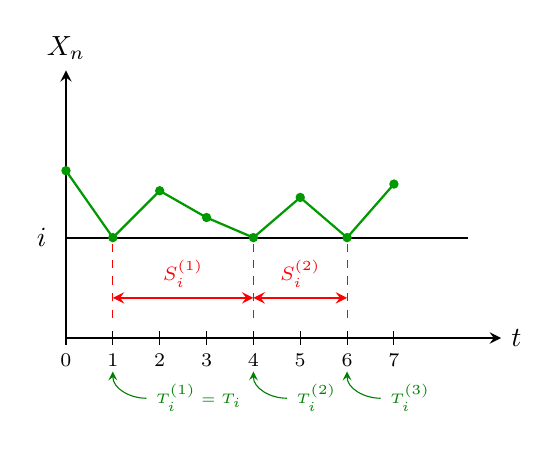
\begin{tikzpicture}[scale=0.85, >=stealth]
            % Ejes coordinados
            \draw[->, thick] (0,0) -- (6.5,0) node[right] {$t$};
            \draw[->, thick] (0,0) -- (0,4) node[above] {$X_n$};
            
            % Línea del estado bajo análisis i
            \draw[thick] (0,1.5) -- (6,1.5) node[at start, left] {$i$ \ };            
            % Puntos temporales en el eje t
            \foreach \x in {0,1,2,3,4,5,6,7} {
                \draw (\x*0.7, 0.1) -- (\x*0.7, -0.1) node[below, font=\scriptsize] {\x};
            }
            
            % Trayectoria de la cadena (línea continua con marcadores de estado)
            \draw[thick, green!60!black] 
                (0,2.5) -- (0.7*1,1.5) -- (0.7*2,2.2) -- (0.7*3,1.8) -- 
                (0.7*4,1.5) -- (0.7*5,2.1) -- (0.7*6,1.5) -- (0.7*7,2.3);
                
            \foreach \p in {(0,2.5), (0.7,1.5), (0.7*2,2.2), (0.7*3,1.8), (0.7*4,1.5), (0.7*5,2.1), (0.7*6,1.5), (0.7*7,2.3)} {
                \fill[green!60!black] \p circle (2pt);
            }
            
            % Intervalos de tiempo S^(n) representados en rojo
            \draw[red, <->, thick] (0.7, 0.6) -- (0.7*4, 0.6) node[midway, above, font=\scriptsize] {$S_i^{(1)}$};
            \draw[red, <->, thick] (0.7*4, 0.6) -- (0.7*6, 0.6) node[midway, above, font=\scriptsize] {$S_i^{(2)}$};
            
            % Líneas verticales de acotación para los intervalos S
            \draw[red, dashed] (0.7, 0.3) -- (0.7, 1.4);
            \draw[red, dashed] (0.7*4, 0.3) -- (0.7*4, 1.4);
            \draw[red, dashed] (0.7*6, 0.3) -- (0.7*6, 1.4);
            
            % Flechas inferiores indicadoras para los tiempos absolutos T^(n)
            \draw[green!50!black, <-, thin] (0.7, -0.5) to[out=-90, in=180] (1.2, -0.9) node[right, font=\tiny] {$T_i^{(1)} = T_i$};
            \draw[green!50!black, <-, thin] (0.7*4, -0.5) to[out=-90, in=180] (3.3, -0.9) node[right, font=\tiny] {$T_i^{(2)}$};
            \draw[green!50!black, <-, thin] (0.7*6, -0.5) to[out=-90, in=180] (4.7, -0.9) node[right, font=\tiny] {$T_i^{(3)}$};
        \end{tikzpicture}
        \end{center}
    \end{minipage}
\end{tabular}

\vspace{0.6cm}

\begin{lema}
    Para todo índice de visita $r \geq 2$, condicionado a la ocurrencia en tiempo finito de la visita previa ($T_i^{(r-1)} < \infty$), el intervalo de tiempo relativo $S_i^{(r)}$ es estadísticamente \textbf{independiente} de la historia pasada del proceso $\{X_m : m \leq T_i^{(r-1)}\}$. Asimismo, su distribución satisface la identidad de homogeneidad:
    \[
    P\big(S_i^{(r)} = n \ \big| \ T_i^{(r-1)} < \infty\big) = P_i(T_i = n)
    \]

\begin{proof}
    % //TODO: entender demostración
% Para demostrar la independencia y la distribución del intervalo relativo, realizamos la aplicación directa de la \textbf{Propiedad Fuerte de Markov}, fijando como tiempo de parada aleatorio el instante de la visita precedente, es decir, $T = T_i^{(r-1)}$.
% \begin{itemize}
%     \item Condicionado a que dicho hito ocurra en tiempo finito ($T < \infty$), sabemos con total certeza por la definición constructiva del tiempo de paso que el estado de la cadena en ese momento es exactamente $i$, lo que implica que $X_T = i$.
%     \item Invocando el Teorema de la Propiedad Fuerte de Markov, el proceso futuro reiniciado a partir de ese hito, denotado por la secuencia $(X_{T+m})_{m \geq 0}$, constituye una cadena de Markov legal y autónoma que opera bajo el vector de distribución inicial concentrado $\delta_i$ y se rige por la misma matriz de transiciones elementales $P$. Además, esta nueva secuencia es estrictamente independiente de la trayectoria histórica pasada $\{X_0, X_1, \dots, X_T\}$.
%     \item Evaluando la definición analítica del intervalo de recurrencia $S_i^{(r)}$ bajo este nuevo sistema de coordenadas temporales, observamos que equivale al número mínimo de pasos necesarios para que el proceso regenerado vuelva a intersectar el estado $i$:
%     \[
%     S_i^{(r)} = \inf\{m \geq 1 : X_{T+m} = i\} = T_i^{(r)} - T_i^{(r-1)}
%     \]
%     \item Como el proceso futuro $(X_{T+m})_{m \geq 0}$ inicia formalmente en el estado $i$ ($X_T = i$) y es una réplica exacta e independiente de la física de la cadena original, la variable $S_i^{(r)}$ se comporta estructuralmente como el tiempo de primer paso elemental ($T_i$) de una cadena que arranca desde el origen en el estado $i$. 
% \end{itemize}
% Por consiguiente, la medida de probabilidad de dicho intervalo relativo colapsa de forma idéntica en la distribución de primer retorno original $P_i(T_i = n)$, completando formalmente la demostración del lema.
\end{proof}
\end{lema}

\observacion{
    Para entender que significa
    \begin{equation*}
        P_i(T_i = n)
    \end{equation*}
    recordemos que la notación corta $P_i(\cdot)$ significa que obligamos a la cadena a empezar en el paso cero en el estado $i$ ($X_0 = i$), y $T_i$ es el tiempo del primer paso a ese estado $i$. Esa probabilidad significa que una cadena completamente nueva de fábrica, que arranca hoy en el estado $i$, tarde exactamente $n$ pasos en regresar al estado $i$ por primera vez.
}


\begin{definicion}[Número de Visitas a un Estado]
    Sea $(X_n)_{n \geq 0}$ una cadena de Markov. Se define la variable aleatoria discreta $V_i$, que cuantifica el \textbf{número total de visitas al estado $i$}, mediante la suma de funciones indicadoras a lo largo de toda la trayectoria infinita del proceso:
    \[
    V_i = \sum_{n=0}^{\infty} I_{\{X_n = i\}}
    \]
\end{definicion}

\begin{observacion}
    Haciendo uso de la linealidad del operador del valor esperado, el número esperado de visitas que realiza la cadena al estado $i$ equivale a la suma de las probabilidades marginales de ocupación:
    \[
    E(V_i) = E\left( \sum_{n=0}^{\infty} I_{\{X_n = i\}} \right) = \sum_{n=0}^{\infty} E\left[ I_{\{X_n = i\}} \right] = \sum_{n=0}^{\infty} P(X_n = i)
    \]
    Cuando asumimos que el proceso inicia con total certeza en dicho estado de referencia ($X_0 = i$), esta identidad se reduce de forma directa a la suma del término diagonal de las matrices de transición en $n$ pasos:
    \[
    E_i(V_i) = \sum_{n=0}^{\infty} P_i(X_n = i) = \sum_{n=0}^{\infty} P_{ii}^{(n)}
    \]
\end{observacion}


\begin{definicion}[Probabilidad de Retorno]
    La \textbf{probabilidad de retorno} $h_i$ se define como la medida de probabilidad de que la cadena regrese al estado de origen $i$ en algún instante de tiempo estrictamente positivo y finito:
    \[
    h_i = P_i(T_i < \infty)
    \]
    donde $T_i = \inf\{n \geq 1 : X_n = i\}$ representa el tiempo de primer paso al estado $i$.
\end{definicion}

\begin{lema}
    Para todo índice entero de visitas $r = 0, 1, 2, \dots$, la probabilidad de que la cadena de Markov visite el estado $i$ estrictamente más de $r$ veces, dado que inició en $i$, sigue una distribución geométrica de supervivencia gobernada por la potencia de la probabilidad de retorno:
    \[
    P_i(V_i > r) = h_i^r
    \]
    \textit{Nota aclaratoria estructural:} Recuerda que el $(r+1)$-ésimo tiempo absoluto de paso se construye de forma aditiva mediante $T_i^{(r+1)} = T_i^{(r)} + S_i^{(r+1)}$, donde $S_i^{(r+1)}$ representa el correspondiente intervalo de recurrencia relativo.

\begin{proof}
    % //TODO: entender demostración
    % Desglosamos la demostración utilizando el principio de inducción matemática sobre el número de visitas $r$, apoyándonos en la equivalencia de eventos sobre trayectorias:
    % \begin{itemize}
    %     \item Partiendo de la condición inicial $X_0 = i$, afirmar que el proceso realiza estrictamente más de $r$ visitas al estado $i$ ($V_i > r$) equivale exactamente a certificar que el $r$-ésimo tiempo absoluto de visita ocurre en tiempo finito, es decir: $\{V_i > r\} = \{T_i^{(r)} < \infty\}$.
    %     \item \textbf{Paso Base ($r = 0$):} Evaluando la identidad para el origen absoluto, el suceso se cumple de manera inmediata por certeza trivial de la condición inicial:
    %     \[
    %     P_i(V_i > 0) = P_i(T_i^{(0)} < \infty) = P_i(0 < \infty) = 1 = h_i^0
    %     \]
    %     \item \textbf{Paso Inductivo:} Supongamos como hipótesis de inducción que la relación se verifica de forma válida para un índice de visita fijo $r$, tal que $P_i(T_i^{(r)} < \infty) = h_i^r$. Evaluamos a continuación la probabilidad para el paso sucesivo $r + 1$:
    %     \[
    %     P_i(V_i > r + 1) = P_i\big( T_i^{(r+1)} < \infty \big) = P_i\left( \{ T_i^{(r)} < \infty \} \cap \{ S_i^{(r+1)} < \infty \} \right)
    %     \]
    %     Aplicando la definición clásica de probabilidad condicional para la intersección de estos sucesos históricos, obtenemos:
    %     \[
    %     = P_i\big( S_i^{(r+1)} < \infty \ \big| \ T_i^{(r)} < \infty \big) \cdot P_i\big( T_i^{(r)} < \infty \big)
    %     \]
    %     Haciendo uso del lema de los intervalos relativos (demostrado previamente mediante la aplicación de la Propiedad Fuerte de Markov en el tiempo de parada $T_i^{(r)}$), sabemos que el primer factor condicional se distribuye idénticamente a la probabilidad de primer retorno elemental $P_i(T_i < \infty) = h_i$. Sustituyendo este valor junto con nuestra hipótesis inductiva, concluimos:
    %     \[
    %     = h_i \cdot h_i^r = h_i^{r+1}
    %     \]
    % \end{itemize}
    % Por lo tanto, la relación geométrica queda formalmente demostrada para todo $r \geq 0$.
\end{proof}
\end{lema}

\section{Estados Recurrentes y Transitorios}

\begin{teo}[Dicotomía Fundamental de los Estados]
    Para todo estado $i \in S$ de una cadena de Markov, se satisface de forma estricta y excluyente una de las siguientes dos condiciones analíticas asintóticas:
    \begin{enumerate}
        \item Si $P_i(T_i < \infty) = 1$, entonces el estado $i$ es \textbf{recurrente} y la serie infinita de sus probabilidades de transición diagonal \textbf{DIVERGE}:
        \[
        \sum_{m=0}^{\infty} P_{ii}^{(m)} = \infty
        \]
        \item Si $P_i(T_i < \infty) < 1$, entonces el estado $i$ es \textbf{transitorio} y la serie infinita de sus probabilidades de transición diagonal \textbf{CONVERGE}:
        \[
        \sum_{m=0}^{\infty} P_{ii}^{(m)} < \infty
        \]
    \end{enumerate}
\begin{proof}
    Evaluamos de forma separada los dos comportamientos mutuamente excluyentes de la probabilidad de retorno $h_i = P_i(T_i < \infty)$:
    \begin{itemize}
        \item[\textbf{Caso i)}] Supongamos que la probabilidad de primer retorno es unitaria: $P_i(T_i < \infty) = 1$, lo que implica que $h_i = 1$. Evaluando el límite de la probabilidad acumulada de colas para el número de visitas obtenemos:
        \[ 
        P_i(V_i = \infty) = \lim_{r \to \infty} P_i(V_i > r) = \lim_{r \to \infty} h_i^r = \lim_{r \to \infty} 1^r = 1 
        \]
        Esto confirma que el estado $i$ es recurrente. Adicionalmente, aplicando la expansión lineal para el valor esperado de la variable, la serie de transiciones diagonales diverge:
        \[
        \sum_{m=0}^{\infty} P_{ii}^{(m)} = E_i(V_i) \overset{(*)}{=} \sum_{r=0}^{\infty} P_i(V_i > r) = \sum_{r=0}^{\infty} 1^r = \infty
        \]
        donde en $(*)$ hemos usado lo obtenido a continuación
        \begin{align*}
            E(X)& = \sum_{k=1}^{\infty} k \cdot P(X = k) \implies E(X) \overset{(**)}{=} \sum_{k=1}^{\infty} \left( \sum_{r=0}^{k-1} 1 \right) P(X = k) = \sum_{k=1}^{\infty} \sum_{r=0}^{k-1} P(X = k) \implies \\
            & \implies E(X) = \sum_{r=0}^{\infty} \sum_{k=r+1}^{\infty} P(X = k)= \sum_{r=0}^{\infty} P(X > r)
        \end{align*}
        donde en $(**)$ hemos utilizado que $k=\sum\limits_{r=0}^{k-1} 1$.
        
        \item[\textbf{Caso ii)}] Supongamos ahora que la probabilidad de primer retorno es estrictamente fraccionaria: $P_i(T_i < \infty) < 1$, de manera que $h_i < 1$. Al calcular de igual forma el comportamiento límite de la sucesión geométrica se deduce que:
        \[ 
        P_i(V_i = \infty) = \lim_{r \to \infty} P_i(V_i > r) = \lim_{r \to \infty} h_i^r = 0 
        \]
        Lo que define al estado $i$ como transitorio. Evaluando la esperanza matemática del número de visitas a través del sumatorio de su función de supervivencia, recuperamos de forma exacta la suma de una serie geométrica convergente de razón $h_i$:
        \[ 
        \sum_{m=0}^{\infty} P_{ii}^{(m)} = E_i(V_i) = \sum_{r=0}^{\infty} P_i(V_i > r) = \sum_{r=0}^{\infty} h_i^r = \frac{1}{1 - h_i} < \infty 
        \]
        Al ser $h_i < 1$, el denominador es estrictamente positivo, asegurando la convergencia finita de la serie de probabilidades, completando formalmente la demostración del teorema.
    \end{itemize}
\end{proof}
\end{teo}


\begin{teo}
    Para todo estado $i \in S$ de una cadena de Markov, se verifican las siguientes equivalencias fundamentales sobre el horizonte temporal finito:
    \begin{enumerate}
        \item Un estado $i$ es \textbf{recurrente} si y solo si $P_i(X_n = i \text{ para algún } n \geq 1) = 1$.
        \item Un estado $i$ es \textbf{transitorio} si y solo si $P_i(X_n = i \text{ para algún } n \geq 1) < 1$.
    \end{enumerate}

\begin{proof}
    %     % //TODO: entender demostración
    % Desglosamos las implicaciones lógicas para cada una de las dos afirmaciones de la dicotomía:

    % \subsection*{Demostración de la Afirmación 1}
    % \begin{itemize}
    %     \item[\textbf{($\implies$)}] Supongamos que el estado $i$ es recurrente. Dado que el evento de visitar el estado infinitas veces es un subconjunto estricto del evento que describe visitarlo al menos una vez en tiempo finito, podemos acotar superior e inferiormente la medida de probabilidad:
    %     \[ 
    %     1 = P_i(X_n = i \text{ i.v.}) \leq P_i(X_n = i \text{ para algún } n \geq 1) \leq 1 
    %     \]
    %     Por el teorema del sándwich, concluimos de forma inmediata que $P_i(X_n = i \text{ para algún } n \geq 1) = 1$.
        
    %     \item[\textbf{($\Longleftarrow$)}] Supongamos ahora que se cumple la condición de certeza para el primer retorno: $P_i(X_n = i \text{ para algún } n \geq 1) = 1$. Esto equivale por definición a afirmar que la probabilidad del tiempo de primer paso es finita: $P_i(T_i < \infty) = 1$. 
        
    %     Dado que $T_i$ constituye un \textbf{tiempo de parada}, invocamos la \textbf{Propiedad Fuerte de Markov} en dicho hito. El proceso futuro regenerado $Y_m = X_{T+m}$ es una cadena de Markov independiente que inicia en el estado $i$ y cumple formalmente que $P_i(Y_m = i \text{ para algún } m \geq 1) = 1$. Esto garantiza que el segundo tiempo absoluto de paso también ocurre con certeza en tiempo finito: $P_i(T_i^{(2)} < \infty) = 1$.
        
    %     Iterando inductivamente este argumento, demostramos que para todo índice de visita $l \geq 2$ se satisface que $P_i(T_i^{(l)} < \infty) = 1$. Al enlazar esta propiedad con la variable del número de visitas $V_i$, evaluamos el límite asintótico:
    %     \[ 
    %     P_i(V_i > l + 1) = P_i(T_i^{(l)} < \infty) = 1 \implies \lim_{l \to \infty} P_i(V_i > l + 1) = P_i(V_i = \infty) = 1 
    %     \]
    %     Al ser la probabilidad de realizar infinitas visitas igual a 1, queda demostrado que el estado $i$ es recurrente.
    % \end{itemize}

    % \subsection*{Demostración de la Afirmación 2}
    % \begin{itemize}
    %     \item[\textbf{($\Longleftarrow$)}] Supongamos que la probabilidad de retornar al menos una vez es estrictamente menor que la certeza: $P_i(X_n = i \text{ para algún } n \geq 1) = h_i < 1$. Bajo este escenario, la distribución geométrica de supervivencia del número de visitas calculada previamente nos asegura que la probabilidad de realizar infinitas visitas colapsa a cero, por lo que el número total de visitas es finito con probabilidad 1 ($P_i(V_i < \infty) = 1$). Por consiguiente, el estado $i$ es, por definición, transitorio.
        
    %     \item[\textbf{($\implies$)}] Demostraremos esta implicación mediante reducción al absurdo. Supongamos que el estado $i$ es transitorio pero que, contrariamente a lo enunciado, se cumpliera que $P_i(X_n = i \text{ para algún } n \geq 1) = 1$. Por el desarrollo analítico efectuado en la Demostración de la Afirmación 1 ($\Longleftarrow$), esta premisa nos forzaría a concluir que $P_i(X_n = i \text{ i.v.}) = 1$. Sin embargo, esto entra en contradicción directa con la hipótesis inicial de transitoriedad, la cual exige de forma estricta que $P_i(X_n = i \text{ i.v.}) = 0$. Por lo tanto, la suposición es falsa y se debe cumplir que $P_i(X_n = i \text{ para algún } n \geq 1) < 1$.
    % \end{itemize}
\end{proof}
\end{teo}




\begin{teo}[Propiedad de Solidaridad]
    La recurrencia y la transitoriedad son propiedades de clase. Es decir, dada una clase de comunicación $C$, o bien todos los estados pertenecientes a $C$ son transitorios, o bien todos los estados en $C$ son recurrentes. \\


\begin{proof}
    % //TODO: entender demostración
    % Sean $i, j \in C$ dos estados distintos que se comunican mutuamente ($i \longleftrightarrow j$). Supongamos, sin pérdida de generalidad, que el estado $i$ es transitorio. Por definición de comunicación, existen dos horizontes de pasos fijos $m, n \geq 0$ tales que las intensidades elementales de transición satisfacen que $P_{ij}^{(m)} > 0$ y $P_{ji}^{(n)} > 0$.

    % Para evaluar la dinámica del estado $j$, construimos una cota inferior para la probabilidad diagonal a pasos $m+l+n$ recurriendo a las ecuaciones de Chapman-Kolmogorov. Para cualquier número de pasos intermedios $l \geq 0$, la cadena puede efectuar la trayectoria específica $i \to j \to j \to i$, lo que nos permite asegurar la desigualdad:
    % \[ 
    % P_{ii}^{(m+l+n)} \geq P_{ij}^{(m)} P_{jj}^{(l)} P_{ji}^{(n)} 
    % \]

    % Dado que el producto de las transiciones de los extremos es estrictamente positivo ($P_{ij}^{(m)} P_{ji}^{(n)} > 0$), podemos despejar el término diagonal central $P_{jj}^{(l)}$ de la desigualdad como:
    % \[ 
    % P_{jj}^{(l)} \leq \frac{P_{ii}^{(m+l+n)}}{P_{ij}^{(m)} P_{ji}^{(n)}} 
    % \]

    % Aplicando el operador de sumatorio infinito en ambos lados de la relación para evaluar el número esperado de visitas, obtenemos:
    % \[ 
    % \sum_{l=0}^{\infty} P_{jj}^{(l)} \leq \frac{1}{P_{ij}^{(m)} P_{ji}^{(n)}} \sum_{l=0}^{\infty} P_{ii}^{(m+l+n)} 
    % \]

    % Por hipótesis, el estado $i$ es transitorio, lo que por el Teorema de Dicotomía garantiza que la serie completa de sus probabilidades diagonales converge: $\sum_{k=0}^{\infty} P_{ii}^{(k)} < \infty$. Como la cola de una serie convergente sigue siendo convergente, se verifica que $\sum_{l=0}^{\infty} P_{ii}^{(m+l+n)} < \infty$. 

    % Consecuentemente, la serie correspondiente al estado $j$ queda acotada superiormente por un valor real finito:
    % \[
    % \sum_{l=0}^{\infty} P_{jj}^{(l)} < \infty
    % \]
    % Esto demuestra que el estado $j$ es obligatoriamente transitorio. Si el estado $j$ fuese recurrente, la serie divergería a infinito, alcanzando una contradicción directa con la cota superior establecida.
\end{proof}
\end{teo}

\begin{teo}
    Toda clase de comunicación recurrente es matemáticamente cerrada.

\begin{proof}
    % //TODO: entender demostración
    % Supongamos, contrariamente a lo enunciado (reducción al absurdo), que existe una clase de comunicación $C$ que es recurrente pero que no es cerrada. Por definición de clase abierta, debe existir al menos un estado interno $i \in C$ y un estado externo $j \notin C$ tales que la cadena puede escapar de la clase en un número finito de pasos $m \geq 1$, es decir, $P_i(X_m = j) > 0$.

    % Analicemos el evento complementario de retorno. Si la cadena visita el estado externo en el paso $m$ ($X_m = j$), dado que $j$ no se comunica con $i$ ($j \not\to i$ por no pertenecer a la misma clase), la probabilidad de regresar al estado original $i$ en cualquier instante posterior es nula. Por lo tanto, la probabilidad conjunta de escapar hacia $j$ y visitar el origen infinitas veces colapsa a cero:
    % \[ 
    % P_i\big( \{X_m = j\} \cap \{X_n = i \text{ para infinitos } n\} \big) = 0 
    % \]

    % Utilizando la ley de la probabilidad total para descomponer la probabilidad de recurrencia global del estado $i$, deducimos:
    % \begin{align*}
    %     P_i(X_n = i \text{ i.v.}) &= P_i(X_n = i \text{ i.v.} \mid X_m = j) P_i(X_m = j) + P_i(X_n = i \text{ i.v.} \mid X_m \neq j) P_i(X_m \neq j) \\
    %     &= 0 + P_i(X_n = i \text{ i.v.} \mid X_m \neq j) P_i(X_m \neq j) \leq P_i(X_m \neq j)
    % \end{align*}

    % Como la probabilidad de escape es estrictamente positiva ($P_i(X_m = j) > 0$), la probabilidad del evento complementario es estrictamente menor que la certeza: $P_i(X_m \neq j) = 1 - P_i(X_m = j) < 1$. Por lo tanto:
    % \[
    % P_i(X_n = i \text{ infinitas veces}) < 1
    % \]
    % Esto contradice la hipótesis inicial de que la clase $C$ es recurrente (lo cual exige que todos sus estados regresen con probabilidad 1). Concluimos que la clase $C$ debe ser cerrada.
\end{proof}
\end{teo}


\begin{teo}
    Toda clase de comunicación que sea cerrada y finita es recurrente.

\begin{proof}
    %//TODO: entender demostración
    % Sea $C$ una clase cerrada y finita constituida por un número entero $K$ de estados, $C = \{i_1, i_2, \dots, i_K\}$. Asumamos que el proceso $(X_n)_{n \geq 0}$ inicia su trayectoria dentro de la clase ($X_0 \in C$). Dado que la clase es cerrada, la cadena jamás podrá abandonar esta región, lo que implica que con probabilidad 1:
    % \[
    % \sum_{j \in C} \sum_{n=0}^{\infty} \mathbb{I}_{\{X_n = j\}} = \infty
    % \]

    % Como estamos distribuyendo una cantidad infinita de visitas sobre un conjunto finito de $K$ estados, por el principio del palomar probabilístico es matemáticamente imposible que todos los estados de la clase sean transitorios. Si todos fuesen transitorios, cada uno recibiría únicamente un número finito de visitas con probabilidad 1, lo que contradice la hipótesis de permanencia permanente. 

    % Por lo tanto, debe existir al menos un estado de la clase, que denominaremos $j \in C$, que sea visitado infinitas veces con probabilidad positiva:
    % \[
    % P(X_n = j \text{ infinitas veces} \mid X_0 = i) > 0
    % \]
    % Al no ser su probabilidad de retorno nula, el estado $j$ no puede ser transitorio, categorizándose como recurrente. Finalmente, invocando el Teorema de Solidaridad de clases demostrado previamente, al ser $j$ recurrente, todos los demás estados que comparten la clase de comunicación $C$ son obligatoriamente recurrentes.
\end{proof}
\begin{proof}[Demostración Alternativa Analítica]
    % //TODO: entender demostración
    % Fijemos un estado de partida $i \in C$. Como la clase es finita y cerrada, la masa de probabilidad total se concentra en sus estados a largo plazo, garantizando que existe al menos un estado $j \in C$ tal que $P_i(X_n = j \text{ i.v.}) > 0$. Adicionalmente, como $i$ y $j$ pertenecen a la misma clase de comunicación, se comunican mutuamente, por lo que existe un horizonte $m \geq 0$ tal que $P_{ji}^{(m)} > 0$.

    % Evaluamos la probabilidad de recurrencia del estado $j$ condicionando su trayectoria a través del estado intermedio $i$:
    % \[ 
    % P_j(X_n = j \text{ infinitas veces}) \geq P_{ji}^{(m)} \, P_i(X_n = j \text{ infinitas veces}) 
    % \]
    % Dado que ambos factores del extremo derecho son estrictamente mayores que cero por hipótesis ($P_{ji}^{(m)} > 0$ y $P_i(X_n = j \text{ i.v.}) > 0$), el producto resulta ser estrictamente positivo:
    % \[
    % P_j(X_n = j \text{ infinitas veces}) > 0
    % \]
    % Por la dicotomía fundamental de los estados, la probabilidad de visitar un estado infinitas veces solo puede adoptar los valores puros de 0 o 1. Al haber demostrado que es estrictamente mayor que 0, se concluye que obligatoriamente debe ser igual a 1, clasificando al estado $j$ como recurrente y contagiando dicha propiedad a toda la clase $C$.
\end{proof}

\end{teo}

\begin{coro}
    Si $(X_n)_{n \geq 0}$ es una cadena de Markov que opera sobre un espacio de estados de carácter finito ($|S| < \infty$), entonces se satisfacen de forma exacta las siguientes equivalencias estructurales fundamentales:
    \begin{enumerate}
        \item Una clase de comunicación es \textbf{cerrada} si y solo si es \textbf{recurrente}.
        \item Una clase de comunicación \textbf{no es cerrada} si y solo si es \textbf{transitoria}.
    \end{enumerate}
\end{coro}


\begin{ejemplo}[Grafo Dinámico de la Marcha Aleatoria en $\mathbb{Z}$]
Considere una marcha aleatoria simple que evoluciona sobre el conjunto infinito de los números enteros. Las probabilidades locales de transición asociadas a un estado genérico $i \in \mathbb{Z}$ vienen dadas, para un parámetro fijo $p \in (0,1)$, por el siguiente comportamiento dinámico:
\[ 
P_{i, i+1} = p, \qquad P_{i, i-1} = 1 - p 
\]

La representación esquemática del balance local de flujos de probabilidad de salto hacia los estados inmediatamente adyacentes se puede visualizar mediante el siguiente grafo unidimensional regulado en TikZ:

\begin{center}
    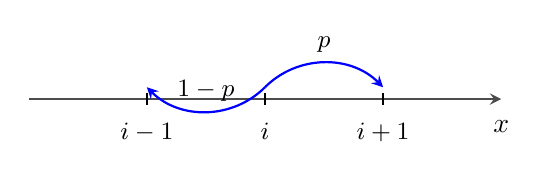
\begin{tikzpicture}[scale=1.5, >=stealth, semithick]
        % Eje graduado de base espacial
        \draw[->, thick, black!70] (-2,0) -- (2,0) node[below=4pt, black] {$x$};
        
        % Marcas y etiquetas de los estados locales
        \draw (-1,0.05) -- (-1,-0.05) node[below=3pt, font=\small] {$i-1$};
        \draw (0,0.05) -- (0,-0.05) node[below=3pt, font=\small] {$i$};
        \draw (1,0.05) -- (1,-0.05) node[below=3pt, font=\small] {$i+1$};
        
        % Flechas curvadas simétricas de transición probabilística
        \draw[->, blue, thick] (0,0.1) to[bend left=45] node[above, black, font=\small] {$p$} (1,0.1);
        \draw[->, blue, thick] (0,0.1) to[bend left=45] node[above, black, font=\small] {$1-p$} (-1,0.1);
    \end{tikzpicture}
\end{center}
\end{ejemplo}

\begin{teo}
    Sea $(Y_n)_{n \geq 0}$ una marcha aleatoria simple en $\mathbb{Z}$ con probabilidad de salto a la derecha dada por $p$. Se verifica la siguiente dicotomía fundamental para el espacio de estados:
    \begin{enumerate}
        \item Si $p \neq \frac{1}{2}$, entonces cada estado del espacio es \textbf{transitorio}.
        \item Si $p = \frac{1}{2}$, entonces cada estado del espacio es \textbf{recurrente}.
    \end{enumerate}

\begin{proof}
    % //TODO: entender demostración
    % Dado que el proceso cuenta con la propiedad de invariancia por traslación espacial, las propiedades probabilísticas dinámicas de cualquier estado son idénticas. Por consiguiente, podemos centrar nuestro estudio analítico en el estado origen $i = 0$.

    % Definimos la trayectoria de la marcha aleatoria mediante la suma acumulada de saltos locales:
    % \[ 
    % Y_n = \sum_{j=1}^{n} X_j, \qquad Y_0 = 0 
    % \]
    % donde las variables aleatorias $(X_j)_{j \geq 1}$ son independientes e idénticamente distribuidas (\textit{i.i.d.}), modeladas bajo una distribución de Rademacher:
    % \[ 
    % X_j = \begin{cases} +1 & \text{con prob. } p \\ -1 & \text{con prob. } 1-p \end{cases} 
    % \]
    % Si consideramos una variable aleatoria de Bernoulli estándar $\widetilde{X} \sim \text{Ber}(p)$, podemos mapear linealmente el soporte de los saltos mediante la transformación algebraica $X = 2\widetilde{X} - 1$. Haciendo uso de la linealidad del operador esperanza, calculamos el primer momento de los saltos individuales:
    % \[ 
    % E[X_1] = E[2\widetilde{X} - 1] = 2 E[\widetilde{X}] - 1 = 2p - 1 
    % \]

    % Dividimos el desarrollo analítico en los dos escenarios excluyentes gobernados por el parámetro $p$:

    % \subsection*{Caso 1: Marcha Aleatoria Sesgada ($p \neq \frac{1}{2}$)}
    % Al cumplirse que $p \neq \frac{1}{2}$, la esperanza matemática del salto es estrictamente no nula ($E[X_1] = 2p - 1 \neq 0$). Invocando la \textbf{Ley Fuerte de los Grandes Números (LFGN)}, la media muestral de las transiciones converge con certeza casi segura (\textit{c.s.}) hacia su media teórica:
    % \[ 
    % P\left( \lim_{m \to \infty} \frac{1}{m} \sum_{i=1}^{m} X_i = 2p - 1 \right) = 1 
    % \]
    % Esto nos permite aproximar de manera asintótica el valor de la posición absoluta de la cadena en el paso $m$ como:
    % \[ 
    % Y_m \overset{\text{c.s.}}{\approx} m(2p - 1) 
    % \]
    % Evaluando el comportamiento límite de la trayectoria cuando el horizonte temporal tiende al infinito, deducimos un comportamiento divergente forzado por el signo del sesgo:
    % \[ 
    % \lim_{m \to \infty} Y_m \overset{\text{c.s.}}{=} \begin{cases} +\infty & \text{si } p > \frac{1}{2} \\ -\infty & \text{si } p < \frac{1}{2} \end{cases} 
    % \]
    % Dado que la trayectoria escapa de forma definitiva hacia los extremos infinitos del eje real con probabilidad 1, el proceso solo puede regresar al origen un número finito de veces. Consecuentemente, la probabilidad límite colapsa a cero:
    % \[ 
    % P_0(Y_m = 0 \text{ infinitas veces}) = 0 
    % \]
    % Lo que clasifica formalmente al estado de referencia $Y_0 = 0$ como un \textbf{estado transitorio}.

    % \subsection*{Caso 2: Marcha Aleatoria Simétrica ($p = \frac{1}{2}$)}
    % Cuando la probabilidad está perfectamente equilibrada, la probabilidad de transición diagonal en $m$ pasos ($P_{00}^{(m)}$) depende estrictamente de la paridad del paso debido al carácter bipartito del retículo:
    % \[ 
    % P_{00}^{(m)} = \begin{cases} 0 & \text{si } m = 2k+1 \\ \dfrac{1}{2^{2k}} \dbinom{2k}{k} & \text{si } m = 2k \end{cases} 
    % \]
    % Para evaluar el criterio de recurrencia mediante la serie de transiciones de ocupación $\sum_{m=0}^{\infty} P_{00}^{(m)}$, aproximamos el comportamiento asintótico del término combinatorio factorial para un horizonte lejano ($k \gg 1$) empleando la \textbf{Fórmula de Stirling} ($m! \sim \sqrt{2\pi m} (m/e)^m$):
    % \[ 
    % P_{00}^{(2k)} = \frac{(2k)!}{k! \, k!} \frac{1}{2^{2k}} \sim \frac{\sqrt{4\pi k} \left(\frac{2k}{e}\right)^{2k}}{\left[\sqrt{2\pi k} \left(\frac{k}{e}\right)^k\right]^2} \frac{1}{2^{2k}} = \frac{2\sqrt{\pi k} \cdot 2^{2k} \cdot k^{2k} e^{-2k}}{2\pi k \cdot k^{2k} e^{-2k}} \frac{1}{2^{2k}} = \frac{1}{\sqrt{\pi k}} 
    % \]

    % Evaluando la convergencia de la serie mediante este equivalente asintótico, expandimos los términos:
    % \[ 
    % \sum_{m=0}^{\infty} P_{00}^{(m)} = \sum_{k=0}^{\infty} P_{00}^{(2k)} \sim \frac{1}{\sqrt{\pi}} \sum_{k=1}^{\infty} \frac{1}{k^{1/2}} 
    % \]
    % Haciendo uso de los criterios estándar de convergencia de series de potencias reales (sabiendo que la serie armónica $\sum k^{-1} = \infty$ y que las $p$-series con exponente menor o igual a la unidad divergen, $\sum k^{-1/2} = \infty$), determinamos que la suma total diverge:
    % \[ 
    % \sum_{m=0}^{\infty} P_{00}^{(m)} = \infty 
    % \]
    % Por el Teorema Fundamental de Dicotomía, al diverger el número esperado de visitas, el estado de origen $0$ es formalmente \textbf{recurrente}.
\end{proof}

\end{teo}

\begin{observacion}[Efecto de la Dimensión en la Recurrencia]
    Como conclusión estructural de este análisis de marchas aleatorias, se desprende que cualquier marcha sesgada (\textit{biased}) es siempre transitoria, mientras que la marcha no sesgada o simétrica (\textit{unbiased}) conserva su carácter recurrente sobre los retículos de dimensiones $d=1$ y $d=2$. No obstante, en virtud del Teorema de Polya, para cualquier retículo cúbico hiperbólico de dimensión tres o superior ($d \geq 3$), la marcha aleatoria simétrica se vuelve estrictamente \textbf{transitoria}.
\end{observacion}


\begin{definicion}[Variables de Ocupación antes del Retorno]
    Sea $(X_n)_{n \geq 0}$ una cadena de Markov que evoluciona sobre un espacio de estados arbitrario $E$. Fijado un estado de referencia base $k \in E$, definimos el tiempo de primera llegada como la variable aleatoria:
    \[ 
    T_k = \inf\{n \geq 1 : X_n = k\} \in \mathbb{N} \cup \{\infty\} 
    \]
    A partir de este hito temporal, se define la variable estadística $\gamma_i^{(k)}$ como el \textbf{número esperado de visitas realizadas al estado $i$ antes de que la cadena regrese por primera vez al estado original $k$}:
    \[ 
    \gamma_i = \gamma_i^{(k)} = E_k \left( \sum_{n=0}^{T_k - 1} I_{\{X_n = i\}} \right) \in [0, +\infty] 
    \]
    donde hemos usado que $E_k(\cdot) \equiv E(\cdot \mid X_0 = k) $.
\end{definicion}



\begin{teo}[Teorema de existencia general de medida invariante]
    Para una cadena de Markov irreducible y recurrente que comienza su trayectoria en el estado de referencia $k \in E$, la medida del número esperado de visitas intermedias $\gamma = (\gamma_i)_{i \in E}$ cumple rigurosamente las siguientes tres propiedades estructurales:
    \begin{enumerate}
        \item $\gamma_k = \gamma_k^{(k)} = 1$
        \item Para todo estado $i \in E$, el valor está estrictamente acotado: $0 < \gamma_i < \infty$.
        \item El vector $\gamma = (\gamma_i)_{i \in E}$ constituye una \textbf{medida invariante} del sistema, es decir
        \begin{equation*}
            \gamma P =\gamma
        \end{equation*}
    \end{enumerate}

\begin{proof}
    Desglosamos la verificación analítica para cada uno de los tres apartados del teorema:
    \begin{description}
        \item[$(1)$] Por definición constructiva de la variable aleatoria de ocupación, evaluamos la esperanza de la suma indicadora partiendo del estado $k$:
            \[ 
            \gamma_k = E_k \left( \sum_{m=0}^{T_k - 1} I_{\{X_m = k\}} \right) 
            \]
            Dado que el proceso arranca con certeza en $k$ ($X_0 = k$), la primera indicadora toma el valor de 1. Para cualquier instante de tiempo posterior $1 \leq m \leq T_k - 1$, por la propia definición matemática del tiempo de primer retorno ($T_k = \inf\{n \geq 1 : X_n = k\}$), la cadena tiene estrictamente prohibido regresar a $k$. Por lo tanto, el sumatorio se reduce únicamente a su término inicial:
            \[
            \gamma_k = E_k(I_{\{X_0 = k\}}) = E_k(1) = 1
            \]
        \item[$(3)$] Para demostrar analíticamente que $\gamma$ es una medida invariante bajo la acción de la matriz de transición, debemos verificar el cumplimiento exacto de la ecuación algebraico-lineal de balance para cualquier estado de destino $j \in E$:
            \[
            \gamma_j = \sum_{i \in E} \gamma_i P_{ij}
            \]
            Dado que la hipótesis del teorema nos asegura que la cadena es recurrente, el tiempo de primer retorno ocurre de forma finita casi con total certeza ($T_k < \infty$ c.s.), lo que implica la identidad de fronteras $X_0 = k = X_{T_k}$. Mediante un desplazamiento cíclico del índice temporal, alteramos los extremos del sumatorio interior:
            \[
            \gamma_j = E_k \left( \sum_{m=0}^{T_k - 1} I_{\{X_m = j\}} \right) 
            = E_k \left( \sum_{m=1}^{T_k} I_{\{X_m = j\}} \right) 
            \]
            Extendiendo el sumatorio formalmente hacia el horizonte infinito mediante la introducción de la condición indicadora $\{m \leq T_k\}$ y explotando la linealidad del operador valor esperado, desarrollamos:
            \[
            = E_k \left( \sum_{m=1}^{\infty} I_{\{X_m = j, \, m \leq T_k\}} \right) 
            = \sum_{m=1}^{\infty} E_k \left( I_{\{X_m = j, \, m \leq T_k\}} \right) 
            = \sum_{m=1}^{\infty} P_k (X_m = j, \, m \leq T_k)
            \]
            Aplicamos el Teorema de la Probabilidad Total introduciendo una partición exhaustiva sobre el espacio de estados intermedios visitados en el paso temporal inmediatamente anterior $X_{m-1} = i$, pues si sumamos la probabilidad de transición desde todos los estados posibles $i \in E$, obtenemos la probabilidad total de alcanzar el estado $j$ en el paso $m$
            \[
            = \sum_{i \in E} \sum_{m=1}^{\infty} P_k (X_m = j, \, X_{m-1} = i, \, T_k \geq m)
            \]
            Invocando la \textbf{Propiedad de Markov} ordinaria, el comportamiento dinámico del paso $m$ se desvincula de las restricciones históricas del pasado acumuladas en el evento $\{T_k \geq m\}$, es decir, aplicando esto en $(**)$ y la probabilidad condicionada en $(*)$ tenemos

            \begin{align*}
                P_k (X_m = j, \, X_{m-1} = i, \, T_k \geq m) &\overset{(*)}{=} P_k (X_m = j \mid X_{m-1} = i, \, T_k \geq m) \, P_k (X_{m-1} = i, \, T_k \geq m) =\\
                &\overset{(**)}{=} P_k (X_m = j \mid X_{m-1} = i) \, P_k (X_{m-1} = i, \, T_k \geq m)
            \end{align*}
            y aplicando la homogeneidad temporal tenemos
            \[
            \gamma_j=\sum_{i \in E} \sum_{m=1}^{\infty} P_{ij} \, P_k (X_{m-1} = i, \, T_k \geq m)
            \]
            Efectuamos un cambio de variable elemental sobre el índice temporal de la serie interior fijando $m' = m - 1$:
            \[
            = \sum_{i \in E} \sum_{m'=0}^{\infty} P_{ij} \, P_k (X_{m'} = i, \, T_k \geq m' + 1)
            \]
            Restaurando la variable indicadora dentro de la esperanza matemática y traduciendo la condición de cota superior $\{T_k \geq m + 1\}$ como $\{T_k - 1 \geq m\}$, la igualdad de balance se consolida al reagrupar los términos:
            \[
            = \sum_{i \in E} \sum_{m=0}^{\infty} P_{ij} \, E_k \left( I_{\{X_m = i, \, T_k \geq m + 1\}} \right) 
            = \sum_{i \in E} P_{ij} \, \underbrace{E_k \left( \sum_{m=0}^{T_k - 1} I_{\{X_m = i\}} \right)}_{\gamma_i} 
            = \sum_{i \in E} \gamma_i P_{ij}
            \]
            Por lo tanto, queda formalmente demostrado que el vector $\gamma$ constituye una medida invariante de la cadena.
        \item[$(2)$] Debido a la hipótesis de irreducibilidad del sistema, sabemos que todos los estados se comunican libremente entre sí. Por consiguiente, fijado un estado arbitrario $i \in E$, se garantiza de forma deductiva la existencia de dos horizontes de pasos finitos $m, n \geq 0$ tales que las probabilidades de transición en múltiples pasos satisfacen que $P_{ki}^{(m)} > 0$ y $P_{ik}^{(n)} > 0$.

            Haciendo uso de la propiedad de invarianza de la medida demostrada en el apartado anterior ($\gamma = \gamma P^m$), desglosamos el sumatorio matricial para aislar la contribución del estado de referencia $k$:
            \[ 
            \gamma_i = \sum_{j \in E} \gamma_j P_{ji}^{(m)} \geq \gamma_k P_{ki}^{(m)} 
            \]
            Sustituyendo el valor unitario de la frontera obtenido en el primer apartado ($\gamma_k = 1$), establecemos la acotación inferior estricta:
            \[
            \gamma_i \geq (1) \cdot P_{ki}^{(m)} = P_{ki}^{(m)} > 0
            \]
            Para verificar la cota superior, evaluamos de igual forma la invarianza de la medida sobre el estado $k$ tras un horizonte de $n$ pasos ($\gamma = \gamma P^n$), aislando en esta ocasión el aporte del estado intermedio $i$:
            \[ 
            1 = \gamma_k = \sum_{j \in E} \gamma_j P_{jk}^{(n)} \geq \gamma_i P_{ik}^{(n)} 
            \]
            Despejando el término de interés, dado que la intensidad de transición es estrictamente positiva ($P_{ik}^{(n)} > 0$), la componente queda confinada superiormente por un valor real real finito:
            \[ 
            \gamma_i \leq \frac{1}{P_{ik}^{(n)}} < \infty 
            \]
            Al haber demostrado que la componente es estrictamente positiva y finita para cualquier estado del espacio, se completa la demostración de todas las tesis del teorema.
    \end{description} 
\end{proof}
\end{teo}

\begin{teo}[Teorema del núcleo fundamental de medida invariante]
    Sea $(X_n)_{n \geq 0}$ una cadena de Markov irreducible y recurrente que opera sobre un espacio de estados discreto $E$. Fijemos un estado arbitrario de referencia $k \in E$. Entonces, cualquier medida invariante $\lambda = (\lambda_j)_{j \in E}$ asociada al sistema es única salvo por un factor de proporcionalidad constante. Es decir, se puede escribir de forma unívoca como:
    \[ 
    \lambda_j = c \gamma_j^{(k)} \qquad \forall j \in E 
    \]
    donde la constante multiplicativa viene dada por la masa del estado de referencia, $c = \lambda_k$, la cual es estrictamente independiente del estado de destino $j$.

\begin{proof}
    % //TODO: entender demostración
    % Sea $\lambda$ una medida invariante arbitraria del sistema que satisface las ecuaciones lineales de balance $\lambda = \lambda P$. Demostraremos en primera instancia la desigualdad fundamental $\lambda_j \geq \lambda_k \gamma_j^{(k)}$ mediante un procedimiento de expansión iterativo por caminos condicionales.

    % Descomponemos recursivamente el sumatorio de la ecuación de invarianza para el estado $j$, aislando en cada etapa el aporte del estado de referencia $k$ respecto al resto de la región complementaria $i \neq k$:
    % \begin{align*}
    %     \lambda_j &= \sum_{i_0 \in E} \lambda_{i_0} P_{i_0 j} = \sum_{i_0 \neq k} \lambda_{i_0} P_{i_0 j} + \lambda_k P_{kj} \\
    %     &= \sum_{i_0 \neq k} \left( \sum_{i_1 \neq k} \lambda_{i_1} P_{i_1 i_0} + \lambda_k P_{k i_1} \right) P_{i_0 j} + \lambda_k P_{kj} \\
    %     &= \sum_{i_0 \neq k} \sum_{i_1 \neq k} \lambda_{i_1} P_{i_1 i_0} P_{i_0 j} + \lambda_k P_{kj} + \lambda_k \sum_{i_0 \neq k} P_{k i_0} P_{i_0 j}
    % \end{align*}

    % Reiterando este proceso de sustitución inductiva hacia atrás un número finito de $m$ pasos, la estructura algebraica adopta la siguiente forma generalizada por sumas de trayectorias truncadas:
    % \[ 
    % \lambda_j = \sum_{i_0, \dots, i_m \neq k} \lambda_{i_m} P_{i_m i_{m-1}} \dots P_{i_1 i_0} P_{i_0 j} + \lambda_k \left( P_{kj} + \sum_{i_0 \neq k} P_{k i_0} P_{i_0 j} + \dots + \sum_{i_0, \dots, i_{m-1} \neq k} P_{k i_0} \dots P_{i_{m-1} j} \right) 
    % \]

    % Dado que todas las componentes del vector $\lambda$ y las celdas de la matriz de transición $P$ son no negativas, el sumatorio múltiple residual de la izquierda es estrictamente mayor o igual a cero. Al descartar dicho término sobrante, podemos fijar una cota inferior reconociendo que cada sumatorio entre paréntesis modela la probabilidad de una trayectoria elemental que arranca en $k$, visita estados fuera de $k$, y aterriza en $j$ exactamente en el paso correspondiente sin haber retornado antes a $k$:
    % \[ 
    % \Rightarrow \lambda_j \geq \lambda_k P_k [X_1 = j, T_k \geq 1] + \lambda_k P_k [X_2 = j, T_k \geq 2] + \dots + \lambda_k P_k [X_m = j, T_k \geq m] 
    % \]
    % Compactando esta suma finita de probabilidades marginales de trayectorias permitidas mediante un operador sumatorio, obtenemos la desigualdad válida para cualquier entero finito $m$:
    % \[ 
    % \lambda_j \geq \lambda_k \sum_{i=1}^{m} P_k [X_i = j, T_k \geq i] 
    % \]

    % Tomando el límite matemático cuando el horizonte de pasos tiende a infinito ($m \to \infty$) en ambos extremos de la desigualdad, la serie infinita se puede reescribir mediante la introducción del operador de la función indicadora dentro del valor esperado:
    % \[ 
    % \lambda_j \geq \lambda_k \sum_{m=1}^{\infty} P_k [X_m = j, T_k \geq m] = \lambda_k \sum_{m=1}^{\infty} E \left[ \mathbb{I}_{\{X_m = j, \, T_k \geq m\}} \right] 
    % \]
    % Haciendo uso de la linealidad de la esperanza y desplazando los límites por indexación temporal, la suma de las variables indicadoras reconstruye de manera exacta la definición de la medida de ocupación intermedia $\gamma_j^{(k)}$ demostrada en la sección previa:
    % \[ 
    % \lambda_j \geq \lambda_k E_k \left[ \sum_{m=0}^{T_k - 1} \mathbb{I}_{\{X_m = j\}} \right] = \lambda_k \gamma_j^{(k)} 
    % \]

    % De este modo, queda verificado de forma robusta que cualquier medida invariante cumple la cota inferior $\lambda_j \geq \lambda_k \gamma_j^{(k)}$. Para consolidar la igualdad estricta, se recurre a la propiedad de invarianza de la propia medida sobre el estado de referencia, completando formalmente la unicidad salvo constante multiplicativa de la medida.
\end{proof}
\end{teo}


\begin{observacion}
    Como consecuencia directa de este teorema, se establece que una cadena de Markov que es simultáneamente irreducible y recurrente posee una \textbf{única medida invariante} salvo por un factor de escala constante multiplicativo. Dependiendo de las propiedades de sumabilidad de la trayectoria, esta medida invariante única puede adoptar una masa total finita ($\sum \lambda_i < \infty$, caso recurrente positivo) o bien una masa total infinita ($\sum \lambda_i = \infty$, caso recurrente nulo).
\end{observacion}


\begin{coro}
    Toda cadena de Markov que sea irreducible y opere sobre un espacio de estados finito posee una \textbf{única medida de probabilidad invariante}.
\begin{proof}
    Desglosamos la verificación analítica en dos fases fundamentales: la construcción de una medida normalizada (de probabilidad) y la demostración formal de su unicidad.
    \begin{description}
        \item[\tbf{Fase 1.}] Por resultados previos del temario, sabemos que toda cadena de Markov que es simultáneamente cerrada (por ser irreducible) y finita cumple de forma obligatoria con la condición de ser \textbf{recurrente}.

    Al haber demostrado la recurrencia, podemos invocar el teorema de existencia general, el cual nos garantiza que existe una medida invariante $\lambda = (\lambda_i)_{i \in E}$ que es única salvo por una constante multiplicativa escalar. Además, sabemos que todos sus componentes son estrictamente positivos y reales ($\lambda_i > 0$).

    \begin{enumerate}
        \item \textbf{Finitud de la masa total:} 
        Dado que el espacio de estados $E$ es estrictamente \textbf{finito}, podemos asegurar con total rigor matemático que la suma de todos los componentes de la medida $\lambda$ no diverge. Definimos esta masa total como la constante $M$:
        \[
        M = \sum_{i \in E} \lambda_i < \infty
        \]
        Si el espacio $E$ fuese infinito, esta suma podría divergir a infinito, impidiendo el proceso de normalización.
        
        \item \textbf{Construcción de la medida de probabilidad ($\lambda'$):}
        Para transformar nuestra medida general $\lambda$ en una medida de probabilidad (cuya suma total sea exactamente $1$), procedemos a dividir cada componente individual por la masa total $M$. Definimos algebraicamente este nuevo vector como $\lambda'$ (``lambda prima''):
        \[
        \lambda'_i = \frac{\lambda_i}{M} \quad \forall i \in E
        \]
        
        \item \textbf{Verificación del axioma de probabilidad:}
        Haciendo uso de la linealidad del operador sumatorio, verificamos analíticamente que $\lambda'$ distribuye una masa de probabilidad unitaria sobre todo el espacio:
        \[
        \sum_{i \in E} \lambda'_i = \sum_{i \in E} \frac{\lambda_i}{M} = \frac{1}{M} \sum_{i \in E} \lambda_i = \frac{1}{M} \cdot M = 1
        \]
        Dado que $\lambda P = \lambda$, por linealidad se cumple inmediatamente que $\lambda' P = \lambda'$, consolidando a $\lambda'$ como una medida de probabilidad invariante legítima.
    \end{enumerate}

    \item[\tbf{Fase 2.}] Para demostrar que no puede existir otra medida de probabilidad invariante distinta, utilizaremos el método directo de reducción analítica por igualación de constantes. \\

    \noindent
    Supongamos hipotéticamente que existen dos medidas de probabilidad invariantes del sistema, a las que denominaremos $\nu'$ y $\nu''$. Fijemos un estado arbitrario de referencia $k \in E$.

    \begin{enumerate}
        \item \textbf{Relación con el vector de visitas esperadas ($\gamma^{(k)}$):}
        Por el teorema del núcleo fundamental, cualquier medida invariante del sistema debe ser un múltiplo escalar del vector fundamental de visitas intermedias esperado $\gamma^{(k)} = (\gamma_i^{(k)})_{i \in E}$. Consiguientemente, deben existir dos constantes reales estrictamente positivas $c'$ y $c''$ tales que:
        \[
        \nu'_i = c' \gamma_i^{(k)} \quad \text{y} \quad \nu''_i = c'' \gamma_i^{(k)} \quad \forall i \in E
        \]
        
        \item \textbf{Aplicación de la condición de normalización:}
        Como por hipótesis tanto $\nu'$ como $\nu''$ son medidas de probabilidad, la suma de sus componentes sobre el espacio exhaustivo $E$ debe ser idéntica a la unidad. Expandiendo ambas series mediante sustitución, obtenemos:
        \begin{align*}
            1 &= \sum_{i \in E} \nu'_i = \sum_{i \in E} c' \gamma_i^{(k)} = c' \sum_{i \in E} \gamma_i^{(k)} \\
            1 &= \sum_{i \in E} \nu''_i = \sum_{i \in E} c'' \gamma_i^{(k)} = c'' \sum_{i \in E} \gamma_i^{(k)}
        \end{align*}
        
        \item \textbf{Colapso e igualdad de constantes:}
        Despejando algebraicamente de forma directa los escalares $c'$ y $c''$ de las ecuaciones de balance anteriores, observamos que quedan unívocamente determinados por el mismo valor numérico real:
        \[
        c' = \frac{1}{\sum_{i \in E} \gamma_i^{(k)}} \quad \text{y} \quad c'' = \frac{1}{\sum_{i \in E} \gamma_i^{(k)}}
        \]
        Por transitividad algebraica, se deduce de forma inmediata que:
        \[
        c' = c''
        \]
        
        \item \textbf{Conclusión:}
        Al ser los escalares idénticos ($c' = c''$), los vectores constituyentes se igualan componente a componente para todo el espacio:
        \[
        \nu'_i = c' \gamma_i^{(k)} = c'' \gamma_i^{(k)} = \nu''_i \implies \nu' = \nu''
        \]
        Queda formalmente demostrado que cualquier medida de probabilidad invariante alternativa colapsa necesariamente en la misma estructura vector-espacio, confirmando la estricta unicidad de la solución.
    \end{enumerate}
    \end{description} 
\end{proof}
\end{coro}

\observacion{
La discrepancia fundamental entre \tbf{medida invariante} y \tbf{medida invariante de probabilidad} radica única y exclusivamente en la \textbf{masa total} del sistema (la suma de sus componentes), lo cual determina su interpretación matemática y su aplicabilidad en Data Science:
    \begin{itemize}
        \item \textbf{Medida Invariante ($\gamma$):} Es un vector de pesos no negativos que satisface la ecuación de balance algebraico $\gamma P = \gamma$. Su masa total es arbitraria y puede ser finita o infinita, es decir:
        \[
        M = \sum_{i \in E} \gamma_i \in (0, \infty]
        \]
        No representa probabilidades directas, sino proporciones relativas de tiempo o visitas esperadas entre los estados.
        
        \item \textbf{Medida de Probabilidad Invariante ($\pi$):} Es un caso particular de medida invariante ($\pi P = \pi$) que cumple estrictamente con los axiomas de Kolmogorov. Exige obligatoriamente que la masa total esté normalizada a la unidad:
        \[
        \sum_{i \in E} \pi_i = 1
        \]
        Permite una interpretación estadística asintótica directa (probabilidad de hallar a la cadena en el estado $i$ en un horizonte temporal lejano, $n \to \infty$).
    \end{itemize}
}

\begin{observacion}
    Si el espacio de estados $E$ es \textbf{finito}, toda medida invariante $\gamma$ posee una masa total finita ($M < \infty$), lo que garantiza que siempre se puede construir su correspondiente medida de probabilidad mediante el operador de normalización lineal $\pi_i = \frac{\gamma_i}{M}$. Si el espacio $E$ es infinito, la suma puede divergir ($M = \infty$), imposibilitando dicha normalización (cadenas recurrentes nulas).
\end{observacion}

\observacion{
    Este corolario es brillante, porque aparte de sustituir la recurrencia que nombrabamos en el teorema anterior por la dimensión finita del espacio de estados, nos da una medida de probabilidad única, contando \underline{incluso multiplicaciones por constantes}, es decir, es realmente única. \\
}
\begin{observacion}
    Es fundamental advertir que para el escenario complementario de una cadena de Markov que sea \textbf{transitoria} e irreducible, el comportamiento asintótico se desestabiliza y \textbf{todo es posible}, pudiendo clasificar los sistemas en tres categorías excluyentes:
    \begin{enumerate}
        \item El proceso no admite ninguna medida invariante no trivial en absoluto.
        \item El proceso admite una única medida invariante salvo constante.
        \item El proceso admite al menos dos medidas invariantes linealmente independientes que no constituyen múltiplos multiplicativos una de la otra.
    \end{enumerate}
\end{observacion}

\section{Positive recurrence vs Null recurrence}
Sea $(X_n)_{n \geq 0}$ una cadena de Markov que evoluciona sobre un espacio de estados discreto $S$. Tomemos un estado genérico $i \in S$, asumamos la condición de inicio fija $X_0 = i$ y definimos el tiempo de primer paso o retorno al estado de origen mediante la variable aleatoria:
\[
T_i = \inf \{m \geq 1 : X_m = i\} \in \{1, 2, \dots\} \cup \{\infty\}
\]
Definimos el \textbf{tiempo medio de primer retorno} al estado $i$ como el primer momento teórico de dicha variable aleatoria, denotado por $m_i = E_i[T_i]$. \\

\noindent
Bajo este marco, se desprenden los siguientes comportamientos asintóticos:
\begin{itemize}
    \item Si el estado $i$ es \textbf{transitorio}, la variable toma el valor infinito con probabilidad estrictamente positiva, es decir
    $$P_i(T_i = \infty) = 1 - h_i > 0$$ 
    lo que fuerza a que el tiempo medio de retorno diverja de manera automática: $m_i := \infty$, veámoslo fácilmente así

    \begin{equation*}
        m_i = \sum_{n=1}^{\infty} n \cdot P_i(T_i = n) + \underbrace{\infty \cdot P_i(T_i = \infty)}_{\text{Miramos este término}} =\text{(Algo positivo)} + \infty(1-h_i) \overset{(*)}{=} \infty 
    \end{equation*}
    donde en $(*)$ hemos usado que $1-h_i > 0$.
    \item Si el estado $i$ es \textbf{recurrente}, el sistema regresa con total certeza en tiempo finito, es decir
    $$P_i(T_i < \infty) = h_i = 1 \quad \text{ y } \quad P_i(T_i=\infty)=0$$
    No obstante, la serie del valor esperado puede converger o divergir, pues la serie queda así definida
    \begin{equation*}
        m_i = \sum_{n=1}^{\infty} n \cdot P_i(T_i = n) + \infty \cdot P_i(T_i = \infty) =\sum_{n=1}^{\infty} n \cdot P_i(T_i = n) + \infty(0) = \sum_{n=1}^{\infty} n \cdot P_i(T_i = n)
    \end{equation*}
    
    dando lugar a una subdivisión fundamental de los estados recurrentes
\end{itemize}

\begin{definicion}[Estado Positivo Recurrente]
    Se dice que un estado $i \in S$ es \textbf{positivo recurrente} si su tiempo medio de primer retorno es estrictamente finito:
    \[
    m_i = E_i[T_i] < \infty
    \]
\end{definicion}
\begin{observacion}
    Todo estado positivo recurrente es, por implicación directa, un estado recurrente.
\end{observacion}

\begin{definicion}[Estado Nulo Recurrente]
    Se dice que un estado $i \in S$ es \textbf{nulo recurrente} si el proceso regresa a él con probabilidad unitaria pero el valor esperado del tiempo necesario para que se efectúe dicho retorno es infinito:
    \[
    m_i = E_i[T_i] = \infty \quad \text{e} \quad i \text{ es recurrente}
    \]
\end{definicion}


\begin{teo}
    Sea $(X_n)_{n \geq 0}$ una cadena de Markov irreducible definida sobre un espacio de estados $S$. Entonces, las siguientes tres afirmaciones de estructura asintótica son matemáticamente equivalentes:
    \begin{enumerate}
        \item Al menos un estado del espacio $S$ es positivo recurrente.
        \item Todos los estados pertenecientes al espacio $S$ son positivo recurrentes.
        \item La cadena admite una única medida de probabilidad invariante $\lambda = (\lambda_i)_{i \in S}$.
    \end{enumerate}
    Si se verifica el cumplimiento de estas afirmaciones equivalentes, la masa de probabilidad de cada estado coincide de forma exacta con el inverso multiplicativo de su tiempo medio de primer retorno:
    \[
    m_i = \frac{1}{\lambda_i} \qquad \forall i \in S \qquad (*)
    \]
\begin{proof}
    % //TODO: copiar y entender demostración
\end{proof}
\end{teo}

\begin{observacion}
    Toda cadena de Markov que sea simultáneamente irreducible y finita es de carácter \textbf{positivo recurrente}. Esto se deduce de manera directa puesto que, al ser cerrada y finita, posee una medida de probabilidad invariante que satisface de forma exacta la tercera afirmación equivalente del teorema fundamental de equivalencia.
\end{observacion}

\begin{observacion}
    Considere un paseo aleatorio simétrico estructurado sobre el conjunto infinito de los números enteros $Z$. Por criterios constructivos de sus trayectorias, este proceso es \textbf{irreducible} y \textbf{recurrente}.  \\

    \noindent
    Bajo estas hipótesis, el sistema admite una única medida invariante salvo por un factor de escala constante multiplicativo. Como ejemplo analítico, la medida que asigna de forma uniforme el valor $1$ a cada estado $i \in Z$ satisface las ecuaciones de balance lineal ($\lambda = \lambda P$). Sin embargo, dado que el soporte es infinito enumerable, la masa total acumulada diverge:
    \[
    \sum_{i \in Z} \lambda_i = \sum_{i \in Z} 1 = \infty
    \]
    Al ser imposible normalizar la medida para construir una distribución de probabilidad legal sobre el espacio, se viola la condición del teorema de equivalencia. Por consiguiente, se concluye formalmente que todos los estados de un paseo aleatorio simétrico en $Z$ son \textbf{nulo recurrentes}.
\end{observacion}


\subsection{Convergencia a la Medida de Probabilidad Invariante}
\noindent
El estudio del comportamiento asintótico y la distribución de equilibrio a largo plazo del sistema se articula a través de dos herramientas fundamentales del análisis estocástico:
\begin{enumerate}
    \item[\textbf{1)}] La \textbf{Ley Fuerte de los Grandes Números (LFGN)} adaptada para estructuras con dependencia de Markov, la cual gobierna la convergencia de los promedios temporales de ocupación de las trayectorias.
    \item[\textbf{2)}] El \textbf{Teorema del Límite} para las probabilidades de transición en múltiples pasos, el cual describe el comportamiento asintótico de las celdas marginales de la matriz:
    \[
    \lim_{m \to \infty} P^{(m)}(x, y) = \pi(y)
    \]
\end{enumerate}


\begin{teo}[Ley Fuerte de los Grandes Números - Caso Clásico]
    Sea $\{Y_i\}_{i \geq 1}$ una sucesión de variables aleatorias independientes e idénticamente distribuidas (\textit{i.i.d.}) definidas sobre un espacio de probabilidad común $(\Omega, \mathcal{F}, P)$, cuyo primer momento absoluto es estrictamente finito ($E[|Y_1|] < \infty$). Entonces, el promedio muestral converge con certeza casi segura (\textit{c.s.}) hacia su esperanza matemática teórica:
    \[
    \lim_{m \to \infty} \frac{1}{m} \sum_{i=1}^{m} Y_i \overset{\text{c.s.}}{=} E[Y_1]
    \]
    Expresado formalmente mediante la medida de probabilidad de los sucesos del espacio muestral, la identidad se escribe como:
    \[
    P\left( \omega \in \Omega \text{ tal que } \lim_{m \to \infty} \frac{1}{m} \sum_{i=1}^{m} Y_i(\omega) = E[Y_1] \right) = 1
    \]
\end{teo}

\begin{observacion}
    El cumplimiento de la tesis de la Ley Fuerte de los Grandes Números se extiende y conserva su validez analítica en escenarios donde el primer momento teórico diverge hacia el infinito, es decir, cuando $E[Y_1] = \infty$.
\end{observacion}

\begin{observacion}[Temario de Repaso Metodológico]
    Para la correcta interpretación de los teoremas ergódicos de convergencia asintótica, es imperativo realizar un repaso riguroso de los cuatro modos fundamentales de convergencia de sucesiones de variables aleatorias:
    \begin{enumerate}
        \item \textbf{Convergencia en Distribución (o en Ley):} enfocada en el límite de las funciones de distribución acumulada, dado como sigue
        $$ X_n \xrightarrow{d} X \iff \lim_{n \to \infty} F_n(x) = F(x) \quad \forall x \in \mathbb{R} \text{ donde } F \text{ es continua} $$
        donde $F_n(x) = P(X_n \leq x)$ y $F(x) = P(X \leq x)$.
        \item \textbf{Convergencia en Probabilidad:} Gobernada por el colapso de la medida de las desviaciones épsilon, dado como sigue
        $$ X_n \xrightarrow{P} X \iff \forall \epsilon > 0, \quad \lim_{n \to \infty} P(|X_n - X| \geq \epsilon) = 0 $$
        \item \textbf{Convergencia Casi Seguro (c.s.):} Concentrada en la certeza unitaria del límite puntual de las trayectorias $\omega$, dado como sigue
        $$ X_n \xrightarrow{c.s.} X \iff P\left( \{\omega \in \Omega : \lim_{n \to \infty} X_n(\omega) = X(\omega)\} \right) = 1 $$
        \item \textbf{Convergencia en Media $r$-ésima (o en espacios $L^r$):} Basada en la norma del límite de los momentos del error, dado como sigue
        $$ X_n \xrightarrow{L^r} X \iff \lim_{n \to \infty} E\left[ |X_n - X|^r \right] = 0 $$
    \end{enumerate}
    \begin{center}
        \textit{Esquema de implicaciones fundamentales de repaso:} \quad $\text{Casi Seguro} \implies \text{En Probabilidad} \implies \text{En Distribución}$
    \end{center}
\end{observacion}

\begin{teo}[Teorema Ergódico de Ocupación]
    Considere una cadena de Markov irreducible $(X_n)_{n \geq 0}$ que opera sobre un espacio de estados $S$ con una distribución inicial arbitraria \mbox{$\alpha = (\alpha_i)_{i \in S}$}. Se verifican los siguientes comportamientos asintóticos para las frecuencias de visita:
    \begin{enumerate}
        \item Si la cadena de Markov es transitoria o nulo recurrente, entonces para todo estado $i \in S$ se tiene que la proporción temporal de permanencia colapsa a cero casi con total certeza (\textit{c.s.}):
        \[
        \lim_{m \to \infty} \frac{V_i(m)}{m} = 0 \qquad \text{c.s.}
        \]
        donde la variable aleatoria $V_i(m)$ cuantifica el número acumulado de visitas realizadas al estado $i$ dentro del horizonte temporal $m$:
        \[ 
        V_i(m) = \sum_{k=0 }^{m-1} I_{\{X_k = i\}} 
        \]
        
        \item Si la cadena de Markov es positivo recurrente con medida de probabilidad invariante \mbox{$\lambda = (\lambda_i)_{i \in S}$}, entonces para todo estado $i \in S$ la proporción temporal de visitas converge con certeza casi segura hacia dicha masa estacionaria:
        \[
        \lim_{m \to \infty} \frac{V_i(m)}{m} = \lambda_i \qquad \text{c.s.}
        \]
    \end{enumerate}
\begin{proof}
    % //TODO: copiar y entender demostración
\end{proof}
\end{teo}


\begin{coro}
    Consideremos una cadena de Markov positivo recurrente $(X_n)_{n \geq 0}$ dotada de una probabilidad invariante \mbox{$\pi = (\pi_i)_{i \in S}$}, y sea $f: S \to R$ una función acotada real discreta definida sobre el espacio de estados. Entonces, el promedio muestral de la función a lo largo de la trayectoria converge casi seguro hacia su media espacial teórica de equilibrio:
    \[
    \lim_{n \to \infty} \frac{1}{n} \sum_{k=0}^{n-1} f(X_k) = \sum_{i \in S}\pi_i f_i=E_{\pi}[f] \qquad \text{c.s.}
    \]
    donde denotamos de forma abreviada las evaluaciones locales como $f_i = f(i)$.
\begin{proof}
Para la demostración tendremos en cuenta estos puntos:
\begin{enumerate}
    \item Denotamos la esperanza espacial límite como la constante escalar 
    $$E_{\pi}[f] = \sum_{i \in S} f_i \pi_i$$
    \item Sin pérdida de generalidad , asumimos que la función está acotada en norma por la unidad, es decir
    $$\|f\| = \max_{i \in S} |f_i| \le 1$$ 
    Cualquier función acotada general se puede reducir a este caso dividiendo toda la expresión por su norma máxima, sin alterar la convergencia.
    \item Definimos 
    $$V_i(n) = \sum_{k=0}^{n-1} I_{\{X_k = i\}}$$
    como la variable aleatoria que cuenta el número de visitas totales de la trayectoria al estado $i$ hasta el horizonte temporal $n-1$.
\end{enumerate}
Reagrupando los términos del promedio temporal según los estados visitados, se cumple la identidad exacta:
\[
\frac{1}{n} \sum_{k=0}^{n-1} f(X_k) = \frac{1}{n} \sum_{i \in S} V_i(n) f_i = \sum_{i \in S} \frac{V_i(n)}{n} f_i
\]
donde el término $\frac{V_i(n)}{n}$ representa la proporción de tiempo de estancia en el estado $i$, y $f(X_k)$ es la evaluación de la función en el estado $j$ visitado en el paso $k$. \\

\begin{description}
    \item[\tbf{Fase 1.}] Fijamos un subconjunto arbitrario y finito de estados $\mathcal{J} \subseteq S$. Estudiamos el módulo de la diferencia entre el promedio temporal y la media espacial límite mediante la propiedad del valor absoluto y la desigualdad triangular:
        \[
        \left| \frac{1}{n} \sum_{k=0}^{n-1} f(X_k) - E_{\pi}[f] \right| = \left| \sum_{i \in S} \frac{V_i(n)}{n} f_i - \sum_{i \in S} \pi_i f_i \right| = \left| \sum_{i \in S} \left( \frac{V_i(n)}{n} - \pi_i \right) f_i \right|
        \]
        Aplicando la propiedad distributiva del módulo sobre el sumatorio, y sabiendo que por hipótesis $|f_i| \le 1$:
        \[
        \left| \sum_{i \in S} \left( \frac{V_i(n)}{n} - \pi_i \right) f_i \right| \le \sum_{i \in S} \left| \frac{V_i(n)}{n} - \pi_i \right| \cdot |f_i| \le \sum_{i \in S} \left| \frac{V_i(n)}{n} - \pi_i \right|
        \]
        Para gestionar un espacio $S$ potencialmente infinito, descomponemos analíticamente el sumatorio en dos regiones complementarias usando nuestro conjunto finito $\mathcal{J}$ y su complemento $\mathcal{J}^c$ (los estados que no pertenecen a $\mathcal{J}$):
        \[
        = \sum_{i \in \mathcal{J}} \left| \frac{V_i(n)}{n} - \pi_i \right| + \sum_{i \notin \mathcal{J}} \left| \frac{V_i(n)}{n} - \pi_i \right|
        \]
        En el segundo sumatorio (el de la "cola" infinita del espacio, $i \notin \mathcal{J}$), aplicamos de forma directa la desigualdad triangular standard $|a - b| \le |a| + |b|$. Como tanto $\frac{V_i(n)}{n}$ como $\pi_i$ son magnitudes no negativas, sus valores absolutos se eliminan:
        \[
        \le \sum_{i \in \mathcal{J}} \left| \frac{V_i(n)}{n} - \pi_i \right| + \sum_{i \notin \mathcal{J}} \frac{V_i(n)}{n} + \sum_{i \notin \mathcal{J}} \pi_i
        \]
        Para eliminar la dependencia muestral de la variable aleatoria $V_i(n)$ en el término central de la cola, utilizamos el siguiente "truco" algebraico consistente en sumar y restar la medida $\pi_i$:
        \[
        \sum_{i \notin \mathcal{J}} \frac{V_i(n)}{n} = \sum_{i \notin \mathcal{J}} \left( \frac{V_i(n)}{n} - \pi_i + \pi_i \right) \le \sum_{i \notin \mathcal{J}} \left| \frac{V_i(n)}{n} - \pi_i \right| + \sum_{i \notin \mathcal{J}} \pi_i
        \]
        Extendiendo de forma segura el rango del sumatorio de este valor absoluto intermedio a todo el conjunto indexado $\mathcal{J}$ para agruparlo con el primer término, consolidamos la cota superior fundamental de los apuntes:
        \begin{align*}
            \left| \frac{1}{n} \sum_{k=0}^{n-1} f(X_k) - E_{\pi}[f] \right|&\le \sum_{i \in \mathcal{J}} \left| \frac{V_i(n)}{n} - \pi_i \right| + \left( \sum_{i \in \mathcal{J}} \left| \frac{V_i(n)}{n} - \pi_i \right| + \sum_{i \notin \mathcal{J}} \pi_i \right) + \sum_{i \notin \mathcal{J}} \pi_i= \\
            &= 2 \sum_{i \in \mathcal{J}} \left| \frac{V_i(n)}{n} - \pi_i \right| + 2 \sum_{i \notin \mathcal{J}} \pi_i
        \end{align*}
    \item[\tbf{Fase 2.}] Por el Teorema Ergódico de Ocupación a largo plazo en cadenas positivo recurrentes, sabemos que la proporción del tiempo de ocupación converge casi con certeza a la probabilidad invariante del estado:
        \[
        P\left(\lim_{m \to \infty} \frac{V_i(m)}{m} = \pi_i\right) = 1 \quad \forall \, i \in S
        \]
        Dado un umbral de tolerancia arbitrario $\varepsilon > 0$, procedemos a controlar los dos bloques de la cota mediante elecciones de diseño secuenciales:

        \begin{enumerate}
            \item \textbf{Control de la cola infinita ($\mathcal{J}^c$):} Dado que 
            $$\sum_{i \in S} \pi_i = 1$$ 
            es una serie convergente, la masa de probabilidad residual de las colas tiende a cero. Por tanto, existe y podemos elegir un subconjunto finito $\mathcal{J}$ lo suficientemente grande tal que la masa de probabilidad fuera de él sea inferior a $\frac{\varepsilon}{4}$:
            \[
            \sum_{i \notin \mathcal{J}} \pi_i < \frac{\varepsilon}{4}
            \]
            
            \item \textbf{Control de la región finita ($\mathcal{J}$):} Una vez fijado y estabilizado el conjunto finito $\mathcal{J}$ en el paso anterior, invocamos la convergencia puntual de las variables de ocupación. Al ser una suma de un número finito de términos convergiendo a cero, se garantiza que existe un horizonte temporal determinista $N(\omega)$ tal que, para todo instante $m > N(\omega)$, la desviación acumulada es menor a $\frac{\varepsilon}{4}$:
            \[
            \sum_{i \in \mathcal{J}} \left| \frac{V_i(m)}{m} - \pi_i \right| < \frac{\varepsilon}{4}
            \]
            de aquí se hereda la convergencia \underline{casi segura}.
        \end{enumerate}

        Sustituyendo ambas acotaciones de control en la desigualdad obtenida al final de la Fase 1, la expresión colapsa directamente en el umbral $\varepsilon$:
        \[
        2 \sum_{i \in \mathcal{J}} \left| \frac{V_i(m)}{m} - \pi_i \right| + 2 \sum_{i \notin \mathcal{J}} \pi_i \le 2 \left( \frac{\varepsilon}{4} \right) + 2 \left( \frac{\varepsilon}{4} \right) = \frac{\varepsilon}{2} + \frac{\varepsilon}{2} = \varepsilon
        \]
        Al cumplirse la cota superior para cualquier valor real positivo de $\varepsilon$, queda formalmente demostrado que el límite de la diferencia es cero, consolidando la convergencia del teorema ergódico.

\end{description}
\end{proof}
\end{coro}


\begin{definicion}[Estado Aperiódico]
    Se dice que un estado $i \in S$ de una cadena de Markov es \textbf{aperiódico} si existe un horizonte de pasos finito a partir del cual las probabilidades de retorno diagonal son estrictamente positivas de forma ininterrumpida, es decir, $P_{ii}^{(m)} > 0$ para todo $m$ suficientemente grande.
\end{definicion}

\begin{ejercicio}
    Demuestre formalmente que un estado $i \in S$ es \textbf{aperiódico} si y solo si el máximo común divisor del conjunto de todos los instantes de retorno posibles es estrictamente igual a la unidad:
    \[
    \text{mcd}\{m \geq 1 : P_{ii}^{(m)} > 0\} = 1
    \]
\end{ejercicio}


\begin{lema}[Solidaridad de la Aperiodicidad]
    Supongamos que la cadena de Markov $(X_n)_{n \geq 0}$ es irreducible y cuenta con al menos un estado aperiódico $i \in S$. Entonces, para cada par de estados del espacio $j, k \in S$, se verifica que $P_{jk}^{(m)} > 0$ para todo paso $m$ suficientemente grande. En particular, la aperiodicidad es una propiedad de clase, lo que implica que todos los estados de la cadena son aperiódicos.
\begin{proof}
    Debido a que la cadena de Markov es irreducible, todos los estados del espacio se comunican entre sí. Por lo tanto, para cualquier par de estados arbitrarios $j, k \in S$:
    \begin{itemize}
        \item Existe un camino para viajar de $j$ a $i$ en un número finito de pasos $r \ge 0$, tal que $p_{ji}^{(r)} > 0$.
        \item Existe un camino para viajar de $i$ a $k$ en un número finito de pasos $s \ge 0$, tal que $p_{ik}^{(s)} > 0$.
    \end{itemize}
    Evaluamos la probabilidad de transición de $j$ a $k$ en un horizonte temporal de $r + m + s$ pasos. Utilizando las ecuaciones de Chapman-Kolmogorov, forzamos al sistema a pasar por el estado intermedio $i$ y acotamos inferiormente:
    \[
    p_{jk}^{(r+m+s)} = \sum_{x \in S} \sum_{y \in S} p_{jx}^{(r)} \, p_{xy}^{(m)} \, p_{yk}^{(s)} \ge p_{ji}^{(r)} \, p_{ii}^{(m)} \, p_{ik}^{(s)}
    \]

    Analizando los tres términos del producto del extremo derecho:
    \begin{itemize}
        \item Por ser irreducible dijimos que $p_{ji}^{(r)} > 0$ y $p_{ik}^{(s)} > 0$.
        \item Por hipótesis, sabemos que $p_{ii}^{(m)} > 0$ para todo $m \ge M_i$.
    \end{itemize}
    Dado que el producto de términos estrictamente positivos es positivo, se cumple analíticamente que:
    \[
    p_{jk}^{(r+m+s)} \ge p_{ji}^{(r)} \, p_{ii}^{(m)} \, p_{ik}^{(s)} > 0 \qquad \forall \, m \ge M_i
    \]
    Haciendo un cambio de variable para el tiempo total $n = r + m + s$, tenemos que para $n$ suficientemente grande ($m$ era suficientemente grande), tenemos que

    \begin{equation*}
        p_{jk}^{(n)} > 0 
    \end{equation*}
    Para la segunda parte del enunciado que dice que todos los estados son aperiódicos, es tan fácil como realizar el mismo desarrollo para $k=j$ y lo tendríamos.
\end{proof}
\end{lema}



\begin{teo}[Teorema de Convergencia Estacionaria]
    Considere una cadena de Markov $(X_n)_{n \geq 0}$ que sea simultáneamente aperiódica, irreducible y positivo recurrente, gobernada por una matriz de probabilidad de transición $P$ y dotada de una medida de probabilidad invariante $\lambda = (\lambda_i)_{i \in S}$. \\

    \noindent
    Entonces, bajo cualquier distribución inicial arbitraria del sistema, la distribución marginal de ocupación de cada estado en el paso $m$ converge de forma asintótica hacia su correspondiente masa de probabilidad estacionaria pura:
    \[ 
    \lim_{m \to \infty} P[X_m = j] = \lambda_j \qquad \forall j \in S 
    \]
\begin{proof}
Para demostrar este resultado en espacios de estados generales, utilizaremos una técnica probabilística avanzada conocida como \textbf{método de acoplamiento} (\textit{coupling}). La estrategia consiste en construir un espacio de probabilidad ampliado donde coexistan dos realizaciones independientes de la cadena y estudiar el instante probabilístico en el que sus trayectorias se intersectan geométricamente.

\begin{description}
    \item[\tbf{Step 1.}] Definimos dos procesos estocásticos de tiempo discreto, denotados como $(X_m)_{m \ge 0}$ y $(Y_m)_{m \ge 0}$, gobernados bajo el mismo espacio de probabilidad subyacente y caracterizados por las siguientes condiciones estructurales:
    \begin{enumerate}
        \item[\textbf{1)}] \textbf{Cadena Original:} El proceso $(X_m)_{m \ge 0}$ es la cadena de Markov objeto de nuestro estudio, cuya evolución temporal está determinada por la matriz de transición $P$ y arranca con la distribución inicial arbitraria $\alpha$, es decir
        $$P[X_0 = i] = \alpha_i$$
        \item[\textbf{2)}] \textbf{Cadena Estacionaria de Referencia:} El proceso $(Y_m)_{m \ge 0}$ es una réplica exacta en su dinámica, lo que significa que posee la \textbf{misma} matriz de probabilidad de transición $P$. Sin embargo, se inicializa de forma idealizada utilizando la medida invariante $\lambda$ como su distribución inicial, es decir
        $$P[Y_0 = k] = \lambda_k$$
        Por las propiedades de la estacionariedad, sabemos analíticamente que $Y_m$ mantiene dicha distribución para todo instante de tiempo:
        \[
        P[Y_m = j] = \lambda_j \qquad \forall \, m \ge 0, \ \forall \, j \in S
        \]
        esto lo vemos fácilmente con inducción como sigue
        \begin{itemize}
            \item Para el instante inicial ($m=0$)
            $$P[Y_0 = j] = \lambda_j \qquad \forall j \in S$$
            \item Para el paso 1 ($m=1$)
            $$P[Y_1 = j] = \sum_{i \in S} P[Y_0 = i] \cdot P[Y_1 = j \mid Y_0 = i]=\sum_{i \in S} \lambda_i p_{ij}\overset{(*)}{=} \lambda_j$$
            donde en $(*)$ hemos usado la propiedad de que $\lambda$ es estacionaria ($\lambda P = \lambda$).
            \item Por inducción para cualquier paso $m$ ($m \ge 0$):
            $$P[Y_m = j] = \sum_{i \in S} P[Y_{m-1} = i] \cdot P[Y_m = j \mid Y_{m-1} = i]\overset{(*)}{=}\sum_{i \in S} \lambda_i p_{ij}=\lambda_j$$
            donde en $(*)$ hemos usado la hipótesis de inducción que dice que $P[Y_{m-1} = i] = \lambda_i$.
        \end{itemize}
        \item[\textbf{3)}] \textbf{Independencia Estructural:} Los dos procesos son completamente independientes entre sí desde el origen del tiempo, lo que formalmente denotamos mediante el símbolo de ortogonalidad estocástica:
        \[
        (X_m)_{m \ge 0} \perp\!\!\!\perp (Y_m)_{m \ge 0}
        \]
    \end{enumerate}
    \noindent
    Fijamos un estado testigo cualquiera del espacio de estados, al que denotaremos como $b \in S$. Definimos la variable aleatoria $T$ como el primer instante del reloj en el cual ambas cadenas coinciden físicamente sobre dicho estado de referencia $b$:
    \[
    T = \inf \left\{ m \ge 0 : X_m = Y_m = b \right\} \in \mathbb{N} \cup \{\infty\}
    \]
    Esta variable mapea el primer "choque" o cruce de trayectorias. Si las dos cadenas de Markov evolucionaran de forma paralela sin intersectarse jamás en el punto $b$, el conjunto evaluado sería vacío y, por convención, el tiempo de acoplamiento tomaría el valor infinito ($T = \infty$).

    \item[\tbf{Step 2.}] Para garantizar que las cadenas se van a cruzar con total certeza, necesitamos demostrar rigurosamente que el evento de colisión ocurre en tiempo finito casi seguro, es decir:
    \[
    P(T < \infty) = 1
    \]
    Para analizar matemáticamente este comportamiento, fusionamos los dos procesos individuales en un único sistema vectorial dinámico. Definimos el proceso bidimensional agrupado $W_m = (X_m, Y_m)$, el cual toma valores sobre el espacio de estados producto cartesiano denotado como $\widetilde{S} = S \times S$.

    
    Debido a la independencia mutua de las componentes de partida decretada en el Paso 1, el proceso conjunto $W_m$ hereda de forma limpia la estructura de una cadena de Markov homogénea en el tiempo. Sus parámetros analíticos quedan determinados por las siguientes componentes:

    \begin{itemize}
        \item \textbf{Probabilidades de Transición Conjuntas:} la probabilidad de pasar del estado compuesto $(i,k)$ al estado compuesto $(j,l)$ en un paso se calcula mediante el producto directo de las probabilidades marginales individuales, dado que las cadenas se mueven sin afectarse entre sí:
        \[
        \widetilde{p}_{(i,k), \, (j,l)} = P\left[X_{m+1}=j, Y_{m+1}=l \mid X_m=i, Y_m=k\right] = p_{ij} \cdot p_{kl}
        \]
        
        \item \textbf{Distribución Inicial del Espacio Producto:} la ley de probabilidad inicial de la cadena conjunta en el origen del tiempo $W_0 = (X_0, Y_0)$ se construye multiplicando las respectivas distribuciones de arranque de los procesos marginales:
        \[
        \mu_{(i,k)} = P[W_0 = (i,k)] = P[X_0 = i, Y_0 = k] = \alpha_i \cdot \lambda_k
        \]
    \end{itemize}
    Por aperiodicidad e irreducibilidad, tenemos que $\exists \, N = N(i,j,k,l)$ tal que para $m > N$ tenemos:
    \[
    \widetilde{p}_{(i,k), \, (j,l)}^{(m)} = p_{ij}^{(m)} \cdot p_{kl}^{(m)} > 0
    \]
    Por lo tanto, $W_m$ es irreducible, y $\tilde{\lambda} = \lambda_i \cdot \lambda_k$ es su distribución de probabilidad invariante, entonces
    \[
    W_m \text{ es positivo recurrente} \implies P(T < \infty) = 1
    \]
    donde sabemos la implicación final, porque al ser positivo recurrente, irreducible y aperiódico, tenemos que el estado $(b,b)$ es visitado infinitas veces casi seguro, y por lo tanto, la primera visita a $(b,b)$ ocurre en un tiempo finito con probabilidad 1.
    
    \item[\tbf{Step 3.}] Definamos el proceso:
        \[
        Z_m = \begin{cases} 
        X_m & m < T \\ 
        Y_m & m \ge T 
        \end{cases}
        \]
        donde $Z_m$ sigue la trayectoria de la cadena original $X_m$ al principio. En el momento exacto $T$ en el que se cruza con $Y_m$, $Z_m$ se ``salta'' a la trayectoria de $Y_m$ y la sigue para siempre. \\

        \noindent 
        Este proceso es una cadena de Markov con distribución de probabilidad inicial $\alpha$ y las mismas probabilidades de transición $P$ que $X_m, Y_m$.

        \noindent 
        Como $Y_m$ comienza en la distribución estacionaria $\lambda$, se cumple que 
        $$P(Y_m = j) = \lambda_j \quad \forall \, j \in S$$

        \noindent Por construcción, $X_m$ y $Z_m$ tienen la misma distribución en cada paso de tiempo $m$
        $$P(X_m = j) = P(Z_m = j) \quad \forall \, j \in S$$
        pues antes de $T$ son idénticas y después de $T$ se comporta como $Y_m$, pero como ya se tiene un punto de partida se usa la matriz $P$ (la misma para $Y_m$ y para $X_m$) y no la medida $\lambda$. Tenemos por tanto el siguiente desarollo
        \begin{align*}
            0\le \left| P(X_m = j) - \lambda_j \right| &= \left| P(X_m = j) - P(Y_m = j) \right| = \left| P(Z_m = j) - P(Y_m = j) \right| = \\
            &= \left| P(X_m = j, \, m < T) + P(Y_m = j, \, m \ge T) - P(Y_m = j) \right| = \\
            &= \left| P(X_m = j, \, m < T) - P(Y_m = j, \, m < T) \right| \le \\
            &\le \left| P(X_m = j, \, m < T) \right| + \left| P(Y_m = j, \, m < T) \right| \le \\
            &\overset{(*)}{\le} P(m < T) + P(m < T) = 2P(T > m)
        \end{align*}
        donde en $(*)$ hemos usado que $P(A \cap B) \le P(B)$. Tenemos finalmente


        \begin{align*}
            \lim_{m \to \infty} 0 &\le \lim_{m \to \infty} \left| P(X_m = j) - \lambda_j \right| \le 2 \lim_{m \to \infty} P(T > m) \implies \\
            &\implies  0\le \lim_{m \to \infty} \left| P(X_m = j) - \lambda_j \right| \le P(T = \infty) = 0 \implies \\
            &\implies \lim_{m \to \infty} \left| P(X_m = j) - \lambda_j \right| = 0
        \end{align*}

\end{description}
\end{proof}
\end{teo}

\observacion{
    El resultado del límite encierra una conclusión matemática profunda, la \tbf{pérdida de memoria histórica del proceso}. La ecuación afirma que, cuando el horizonte temporal tiende a infinito ($m \to \infty$), la probabilidad de encontrar a la cadena en el estado de destino $j$ coincide exactamente con su peso estacionario $\lambda_j$, siendo completamente independiente del estado físico de partida $i$. El tiempo borra la huella de las condiciones de contorno iniciales.

}

\begin{observacion}
    El teorema se aplica de forma automática a \textbf{cualquier cadena de Markov que sea irreducible y opere sobre un espacio de estados finito} ($|S| < \infty$).
\end{observacion}

\section{Ising Model}

\begin{minipage}{0.45\textwidth}
    \noindent
    El soporte físico del modelo se formaliza a través de un grafo matemático no dirigido $G = (V, E)$, donde:
    \begin{itemize}
        \item $V$: Conjunto de vértices o nodos, que representan las posiciones fijas de los átomos en el retículo cristalino.
        \item $E$: Conjunto de aristas o enlaces, que definen las interacciones energéticas directas entre pares de átomos.
    \end{itemize}
\end{minipage}
\hfill
\begin{minipage}{0.5\textwidth}
    \[
    A = \begin{pmatrix}
    0 & 1 & 1 & 0 & 0 \\
    1 & 0 & 1 & 1 & 0 \\
    1 & 1 & 0 & 1 & 0 \\
    0 & 1 & 1 & 0 & 1 \\
    0 & 0 & 0 & 1 & 0
    \end{pmatrix}
    \]
    \begin{center}
        \addtolength{\baselineskip}{-0.2cm}
        \text{\small \textbf{Matriz de Adyacencia} ($A$)} \\
    \end{center}
\end{minipage}

\vspace{0.5cm}

\noindent 
\subsubsection{Variables de Espín y Acoplamientos}
\begin{itemize}
    \item \textbf{Variables de Estado Locales ($S_i$):} Para cada vértice $i \in V$, se asigna una variable aleatoria discreta binaria que modela el momento magnético intrínseco (espín):
    \[
    S_i = \begin{cases} +1 & \text{(Espín orientado hacia arriba / Up)} \\ -1 & \text{(Espín orientado hacia abajo / Down)} \end{cases} \quad \forall \, i \in V
    \]
    \item \textbf{Constantes de Acoplamiento ($J_{ij}$):} Asociadas a cada arista $(i,j) \in E$, cuantifican la energía de interacción elemental entre los espines involucrados. Se denominan acoplamientos magnéticos.
\end{itemize}


\subsubsection{Hamiltoniano del Sistema ($H$)}
\noindent
\begin{definicion}
    El \tbf{hamiltoniano} representa el operador matemático que computa la energía total de una configuración dada del sistema $\underline{S} = (S_1, S_2, \dots, S_N)$:
    \[
    H(\underline{S}) = \sum_{\langle i,j \rangle} J_{ij} S_i S_j
    \]
\end{definicion}
\begin{notacion}    
    El símbolo $\langle i,j \rangle$ restringe estrictamente el sumatorio a parejas de primeros vecinos, es decir, únicamente a aquellos pares de nodos conectados por una arista directa en el conjunto $E$ ($A_{ij} = 1$).
\end{notacion}

\begin{ejemplo}
    Estudiaremos el hamiltoniano de la Figura \ref{fig:ising_example}, que representa un grafo de 5 nodos con 6 aristas. La matriz de adyacencia $A$ correspondiente se muestra en la sección previa. \\

    \noindent
    Basándonos en las conexiones declaradas en la matriz de adyacencia $A$, el Hamiltoniano se expande linealmente en sus 6 términos activos de interacción:
    \[
    H(\underline{S}) = J_{12}S_1S_2 + J_{13}S_1S_3 + J_{23}S_2S_3 + J_{24}S_2S_4 + J_{34}S_3S_4 + J_{45}S_4S_5
    \]
\end{ejemplo}


\begin{figure}
    \centering
    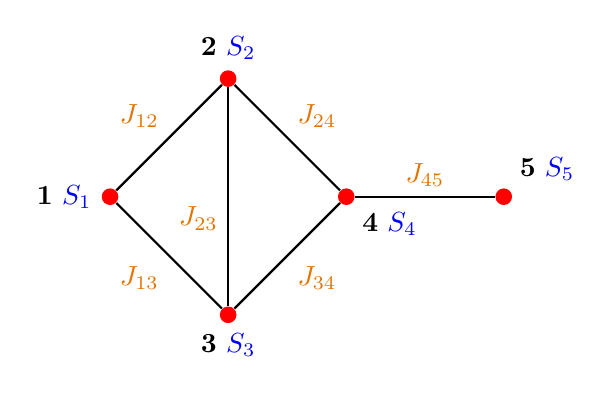
\begin{tikzpicture}[
        % Configuración de los nodos (puntos rojos)
        node/.style={circle, fill=red, inner sep=2pt, minimum size=6pt},
        % Configuración de las líneas (aristas)
        edge/.style={black, thick}
    ]
        
        % Definición de las posiciones de los vértices basándose en la cuadrícula
        \node[node, label=left:{\textbf{1} \color{blue}$S_1$}] (v1) at (0,0) {};
        \node[node, label=above:{\textbf{2} \color{blue}$S_2$}] (v2) at (1.5,1.5) {};
        \node[node, label=below:{\textbf{3} \color{blue}$S_3$}] (v3) at (1.5,-1.5) {};
        \node[node, label=below right:{\textbf{4} \color{blue}$S_4$}] (v4) at (3,0) {};
        \node[node, label=above right:{\textbf{5} \color{blue}$S_5$}] (v5) at (5,0) {};
        
        % Dibujado de aristas y colocación de etiquetas (J_ij) en color naranja/dorado
        \draw[edge] (v1) -- (v2) node[midway, above left, color=orange!90!black] {$J_{12}$};
        \draw[edge] (v1) -- (v3) node[midway, below left, color=orange!90!black] {$J_{13}$};
        \draw[edge] (v2) -- (v3) node[midway, below left, color=orange!90!black] {$J_{23}$};
        \draw[edge] (v2) -- (v4) node[midway, above right, color=orange!90!black] {$J_{24}$};
        \draw[edge] (v3) -- (v4) node[midway, below right, color=orange!90!black] {$J_{34}$};
        \draw[edge] (v4) -- (v5) node[midway, above, color=orange!90!black] {$J_{45}$};
        
    \end{tikzpicture}
    \caption{Grafo del Modelo de Ising correspondiente a la imagen.}
    \label{fig:ising_example}
\end{figure}

\subsubsection{Espacio de Estados y Variantes del Modelo}
\noindent 
Supongamos el caso particular donde todos los espines adoptan una orientación unánime hacia abajo, correspondiente al vector de estado $\underline{S} = (-1, -1, -1, -1, -1)$. La energía de este estado se reduce a la suma directa de sus acoplamientos. Por ejemplo, para el ejemplo antes visto tendríamos
\[
H(-1, -1, -1, -1, -1) = J_{12}(-1)(-1) + J_{13}(-1)(-1) + \dots = J_{12} + J_{13} + J_{23} + J_{24} + J_{34} + J_{45}
\]
Si imponemos una condición homogénea donde $J_{ij} = -J$ (siendo $J > 0$ un valor real fijo positivo) para todo par conectado, se desprenden las siguientes categorizaciones

\begin{enumerate}
    \item \textbf{Modelo de Ising Ferromagnético Tradicional:} Si los acoplamientos son constantes e idénticos ($J_{ij} = -J$), el signo negativo favorece energéticamente el alineamiento paralelo de los espines vecinos:
    \[
    H(\underline{S}) = -J \sum_{\langle i,j \rangle} S_i S_j
    \]
    \item \textbf{Vidrio de Espín de Ising (\textit{Spin Glass}):} Si las constantes de acoplamiento $J_{ij}$ dejan de ser fijas y se modelan como variables aleatorias independientes (ej. distribuciones Gaussianas), el sistema introduce desorden y frustración magnética.
\end{enumerate}

\subsubsection{Análisis Termodinámico y Unidades Energéticas}
\noindent 
La probabilidad de que el sistema exhiba una configuración geométrica concreta $\underline{S}$ en el equilibrio térmico viene dictada por la micro-medida canónica de Gibbs-Boltzmann:
\[
P(\underline{S}) \propto e^{-\beta H(\underline{S})}, \qquad \text{donde } \beta = \frac{1}{k_B T} \text{ (parámetro de temperatura inversa)}
\]
\begin{itemize}
    \item $k_B$: Constante de Boltzmann, cuyo valor experimental es $1.38 \cdot 10^{-23} \text{ Joules} \cdot \text{Kelvin}^{-1}$.
    \item $T$: Temperatura absoluta escalada en Kelvin ($T = t(^\circ\text{C}) + 273.15$).
\end{itemize}

\begin{ejemplo}
    Ejemplo de cálculo para Temperatura Ambiente ($T = 300\text{ K} \approx 27^\circ\text{C}$). La escala fundamental de energía térmica fluctuante ($\mathcal{E}$) se calcula como:
    \[
    \mathcal{E} = k_B T = (1.38 \cdot 10^{-23} \text{ J}\cdot\text{K}^{-1}) \cdot (300\text{ K}) = 4.14 \cdot 10^{-21} \text{ Joules}
    \]
    Haciendo uso de la equivalencia fundamental del electrón-voltio ($1 \text{ J} \approx 6.242 \cdot 10^{18} \text{ eV}$), transformamos la escala de energía:
    \[
    \mathcal{E} \approx 4.14 \cdot 10^{-21} \cdot (6.242 \cdot 10^{18}) \text{ eV} \approx 0.0258 \text{ eV} = 25.8 \text{ meV}
    \]

\end{ejemplo}



\begin{notacion}[Comportamiento Asintótico de la Temperatura]
La interacción entre la energía del Hamiltoniano y la agitación térmica del entorno viene gobernada de forma exclusiva por el producto adimensional $\beta J$. El comportamiento del sistema en los extremos térmicos dicta la física de las transiciones de fase:
\begin{itemize}
    \item \textbf{Límite de Baja Temperatura ($T \to 0^+$):} 
    \[
    T \to 0^+ \implies \beta = \frac{1}{k_B T} \to \infty \implies \beta J \to \infty
    \]
    En este régimen, el factor de Boltzmann $e^{-\beta H(\underline{S})}$ penaliza drásticamente cualquier estado excitado de energía alta. La medida de probabilidad colapsa casi con certeza ($c.s.$) sobre las configuraciones que minimizan el Hamiltoniano (estados fundamentales ordenados o ferromagnéticos, donde todos los espines apuntan en la misma dirección).
    
    \item \textbf{Límite de Alta Temperatura ($T \to \infty$):} 
    \[
    T \to \infty \implies \beta = \frac{1}{k_B T} \to 0 \implies \beta J \to 0
    \]
    Al anularse el argumento del exponente térmico, el factor de Boltzmann tiende a la unidad ($e^0 = 1$) para las $2^n$ configuraciones del espacio de estados $\mathcal{S}$. La medida de probabilidad se vuelve uniforme sobre todo el soporte discreto:
    \[
    P(\underline{S}) \to \frac{1}{2^n} \quad \forall \, \underline{S} \in \mathcal{S}
    \]
    El sistema alcanza el desorden absoluto (régimen paramagnético), donde la entropía satura el sistema y destruye cualquier correlación magnética entre primeros vecinos.
\end{itemize}
\end{notacion}

\subsubsection{Función de Partición y Deducción de la Energía Interna}

\noindent 
Para normalizar la medida de probabilidad de Gibbs sobre todo el espacio de configuraciones discretas, se define la \textbf{Función de Partición} (\textit{Zustandssumme}):
\[
Z(\beta) = \sum_{\underline{S}} e^{-\beta H(\underline{S})} \qquad \implies \qquad P(\underline{S}) = \frac{e^{-\beta H(\underline{S})}}{Z(\beta)}
\]
Efectuamos la derivada analítica de la función de partición respecto a la variable macroscópica $\beta$:
\[
\frac{dZ(\beta)}{d\beta} = \frac{d}{d\beta} \sum_{\underline{S}} e^{-\beta H(\underline{S})} = \sum_{\underline{S}} \frac{d}{d\beta} e^{-\beta H(\underline{S})} = \sum_{\underline{S}} -H(\underline{S}) e^{-\beta H(\underline{S})} = -\sum_{\underline{S}} H(\underline{S}) e^{-\beta H(\underline{S})}
\]
Por definición de la Mecánica Estadística, el valor esperado de la energía del sistema constituye la \textbf{Energía Interna Termodinámica ($U$)}:
\[
U = \langle H \rangle = \sum_{\underline{S}} H(\underline{S}) \cdot P(\underline{S}) = \frac{\sum_{\underline{S}} H(\underline{S}) e^{-\beta H(\underline{S})}}{Z(\beta)}
\]
Aislamos el término del sumatorio algebraico multiplicando por el signo opuesto, lo que nos permite conectar la esperanza con la derivada deducida previamente:
\[
U = -\frac{1}{Z(\beta)} \left( -\sum_{\underline{S}} H(\underline{S}) e^{-\beta H(\underline{S})} \right) = -\frac{1}{Z(\beta)} \frac{dZ(\beta)}{d\beta}
\]
Aplicando la regla de la cadena para la derivada de un logaritmo natural ($\frac{d}{dx} \ln(f(x)) = \frac{f'(x)}{f(x)}$), compactamos la expresión analítica final para la cantidad termodinámica fundamental $U$:
\[
\boxed{U = \langle H \rangle = -\frac{d \ln Z(\beta)}{d\beta}}
\]


\subsubsection{Potenciales Termodinámicos e Identidades Fundamentales}

\noindent
En el ensamble canónico (sistemas a volumen y temperatura constante en contacto con un baño térmico), el estado de equilibrio no se alcanza minimizando la energía interna $U$, sino minimizando el potencial de Helmholtz.

\begin{definicion}[Energía Libre de Helmholtz ($F$)]
    La \textbf{Energía Libre de Helmholtz} representa la fracción de energía interna del sistema que está disponible para realizar trabajo útil tras descontar el coste del desorden térmico. Se define analíticamente a partir de la función de partición mediante la identidad:
    \[
    F(\beta) = -\frac{1}{\beta} \ln Z(\beta) = -k_B T \ln Z
    \]
\end{definicion}

\begin{prop}[Transformada de Legendre y Entropía]
    La conexión macroscópica clásica entre la Energía Interna ($\mathcal{E} \equiv U = \langle H \rangle$), la temperatura y la Entropía ($S$) se formaliza a través de la relación fundamental:
    \[
    F = \mathcal{E} - TS
    \]
    Esta ecuación es la Transformada de Legendre que permite transicionar del colectivo microcanónico (donde domina el recuento de microestados $W$ vía $S = k_B \ln W$) al colectivo canónico regido por $Z(\beta)$. 
\end{prop}

\subsubsection{Operador de Magnetización ($M$) y Simetría del Sistema}
\noindent 
Para caracterizar cuantitativamente el orden magnético global de una configuración, introducimos la observable macroscópica \textbf{magnetización total} ($m(\underline{s})$).

\begin{definicion}
    La \tbf{magnetización total} de una configuración $\underline{s}$ se define como la suma algebraica de los espines individuales:
    \begin{equation*}
        m(\underline{s}) = \sum_{i=1}^{N} S_i
    \end{equation*}
\end{definicion}
Al calcular el valor esperado o primer momento estadístico de la magnetización ($E[M]$) promediado bajo la medida canónica de Gibbs, el sistema arroja una anulación simétrica absoluta debido a la isotropía espacial del Hamiltoniano:
\begin{equation*}
    E(M) = \sum_{\underline{s} \in \mathcal{S}} \frac{m(\underline{s}) e^{-\beta H(\underline{s}) Z}}{Z(\beta)} = 0
\end{equation*}
\observacion{
    A pesar de que el promedio simétrico es nulo ($E[M] = 0$), el valor esperado del módulo o magnitud absoluta de la magnetización es estrictamente positivo, \textbf{$\mathbb{E}[|M|] \neq 0$}. Esto denota que el cristal posee momentos magnéticos locales reales, pero carece de una dirección preferencial espontánea global en el ensamble canónico puro sin campo externo.
}


\begin{ejemplo}
Consideremos un sistema ferromagnético simple constituido por un grafo cerrado de tres vértices interconectados en forma de triángulo ($N=3$), visto en la Figura \ref{fig:ising_triangle}. El Hamiltoniano macroscópico del sistema, bajo constantes de acoplamiento homogéneas $J > 0$, responde a la sumatoria sobre primeros vecinos:
\[
H(\underline{S}) = -J(S_1S_2 + S_2S_3 + S_1S_3)
\]
El espacio de configuraciones posee un tamaño discreto de $2^3 = 8$ estados posibles. Al evaluar los espines, la energía se discretiza en dos únicos autoestados:
\begin{itemize}
    \item Energía $+J$: Asociada a $6$ configuraciones frustradas o no alineadas.
    \item Energía $-3J$: Asociada a $2$ estados perfectamente alineados.
\end{itemize}

\begin{figure}[htbp] % Es buena práctica añadir los especificadores de posición
    \centering % Reemplaza a \begin{center} ... \end{center}
    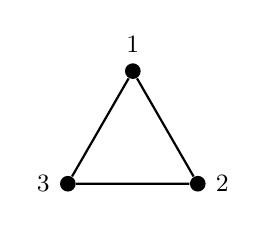
\begin{tikzpicture}[scale=1.1, baseline=(current bounding box.center)]
        % Nodos del grafo (V)
        \node[circle, fill=black, inner sep=2pt, label=above:{\small 1}] (v1) at (0.75,1.3) {};
        \node[circle, fill=black, inner sep=2pt, label=left:{\small 3}] (v3) at (0,0) {};
        \node[circle, fill=black, inner sep=2pt, label=right:{\small 2}] (v2) at (1.5,0) {};
        % Aristas o enlaces (E)
        \draw[thick] (v1) -- (v2) -- (v3) -- (v1);
    \end{tikzpicture}
    \caption{Grafo triangular para el Modelo de Ising.} % INDISPENSABLE para que el \label funcione correctamente
    \label{fig:ising_triangle} % Siempre debe ir DESPUÉS o DENTRO del \caption
\end{figure}
En la Tabla \ref{tab:ising_triangle} podemos ver la energía para todo el espacio de estados de $S$.

\begin{figure}
    \begin{center}
    \small
    \begin{tabular}{ccc|lc|c}
    $S_1$ & $S_2$ & $S_3$ & Producto de Pares Varianza & Suma del Paréntesis & Energía $H(\underline{S})$ \\
    \hline
    $-1$ & $-1$ & $-1$ & $(+1) + (+1) + (+1)$ & $+3$ & $-3J$ \\
    $+1$ & $-1$ & $-1$ & $(-1) + (+1) + (-1)$ & $-1$ & $+J$ \\
    $-1$ & $+1$ & $-1$ & $(-1) + (-1) + (+1)$ & $-1$ & $+J$ \\
    $-1$ & $-1$ & $+1$ & $(+1) + (-1) + (-1)$ & $-1$ & $+J$ \\
    $+1$ & $+1$ & $-1$ & $(+1) + (-1) + (-1)$ & $-1$ & $+J$ \\
    $+1$ & $-1$ & $+1$ & $(-1) + (-1) + (+1)$ & $-1$ & $+J$ \\
    $-1$ & $+1$ & $+1$ & $(-1) + (+1) + (-1)$ & $-1$ & $+J$ \\
    $+1$ & $+1$ & $+1$ & $(+1) + (+1) + (+1)$ & $+3$ & $-3J$ \\
    \end{tabular}
    \end{center}
    \caption{Tabla de Energías para el Modelo de Ising Triangular.}
    \label{tab:ising_triangle}
\end{figure}
\noindent 
Tomando como base las degeneraciones obtenidas en el recuento microcanónico de la tabla (2 estados estables y 6 degenerados), la \textbf{Función de Partición} $Z(\beta)$ se condensa analíticamente como:
\[
Z(\beta) = \sum_{\underline{s} \in \mathcal{S}} e^{-\beta H(\underline{s})} = 2e^{-\beta(-3J)} + 6e^{-\beta(+J)} = 2e^{3\beta J} + 6e^{-\beta J}
\]
A partir de la función de partición canónica, derivamos la \textbf{Energía Libre de Helmholtz ($F$)} del cristal:
\[
F = -\frac{1}{\beta} \log Z(\beta) = -\frac{1}{\beta} \log\left(2e^{3\beta J} + 6e^{-\beta J}\right)
\]
Calculamos el valor esperado de la energía o \textbf{Energía Interna Termodinámica ($E \equiv \langle H \rangle$)} ejecutando el operador diferencial canónico $-\frac{1}{Z}\frac{dZ}{d\beta}$:
\[
E = -\frac{1}{Z(\beta)} \frac{dZ(\beta)}{d\beta} = -\frac{1}{Z(\beta)} \left(2 \cdot 3J \cdot e^{3\beta J} + 6 \cdot (-J) \cdot e^{-\beta J}\right) = -\frac{6J e^{3\beta J} - 6J e^{-\beta J}}{2e^{3\beta J} + 6e^{-\beta J}}
\]
Factorizando y simplificando el signo negativo del numerador, el promedio de energía se compacta como:
\[
E = 6J \, \frac{e^{-\beta J} - e^{3\beta J}}{6e^{-\beta J} + 2e^{3\beta J}}
\]

\noindent 
Evaluemos el comportamiento asintótico de la energía interna bajo los dos extremos de la escala térmica:
\[
\lim_{\beta J \to 0} E = 6J \, \frac{1 - 1}{6 + 2} = 0 \qquad \left[\text{Límite de Alta Temperatura } T \to \infty\right]
\]
\[
\lim_{\beta J \to +\infty} E = \lim_{\beta J \to +\infty} 6J \, \frac{\cancel{e^{-\beta J}} - e^{3\beta J}}{\cancel{6e^{-\beta J}} + 2e^{3\beta J}} = 6J \left( \frac{-e^{3\beta J}}{2e^{3\beta J}} \right) = -3J \qquad \left[\text{Límite de Cero Absoluto } T \to 0^+\right]
\]
Haciendo uso de la ecuación puente de la entropía deducida por la transformada de Legendre ($\frac{S}{k_B} = \beta(E - F)$), extendemos la función funcional completa del desorden:
\[
\frac{S}{k_B} = \beta \left[ 6J \, \frac{e^{-\beta J} - e^{3\beta J}}{6e^{-\beta J} + 2e^{3\beta J}} + \frac{1}{\beta} \log\left(2e^{3\beta J} + 6e^{-\beta J}\right) \right] = 6\beta J \, \frac{e^{-\beta J} - e^{3\beta J}}{6e^{-\beta J} + 2e^{3\beta J}} + \log\left(2e^{3\beta J} + 6e^{-\beta J}\right)
\]
\textit{Nota Analítica:} Al evaluar de forma directa el límite de baja temperatura ($\beta J \to \infty$), la estructura colapsa en una indeterminación de tipo $[-\infty + \infty]$. Procedemos a su resolución aplicando el comportamiento asintótico de los términos exponenciales dominantes:

\begin{enumerate}
    \item \textbf{Aproximación del término logarítmico ($F$):}
    \[
    \log\left(2e^{3\beta J} + 6\cancelto{0}{e^{-\beta J}}\right) \approx \log\left(2e^{3\beta J}\right) = \log(2) + \log\left(e^{3\beta J}\right) = \log(2) + 3\beta J
    \]
    \item \textbf{Aproximación del término fraccionario ($E$):}
    \[
    6\beta J \, \frac{\cancelto{0}{e^{-\beta J}} - e^{3\beta J}}{\cancelto{0}{6e^{-\beta J}} + 2e^{3\beta J}} \approx 6\beta J \left( \frac{-e^{3\beta J}}{2e^{3\beta J}} \right) = -3\beta J
    \]
\end{enumerate}
Sustituyendo ambas simplificaciones asintóticas en la ecuación de la entropía, los infinitos lineales de la temperatura inversa se cancelan de forma exacta, resolviendo la indeterminación:
\[
\lim_{\beta J \to \infty} \frac{S}{k_B} = -3\beta J + \log(2) + 3\beta J = \boxed{\log(2)}
\]
El resumen de los límites de la entropía queda como
\begin{align*}
    \lim_{\beta J \to 0} \frac{S}{k_B} &= \log(8) \quad \text{\small (Saturación de desorden: Equiprobabilidad en los 8 microestados)} \\
    \lim_{\beta J \to \infty} \frac{S}{k_B} &= \log(2) \quad \text{\small (Orden latente: El sistema se congela en los 2 estados fundamentales)}
\end{align*}
\end{ejemplo}

\section{Reversible Markov Chain}
Recordemos la definición de cadena de Márkov reversible.
\begin{definicion}[Balance Detallado]
    Se dice que una cadena de Markov discreta con matriz de transición $P = (p_{ij})$ es \textbf{reversible} respecto a una distribución de probabilidad macroscópica $\pi = (\pi_i)_{i \in \mathcal{S}}$ si satisface de manera unívoca el sistema de ecuaciones algebraicas lineales denominado \textbf{Condición de Balance Detallado}:
    \[
    p_{ij} \pi_j = p_{ji} \pi_i \quad \forall \, (i,j) \in \mathcal{S} \times \mathcal{S}
    \]
    Físicamente, esta condición impone una simetría estadística temporal absoluta: el flujo neto de probabilidad que transita desde el estado $j$ hacia el estado $i$ en equilibrio es idéntico al flujo en sentido inverso. Una consecuencia analítica directa de este principio es que cualquier distribución $\pi$ que verifique el balance detallado constituye automáticamente una \textbf{distribución estacionaria e invariante} del proceso ($\pi = \pi P$).
\end{definicion}

\subsection{Acoplamiento de la Dinámica de Markov al Modelo de Ising}

\noindent Para resolver el Modelo de Ising mediante simulación, definimos una cadena de Markov donde cada estado en un instante temporal $t$ es una configuración microscópica completa de espines espaciales $\mathcal{S}(t) = \underline{s}$. La probabilidad de transición condicional para transicionar hacia un estado de prueba consecutivo $\underline{s}'$ se denota como:
\[
P(\mathcal{S}(t+1) = \underline{s}' \mid \mathcal{S}(t) = \underline{s}) = P(\underline{s}' \mid \underline{s}) = p_{\underline{s} \, \underline{s}'}
\]
Exigimos que este proceso estocástico artificial satisfaga el balance detallado con respecto a la medida canónica invariante de Gibbs-Boltzmann, denotada aquí como $\mu(\underline{s})$:
\[
P(\underline{s}' \mid \underline{s}) \mu(\underline{s}) = P(\underline{s} \mid \underline{s}') \mu(\underline{s}') \quad \forall \, (\underline{s}, \underline{s}') \in \mathcal{S} \times \mathcal{S}
\]
Sustituyendo explícitamente la estructura analítica de la distribución de Gibbs de tus apuntes en ambos miembros de la ecuación, cancelamos algebraicamente el factor de normalización común correspondiente a la función de partición $Z(\beta)$:
\[
P(\underline{s}' \mid \underline{s}) \, \frac{e^{-\beta H(\underline{s})}}{\cancel{Z(\beta)}} = P(\underline{s} \mid \underline{s}') \, \frac{e^{-\beta H(\underline{s}')}}{\cancel{Z(\beta)}}
\]
Agrupando los términos de transiciones probabilísticas en el miembro izquierdo y las funciones exponenciales de energía en el derecho, aislamos el cociente de probabilidades de transición:
\[
\frac{P(\underline{s}' \mid \underline{s})}{P(\underline{s} \mid \underline{s}')} = \frac{e^{-\beta H(\underline{s}')}}{e^{-\beta H(\underline{s})}} = e^{-\beta (H(\underline{s}') - H(\underline{s}))} = e^{-\beta \Delta H}
\]
Donde $\Delta H = H(\underline{s}') - H(\underline{s})$ define el balance diferencial de energía macroscópica asociado al salto microscópico cristalino.

\subsection{Metropolis Algorithm}

\noindent 
Para garantizar de manera unívoca el cumplimiento de la relación cinemática 
$$\frac{P(\underline{s}' \mid \underline{s})}{P(\underline{s} \mid \underline{s}')} = e^{-\beta \Delta H}$$ 
sobre un computador, Metropolis y su equipo dividieron la probabilidad de transición en dos fases consecutivas independientes: la probabilidad de proponer un estado $q(\underline{s}' \mid \underline{s})$ (simétrica) y la probabilidad de aceptarlo $\alpha(\underline{s}' \mid \underline{s})$. Esto formaliza el siguiente procedimiento iterativo de muestreo estocástico:


\begin{teo}[Metropolis Algorithm]
Dada una configuración de partida y una temperatura inversa fija $\beta$, el proceso evoluciona de acuerdo con las siguientes reglas estocásticas paso a paso:
\begin{enumerate}
    \item[\textbf{\color{red}1)}] \textbf{Inicialización:} Comenzar la simulación desde un estado de espín macroscópico inicial $\underline{s}$.
    
    \item[\textbf{\color{red}2)}] \textbf{Mutación Local:} Seleccionar un único espín de la red cristalina de forma aleatoria uniforme e invertir su orientación ($S_i \to -S_i$) para construir una configuración de prueba tentativa denotada como $\underline{s}'$.
    
    \item[\textbf{\color{red}3)}] \textbf{Evaluación Energética:} Computar la barrera de energía potencial entre ambos estados calculando el gradiente local del Hamiltoniano:
    \[
    \Delta H = H(\underline{s}') - H(\underline{s})
    \]
    
    \item[\textbf{\color{red}4)}] \textbf{Criterio de Descenso Energético:} Si $\Delta H \le 0$, el movimiento propuesto conduce a una configuración energéticamente más estable o degenerada. El sistema \textbf{acepta el movimiento con probabilidad unitaria}: se almacena $\underline{s}'$ como el nuevo estado actual de la cadena y se reinicia el ciclo desde el Paso 2.
    
    \item[\textbf{\color{red}5)}] \textbf{Criterio de Activación Térmica ($\Delta H > 0$):} Si el movimiento propuesto impone un sobrecoste energético, la transición se ve condicionada por las fluctuaciones del baño térmico. Se selecciona un número pseudoaleatorio auxiliar $\alpha$ muestreado bajo una distribución uniforme continua en el intervalo abierto estándar:
    \[
    \alpha \sim U(0,1)
    \]
    
    \item[\textbf{\color{red}6)}] \textbf{Aceptación Estocástica:} Si el umbral aleatorio satisface la desigualdad:
    \[
    \alpha < e^{-\beta \Delta H}
    \]
    Se acepta la transición a pesar del incremento energético. Se guarda $\underline{s}'$ como el siguiente eslabón de la trayectoria y se reinicia el ciclo.
    
    \item[\textbf{\color{red}7)}] \textbf{Rechazo y Conservación de Masa:} Si no se cumple la desigualdad anterior, el movimiento de prueba es denegado. El sistema permanece estático haciendo $\underline{s} = \underline{s}$. Se vuelve a registrar la configuración original $\underline{s}$ como el estado consecutivo de la serie cronológica (acumulando peso estadístico en el histograma de ocupación) y se reinicia el proceso.
\end{enumerate}
\end{teo}

